\documentclass[12pt,a4paper]{report}

% ==============================================================================
% PACKAGES AND SETUP FOR SR UNIVERSITY ACADEMIC REPORT
% ==============================================================================
\usepackage[a4paper, top=1in, bottom=1in, left=1.25in, right=1in]{geometry}
\usepackage{mathptmx} % Times New Roman font for standard academic reports
\usepackage{setspace}
\onehalfspacing

\usepackage{graphicx}
\usepackage{amsmath, amssymb}
\usepackage{booktabs, tabularx, longtable, multirow, array}
\usepackage{caption, subcaption}
\usepackage{float}
\usepackage{enumitem}
\usepackage{microtype}
\usepackage{xcolor}
\usepackage{listings}
\usepackage{fancyhdr}
\usepackage{titlesec}
\usepackage{cite}

% TikZ Configuration for Architecture, Flowcharts, and UML Diagrams
\usepackage{tikz}
\usetikzlibrary{
    shapes.geometric,
    shapes.multipart,
    arrows.meta,
    positioning,
    calc,
    fit,
    backgrounds,
    matrix,
    shadows
}

% Hyperref configuration for clickable PDF links and bookmarks
\usepackage[
    colorlinks=true,
    linkcolor=black,
    citecolor=blue!70!black,
    urlcolor=blue!70!black,
    pdfauthor={J.kowshik},
    pdftitle={Customer Relationship Management (CRM) System - SR University Project Report},
    pdfsubject={DevOps and Full Stack Development Capstone Report},
    pdfkeywords={CRM, MERN, React, Node, Express, MongoDB, DevOps, Docker, Kubernetes, Vercel, Render}
]{hyperref}

% Define Custom Colors for Listings and Diagram Elements
\definecolor{codegreen}{rgb}{0,0.6,0}
\definecolor{codegray}{rgb}{0.5,0.5,0.5}
\definecolor{codepurple}{rgb}{0.58,0,0.82}
\definecolor{backcolour}{rgb}{0.97,0.98,0.99}
\definecolor{navy}{RGB}{15, 34, 64}
\definecolor{slate}{RGB}{70, 80, 95}

% Code Listing Configuration
\lstdefinestyle{mystyle}{
    backgroundcolor=\color{backcolour},   
    commentstyle=\color{codegreen},
    keywordstyle=\color{blue!80!black}\bfseries,
    numberstyle=\tiny\color{codegray},
    stringstyle=\color{codepurple},
    basicstyle=\ttfamily\footnotesize,
    breakatwhitespace=false,         
    breaklines=true,                 
    captionpos=b,                    
    keepspaces=true,                 
    numbers=left,                    
    numbersep=6pt,                  
    showspaces=false,                
    showstringspaces=false,
    showtabs=false,                  
    tabsize=2,
    frame=single,
    rulecolor=\color{gray!30}
}
\lstset{style=mystyle}

% Header and Footer Styling
\pagestyle{fancy}
\fancyhf{}
\fancyhead[L]{\fontsize{9}{11}\selectfont \nouppercase{\leftmark}}
\fancyhead[R]{\fontsize{9}{11}\selectfont SR UNIVERSITY}
\fancyfoot[C]{\thepage}
\renewcommand{\headrulewidth}{0.5pt}
\renewcommand{\footrulewidth}{0.5pt}

% Adjust plain page style for chapter beginnings
\fancypagestyle{plain}{
    \fancyhf{}
    \fancyfoot[C]{\thepage}
    \renewcommand{\headrulewidth}{0pt}
    \renewcommand{\footrulewidth}{0.5pt}
}

% Chapter and Section Heading Typography
\titleformat{\chapter}[display]
  {\normalfont\fontsize{18}{22}\bfseries\color{navy}}
  {\filleft\fontsize{14}{18}\selectfont\textbf{CHAPTER \thechapter}}
  {1ex}
  {\titlerule[1pt]\vspace{1ex}\filright}
  [\vspace{1ex}\titlerule]

\titleformat{\section}
  {\normalfont\fontsize{14}{17}\bfseries\color{navy}}
  {\thesection}{1em}{}

\titleformat{\subsection}
  {\normalfont\fontsize{12}{15}\bfseries\color{slate}}
  {\thesubsection}{1em}{}

% ==============================================================================
% DOCUMENT BODY
% ==============================================================================
\begin{document}

% ------------------------------------------------------------------------------
% PRELIMINARY PAGES (ROMAN NUMBERING)
% ------------------------------------------------------------------------------
\pagenumbering{roman}

% Preliminary Pages for SR University Project Report

% ==============================================================================
% 1. COVER / TITLE PAGE
% ==============================================================================
\begin{titlepage}
\begin{center}
    \vspace*{-1cm}
    
\includegraphics[width=4.5cm]{figures/sru_logo.png}\\[0.6cm]
    
    {\fontsize{18}{22}\selectfont \textbf{SR UNIVERSITY}}\\[0.2cm]
    {\fontsize{13}{16}\selectfont \textbf{SCHOOL OF COMPUTER SCIENCE \& ARTIFICIAL INTELLIGENCE}}\\[0.6cm]
    
    {\fontsize{14}{17}\selectfont \textbf{COURSE PROJECT REPORT}}\\[0.4cm]
    
    \rule{\linewidth}{1.2pt}\\[0.4cm]
    {\fontsize{20}{24}\selectfont \textbf{CUSTOMER RELATIONSHIP MANAGEMENT}}\\[0.2cm]
    {\fontsize{20}{24}\selectfont \textbf{(CRM) SYSTEM}}\\[0.2cm]
    {\fontsize{12}{15}\selectfont \textit{A Cloud-Native MERN Stack Enterprise Application with Role-Based Access Control, Real-Time Analytics, and DevOps Automation}}\\[0.3cm]
    \rule{\linewidth}{1.2pt}\\[0.5cm]
    
    {\fontsize{12}{15}\selectfont Submitted in partial fulfilment of the requirements for the course}\\[0.2cm]
    {\fontsize{14}{17}\selectfont \textbf{DEVOPS AND FULL STACK DEVELOPMENT}}\\[0.5cm]
    
    \begin{table}[h!]
    \centering
    \renewcommand{\arraystretch}{1.3}
    \begin{tabular}{|p{4.5cm}|p{9.5cm}|}
    \hline
    \textbf{Student Details} & \textbf{Information} \\ \hline
    \textbf{Student HT No.} & 2303A51759 \\ \hline
    \textbf{Student Name} & J.kowshik \\ \hline
    \textbf{Faculty Coordinator} & Dr. Mohammed Ali Shaik, Professor \\ \hline
    \textbf{Designation} & Professor, School of Computer Science \& AI \\ \hline
    \textbf{School} & School of Computer Science \& Artificial Intelligence \\ \hline
    \textbf{Academic Year} & 2026--2027 \\ \hline
    \textbf{Semester} & I (B.Tech IV Year) \\ \hline
    \textbf{Course Code} & 23CS102PE405 \\ \hline
    \textbf{GitHub Repository} & \url{https://github.com/Kowshik1759/CRM-System} \\ \hline
    \textbf{Frontend Deployment} & \url{https://crm-system-sable-delta.vercel.app} \\ \hline
    \textbf{Backend Deployment} & \url{https://crm-system-ea6d.onrender.com} \\ \hline
    \textbf{Database Infrastructure} & MongoDB Atlas Cloud (\texttt{crm\_db}) \\ \hline
    \end{tabular}
    \end{table}
    
    \vfill
    {\fontsize{11}{14}\selectfont 
    \textbf{SR UNIVERSITY}\\
    Ananthasagar, Hasanparthy, Warangal, Telangana, India -- 506371\\
    \url{www.sru.edu.in}}\\[0.3cm]
    {\fontsize{10}{13}\selectfont November 2026}
\end{center}
\end{titlepage}

% ==============================================================================
% 2. CERTIFICATE
% ==============================================================================
\newpage
\thispagestyle{plain}
\begin{center}
    
\includegraphics[width=3cm]{figures/sru_logo.png}\\[0.3cm]
    {\fontsize{16}{20}\selectfont \textbf{SR UNIVERSITY}}\\[0.1cm]
    {\fontsize{12}{15}\selectfont \textbf{SCHOOL OF COMPUTER SCIENCE \& ARTIFICIAL INTELLIGENCE}}\\[0.1cm]
    {\fontsize{11}{14}\selectfont Ananthasagar, Hasanparthy, Warangal, Telangana, India -- 506371}\\[0.5cm]
    
    {\fontsize{16}{20}\selectfont \textbf{CERTIFICATE OF ORIGINAL WORK}}\\[0.6cm]
\end{center}

\noindent This is to certify that the project report entitled \textbf{``CUSTOMER RELATIONSHIP MANAGEMENT (CRM) SYSTEM''} submitted by \textbf{J.kowshik} (Hall Ticket No: \textbf{2303A51759}) in partial fulfilment of the requirements for the award of the degree in the course \textbf{DevOps and Full Stack Development (Course Code: 23CS102PE405)} during the academic year \textbf{2026--2027}, is a bonafide record of the work carried out under my supervision and guidance.

\vspace{0.4cm}
\noindent The technical implementation, cloud deployments on Vercel, Render, and MongoDB Atlas, automated tests, and documentation presented in this report have been verified and evaluated for technical accuracy and academic excellence.

\vspace{2.5cm}
\noindent
\begin{tabular*}{\textwidth}{@{\extracolsep{\fill}}ccc}
    \rule{4.5cm}{0.8pt} & \rule{4.5cm}{0.8pt} & \rule{4.5cm}{0.8pt} \\
    \textbf{Faculty Guide} & \textbf{Head of the Department} & \textbf{External Examiner} \\
    Dr. Mohammed Ali Shaik & Dr. [HOD NAME] & [EXTERNAL EXAMINER] \\
    Professor, SCSAI & Professor \& Head, SCSAI & Department of CSE \\
    SR University & SR University & External Evaluation
\end{tabular*}

% ==============================================================================
% 3. DECLARATION
% ==============================================================================
\newpage
\thispagestyle{plain}
\begin{center}
    {\fontsize{16}{20}\selectfont \textbf{DECLARATION}}\\[0.6cm]
\end{center}

\noindent I, \textbf{J.kowshik}, student of B.Tech Computer Science and Artificial Intelligence, School of Computer Science \& Artificial Intelligence, SR University, bearing Hall Ticket Number \textbf{2303A51759}, hereby declare that the project entitled \textbf{``CUSTOMER RELATIONSHIP MANAGEMENT (CRM) SYSTEM''} is an original piece of work designed and developed by me under the supervision of \textbf{Dr. Mohammed Ali Shaik}, Professor, School of Computer Science \& Artificial Intelligence.

\vspace{0.4cm}
\noindent I further declare that this report has been compiled in partial fulfilment of the academic requirements for the course \textbf{DevOps and Full Stack Development (23CS102PE405)} during the academic year \textbf{2026--2027}. The software system, including its source code, architectural configurations, REST API endpoints, user interfaces, and automated deployments, has been constructed in accordance with professional software engineering principles.

\vspace{0.4cm}
\noindent To the best of my knowledge, this report has not been submitted previously in part or in full to any other university or academic institution for the award of any diploma or degree.

\vspace{2.5cm}
\noindent
\begin{tabular*}{\textwidth}{@{\extracolsep{\fill}}lr}
    \textbf{Date:} 15th November 2026 & \rule{5cm}{0.8pt} \\
    \textbf{Place:} Warangal, Telangana & \textbf{J.kowshik} \\
    & \textbf{HT No:} 2303A51759
\end{tabular*}

% ==============================================================================
% 4. ACKNOWLEDGEMENT
% ==============================================================================
\newpage
\thispagestyle{plain}
\begin{center}
    {\fontsize{16}{20}\selectfont \textbf{ACKNOWLEDGEMENT}}\\[0.6cm]
\end{center}

\noindent I express my profound gratitude and heartfelt thanks to \textbf{Dr. Mohammed Ali Shaik}, Professor, School of Computer Science \& Artificial Intelligence, SR University, for his invaluable guidance, technical scrutiny, and encouragement throughout the ideation, implementation, and deployment phases of this project.

\vspace{0.4cm}
\noindent I would like to extend my sincere thanks to the \textbf{Dean} and the \textbf{Head of the School of Computer Science \& Artificial Intelligence}, SR University, for providing the necessary academic infrastructure, cloud development computing labs, and environment required to undertake this capstone project.

\vspace{0.4cm}
\noindent My sincere appreciation also goes to all the faculty members of the School of Computer Science \& Artificial Intelligence for imparting strong foundational knowledge in web technologies, distributed database architectures, software testing, and DevOps methodologies.

\vspace{0.4cm}
\noindent Finally, I wish to express my deepest gratitude to my parents, family members, and peers for their continuous moral support, understanding, and motivation throughout the course of this academic endeavour.

\vspace{2cm}
\noindent
\begin{flushright}
    \textbf{J.kowshik}\\
    Hall Ticket No: \textbf{2303A51759}\\
    Department of Computer Science \& Artificial Intelligence\\
    SR University, Warangal
\end{flushright}

% ==============================================================================
% 5. ABSTRACT
% ==============================================================================
\newpage
\thispagestyle{plain}
\begin{center}
    {\fontsize{16}{20}\selectfont \textbf{ABSTRACT}}\\[0.6cm]
\end{center}

\noindent Modern small-to-medium enterprises (SMEs) face critical operational inefficiencies due to fragmented customer data, manual lead tracking via spreadsheets, disconnected task delegation, and the absence of consolidated sales analytics. Conventional enterprise customer relationship management (CRM) platforms often impose cost-prohibitive licensing, complex onboarding workflows, and rigid monolithic architectures that are ill-suited for agile business environments. 

This project presents the design, development, verification, and cloud-native deployment of a comprehensive, production-grade \textbf{Customer Relationship Management (CRM) System} engineered on the MERN technology stack (MongoDB, Express.js, React.js, Node.js) paired with modern DevOps infrastructure. The system is architected as a decoupled three-tier enterprise web application featuring:
\begin{enumerate}[label=(\roman*)]
    \item A high-performance, single-page application (SPA) frontend developed using React 18, Vite, Tailwind CSS, Lucide icons, and Recharts, delivering twelve fully interactive, responsive operational screens;
    \item A secure, stateless backend REST API engineered with Node.js and Express.js, implementing JSON Web Token (JWT) authentication, bcrypt password hashing, centralized error handling, and hierarchical Role-Based Access Control (RBAC) across four distinct enterprise personas: \textit{Admin}, \textit{Sales Manager}, \textit{Sales Executive}, and \textit{Customer Support};
    \item A scalable cloud data tier powered by MongoDB Atlas utilizing the Mongoose Object-Document Mapper (ODM), featuring automated data bootstrapping, compound indexes, relational document population, and complex multi-stage aggregation pipelines for real-time reporting;
    \item An interactive Kanban-style visual sales pipeline enabling drag-and-drop opportunity stage progression across six standardized qualification stages;
    \item Four mandatory regulatory analytical reports (Lead Conversion Funnel, Sales Team Performance, Customer Demographics Details, and Follow-Up Activity Matrix) dynamically rendered from live database aggregations with CSV export capabilities;
    \item A modern DevOps lifecycle incorporating Git version control, multi-stage Docker containerization with Nginx reverse proxying, Kubernetes deployment manifests with liveness and readiness health probes, automated static routing via Vercel, and continuous backend hosting on Render.
\end{enumerate}

The complete system has been subjected to rigorous end-to-end testing, verifying all CRUD operations, RBAC boundary enforcement, API response latencies, and persistent multi-tenant workflows. The production application is publicly hosted on Vercel (\url{https://crm-system-sable-delta.vercel.app}) and Render (\url{https://crm-system-ea6d.onrender.com}), demonstrating academic rigor and enterprise-ready software craftsmanship.

\vspace{0.6cm}
\noindent \textbf{Keywords:} Customer Relationship Management (CRM), MERN Stack, React 18, Vite, Node.js, Express.js, MongoDB Atlas, Role-Based Access Control (RBAC), DevOps, Docker, Kubernetes, Vercel, Render.

% ==============================================================================
% 6. LIST OF ABBREVIATIONS
% ==============================================================================
\newpage
\thispagestyle{plain}
\begin{center}
    {\fontsize{16}{20}\selectfont \textbf{LIST OF ABBREVIATIONS}}\\[0.6cm]
\end{center}

\begin{table}[h!]
\centering
\renewcommand{\arraystretch}{1.25}
\begin{tabular}{|p{3cm}|p{11.5cm}|}
\hline
\textbf{Abbreviation} & \textbf{Full Expansion} \\ \hline
\textbf{API} & Application Programming Interface \\ \hline
\textbf{Bcrypt} & Blowfish-based Password Hashing Algorithm \\ \hline
\textbf{CI/CD} & Continuous Integration / Continuous Deployment \\ \hline
\textbf{CORS} & Cross-Origin Resource Sharing \\ \hline
\textbf{CRUD} & Create, Read, Update, Delete \\ \hline
\textbf{CRM} & Customer Relationship Management \\ \hline
\textbf{CSS} & Cascading Style Sheets \\ \hline
\textbf{DFD} & Data Flow Diagram \\ \hline
\textbf{DNS} & Domain Name System \\ \hline
\textbf{DOM} & Document Object Model \\ \hline
\textbf{E2E} & End-to-End Testing \\ \hline
\textbf{ERD} & Entity-Relationship Diagram \\ \hline
\textbf{HTML} & HyperText Markup Language \\ \hline
\textbf{HTTP / HTTPS} & HyperText Transfer Protocol / Secure \\ \hline
\textbf{IEEE} & Institute of Electrical and Electronics Engineers \\ \hline
\textbf{JSON} & JavaScript Object Notation \\ \hline
\textbf{JWT} & JSON Web Token \\ \hline
\textbf{K8s} & Kubernetes Orchestration System \\ \hline
\textbf{KPI} & Key Performance Indicator \\ \hline
\textbf{MERN} & MongoDB, Express.js, React.js, Node.js \\ \hline
\textbf{NFR} & Non-Functional Requirement \\ \hline
\textbf{NoSQL} & Not Only Structured Query Language (Document Database) \\ \hline
\textbf{ODM} & Object-Document Mapper \\ \hline
\textbf{OS} & Operating System \\ \hline
\textbf{RBAC} & Role-Based Access Control \\ \hline
\textbf{REST} & Representational State Transfer \\ \hline
\textbf{SME} & Small and Medium-sized Enterprises \\ \hline
\textbf{SPA} & Single Page Application \\ \hline
\textbf{SQL} & Structured Query Language \\ \hline
\textbf{SRU} & SR University \\ \hline
\textbf{TLS / SSL} & Transport Layer Security / Secure Sockets Layer \\ \hline
\textbf{UI / UX} & User Interface / User Experience \\ \hline
\textbf{UML} & Unified Modeling Language \\ \hline
\textbf{URI / URL} & Uniform Resource Identifier / Uniform Resource Locator \\ \hline
\textbf{VCS} & Version Control System \\ \hline
\textbf{YAML} & YAML Ain't Markup Language \\ \hline
\end{tabular}
\end{table}


\newpage
\tableofcontents

\newpage
\listoffigures

\newpage
\listoftables

% ------------------------------------------------------------------------------
% MAIN CHAPTERS (ARABIC NUMBERING)
% ------------------------------------------------------------------------------
\newpage
\pagenumbering{arabic}
\setcounter{page}{1}

% Chapter 1: Introduction
\chapter{INTRODUCTION}

\section{Introduction}
Customer Relationship Management (CRM) has evolved from a basic contact management database into an essential operational pillar for modern commercial enterprises. In an increasingly competitive global economy, small and medium-sized enterprises (SMEs) require agile, reliable, and scalable software solutions to coordinate customer acquisition, sales pipeline progression, support interactions, and operational reporting. 

This project entails the comprehensive design, architectural development, and cloud-native deployment of an enterprise-grade \textbf{Customer Relationship Management (CRM) System for Small Businesses} built on the MERN technology stack (MongoDB, Express.js, React.js, and Node.js). Engineered to bridge the gap between rudimentary academic prototypes and commercial software offerings, the system delivers twelve specialized operational screens, four hierarchical Role-Based Access Control (RBAC) personas, automated visual sales pipelines, and dynamic MongoDB aggregation-backed analytics.

\section{Background of Customer Relationship Management}
Historically, business interactions and customer records were preserved through physical paper ledgers, rolodexes, and subsequently disconnected desktop spreadsheets. As demonstrated by Payne and Frow~\cite{payne2005strategic}, a successful CRM implementation represents a strategic cross-functional integration of processes, people, operations, and technological capabilities aimed at delivering superior customer value and operational transparency.

In early digital workflows, companies relied on fragmented productivity suites where customer contacts resided in one spreadsheet, sales leads in another, and pending customer support complaints in manual email threads. Reinartz et al.~\cite{reinartz2004customer} identified that failure to systematically track the customer lifecycle—from initial lead capture through proposal negotiation, closing, and post-sale retention—results in substantial revenue leakage, customer churn, and operational friction. Consequently, centralized web-based CRM architectures have emerged as an industry necessity, facilitating unified visibility and collaboration across distributed sales and support teams.

\section{Problem Statement}
Small and growing commercial businesses frequently operate with constrained IT budgets, limited technical staff, and highly dynamic sales workflows. Commercial enterprise CRM platforms (e.g., Salesforce, HubSpot, SAP) present severe operational obstacles for SMEs:
\begin{enumerate}[label=(\alph*)]
    \item \textbf{Prohibitive Cost Structures:} Subscription fees scaling per-user per-month render enterprise suites economically unviable for lean startups and regional businesses.
    \item \textbf{Architectural Bloat and Complexity:} Heavy enterprise suites include hundreds of unnecessary enterprise features, requiring extensive configuration, weeks of employee onboarding, and dedicated system administrators.
    \item \textbf{Data Silos and Redundancy:} Informal tools such as Excel and Google Sheets lack relational referential integrity, automated concurrency control, role-based security boundaries, and auditability.
    \item \textbf{Absence of Real-Time Analytics:} Without automated data aggregation, managers cannot readily ascertain the real-time health of the sales pipeline, team conversion percentages, or pending follow-up bottlenecks.
\end{enumerate}
There exists an acute need for a lightweight, modular, cloud-native, and secure CRM system tailored specifically for small business dynamics, providing enterprise-quality usability, zero licensing costs, and robust DevOps delivery.

\section{Objectives of the Project}
The primary objective of this project is to build and deploy a production-grade, full-stack Customer Relationship Management web application that fulfills the following goals:
\begin{enumerate}[label=\textbf{OBJ-\arabic*}:]
    \item \textbf{Decoupled Modern Architecture:} Architect a decoupled three-tier web application using React 18, Vite, Node.js, Express.js, and MongoDB Atlas.
    \item \textbf{Hierarchical Access Control:} Implement strict Role-Based Access Control (RBAC) supporting four distinct organizational tiers: \textit{Admin}, \textit{Sales Manager}, \textit{Sales Executive}, and \textit{Customer Support}, enforcing permissions on both frontend route guards and backend API middleware.
    \item \textbf{Comprehensive Module Coverage:} Develop twelve responsive, production-ready operational screens covering Authentication, Executive Dashboard, Customer Registry, Lead Management, Kanban Sales Pipeline, Follow-up Scheduling, Task Delegation, Opportunities Tracking, Multi-Metric Reports, User Administration, Interaction Histories, and User Profile Settings.
    \item \textbf{Visual Pipeline Management:} Design an intuitive, interactive Kanban pipeline enabling sales personnel to visualize opportunities and advance deals across six standardized qualification stages.
    \item \textbf{Dynamic Analytical Reporting:} Engineer four mandatory business reports utilizing MongoDB aggregation pipelines to calculate lead conversion rates, revenue generation by representative, customer profiles, and follow-up adherence in real time without hardcoded mock data.
    \item \textbf{DevOps and Cloud Deployment:} Implement full containerization (Docker, Docker Compose), orchestration manifests (Kubernetes), and continuous deployment across modern cloud platforms (Vercel for frontend SPA, Render for backend REST API, and MongoDB Atlas for managed distributed persistence).
\end{enumerate}

\section{Scope of the Project}
The functional and technological scope of the CRM System encompasses:
\begin{itemize}
    \item \textbf{Client-Side Application:} A responsive Single Page Application (SPA) responsive across desktop (1440px), tablet (768px), and mobile (390px) viewports with dynamic toast feedback, skeleton loaders, and Recharts analytical visualizations.
    \item \textbf{Server-Side Application:} A modular Express.js REST API structured across eleven controllers, eleven dedicated route definitions, centralized error-handling middleware, and token-based stateless security.
    \item \textbf{Data Persistence Tier:} A schema-enforced MongoDB Atlas database managed through Mongoose ODM, utilizing compound indexing, pre-save cryptographic hooks, relational population, and automatic administrative seeder bootstrapping.
    \item \textbf{Deployment Scope:} Production hosting utilizing Vercel's global edge network for static SPA distribution and Render's managed containerized web service environment with public TLS/SSL encryption and health monitoring.
\end{itemize}
\noindent \textit{Out of Scope:} Direct automated credit-card billing gateways, telephony hardware integration (PBX/SIP), and external bulk SMS marketing gateways are excluded from this release and reserved for future iterations.

\section{Existing System}
In the majority of micro, small, and regional businesses, customer relationship management is managed via ad-hoc, informal mechanisms:
\begin{enumerate}
    \item \textbf{Manual Spreadsheets:} Sales executives independently maintain personal Microsoft Excel or Google Sheets files containing customer contact numbers and deal notes.
    \item \textbf{Physical Planners and Calendars:} Follow-up appointments, customer callbacks, and client meetings are documented on desk diaries or personal mobile phone reminders.
    \item \textbf{Email Threads and Messaging Apps:} Customer inquiries, technical grievances, and pricing negotiations are dispersed across unorganized email inboxes and WhatsApp chat groups.
\end{enumerate}

\section{Limitations of Existing System}
The existing informal workflows suffer from critical vulnerabilities:
\begin{itemize}
    \item \textbf{Severe Data Fragmentation:} Customer data is scattered across personal devices; if an employee resigns or is unavailable, their entire client history and pipeline context is lost.
    \item \textbf{Lead Slippage and Missed Follow-ups:} Without centralized reminder queues, sales inquiries go unattended, resulting in missed deal deadlines and dissatisfied clients.
    \item \textbf{Zero Access Control and Data Theft Risk:} Spreadsheet files can be copied, exported, or deleted without authorization or audit trails, exposing confidential business contacts.
    \item \textbf{Lack of Executive Visibility:} Business owners and sales directors cannot compute pipeline velocity, conversion ratios, or individual representative productivity without manually collating multiple disparate files.
    \item \textbf{Duplicate and Inconsistent Records:} Different sales staff frequently contact the same prospective lead with conflicting price quotes due to uncoordinated record keeping.
\end{itemize}

\section{Proposed System}
The proposed \textbf{MERN CRM System} provides an integrated, cloud-native enterprise management suite that unifies all customer-facing business operations into a single authenticated portal:
\begin{enumerate}
    \item \textbf{Centralized Single Source of Truth:} A consolidated MongoDB database housing all client profiles, lead stages, interaction histories, tasks, and commercial opportunities.
    \item \textbf{Interactive Kanban Sales Pipeline:} A visual stage-gate interface categorizing leads across six standardized milestones (\textit{New, Contacted, Qualified, Proposal, Converted, Lost}), allowing sales teams to track deal values and pipeline bottlenecks.
    \item \textbf{Automated Follow-up and Task Queues:} Real-time scheduling of meetings, calls, and email reminders categorized by status (\textit{Pending, Completed, Overdue}), ensuring zero lead leakage.
    \item \textbf{Robust Role-Based Security:} Secure stateless authentication using JSON Web Tokens (JWT) and bcrypt hashing, strictly segregating administrative functions (user creation, system reconfiguration) from operational executive functions.
    \item \textbf{Real-Time Aggregated Business Intelligence:} Built-in analytics generating conversion funnels, monthly revenue trends, won-versus-lost opportunity charts, and representative performance matrices directly from live database transactions.
\end{enumerate}

\section{Advantages of Proposed System}
\begin{table}[h!]
\centering
\caption{Comparison Between Existing Informal Methods and Proposed MERN CRM System}
\label{tab:system_comparison}
\renewcommand{\arraystretch}{1.3}
\begin{tabular}{|p{3.5cm}|p{5.5cm}|p{5.5cm}|}
\hline
\textbf{Operational Feature} & \textbf{Existing Manual / Spreadsheet System} & \textbf{Proposed MERN CRM System} \\ \hline
\textbf{Data Storage} & Disconnected files on individual PCs & Centralized cloud MongoDB Atlas database \\ \hline
\textbf{Access Security} & No authentication; easily copied & JWT-based authentication with bcrypt hashing \\ \hline
\textbf{Role Segregation} & Uncontrolled; all users see all data & Strict 4-tier Role-Based Access Control (RBAC) \\ \hline
\textbf{Lead Progression} & Manual status text rows in sheets & Interactive visual Kanban pipeline board \\ \hline
\textbf{Follow-up Adherence} & Reliant on manual memory; missed tasks & Real-time reminder queues with overdue alerts \\ \hline
\textbf{Business Analytics} & Manual Excel formula calculations & Real-time dynamic aggregation pipelines \\ \hline
\textbf{Auditability} & No tracking of who edited what & Complete interaction and modification history \\ \hline
\textbf{Deployment \& Uptime} & Dependent on local desktop availability & Cloud-hosted on Vercel and Render (24x7) \\ \hline
\end{tabular}
\end{table}

\section{Limitations and Assumptions}
\subsection{System Limitations}
\begin{enumerate}
    \item \textbf{Internet Connectivity Requirement:} The application operates as a cloud-hosted software-as-a-service (SaaS) web portal; continuous internet access is required to synchronize with the MongoDB Atlas cloud cluster.
    \item \textbf{Manual Communication Dispatch:} While client calls, emails, and meetings are chronologically logged and scheduled in the system, direct telephonic dialing and automatic SMTP email dispatch require third-party communications gateway plugins.
    \item \textbf{Browser Compatibility Scope:} The frontend single-page application is optimized for modern ECMAScript-compliant web browsers (Google Chrome, Mozilla Firefox, Microsoft Edge, Safari) and does not support legacy Internet Explorer.
\end{enumerate}

\subsection{System Assumptions}
\begin{enumerate}
    \item All user roles operating the system possess basic computer literacy and familiarization with standard web interfaces.
    \item The cloud hosting providers (Vercel for frontend distribution and Render for backend compute) maintain standard service-level agreements ($>99.5\%$ operational uptime).
    \item Administrative staff maintain custody of master environment configuration secrets and enforce strong password hygiene among onboarded sales representatives.
\end{enumerate}


% Chapter 2: Requirement Analysis
\chapter{REQUIREMENT ANALYSIS}

\section{Project Overview}
Requirement analysis constitutes a foundational phase in enterprise software engineering, defining the functional boundaries, operational behavior, performance benchmarks, and constraints of the proposed system. For the Customer Relationship Management (CRM) System, requirements were gathered by examining common operational friction points encountered by small and medium-sized business sales teams, customer service representatives, and organizational executives.

The resulting specification defines a robust, modular, and cloud-native MERN architecture capable of managing the full commercial customer lifecycle—from initial lead ingestion and qualification to opportunity conversion, account management, interaction documentation, task execution, and managerial reporting.

\section{Stakeholders and Users}
The system defines four distinct enterprise user personas, each associated with specific operational responsibilities and system access boundaries, as summarized in Table~\ref{tab:user_roles}.

\begin{table}[h!]
\centering
\caption{System Stakeholders, User Roles, and Permissions Matrix}
\label{tab:user_roles}
\renewcommand{\arraystretch}{1.3}
\begin{tabular}{|p{3cm}|p{3.5cm}|p{7.5cm}|}
\hline
\textbf{User Role} & \textbf{Default Landing Screen} & \textbf{Authorized Operational Scope \& Responsibilities} \\ \hline
\textbf{Admin} & Executive Dashboard (\texttt{/}) & 
$\bullet$ Full root system authority across all database collections.\newline
$\bullet$ Onboard, update, activate/deactivate user accounts.\newline
$\bullet$ Manage customers, leads, opportunities, tasks, and follow-ups.\newline
$\bullet$ Access all four analytical business reports and system metrics.\newline
$\bullet$ Configure system settings, profile, and master data. \\ \hline
\textbf{Sales Manager} & Executive Dashboard (\texttt{/}) & 
$\bullet$ Monitor overall sales team performance and pipeline health.\newline
$\bullet$ Inspect and assign incoming leads to sales executives.\newline
$\bullet$ Track commercial opportunities and deal win/loss ratios.\newline
$\bullet$ View team-wide follow-ups, tasks, and sales reports.\newline
$\bullet$ Restricted from modifying system-wide user credentials. \\ \hline
\textbf{Sales Executive} & Sales Pipeline (\texttt{/pipeline}) & 
$\bullet$ View and manage assigned leads across Kanban pipeline stages.\newline
$\bullet$ Create and update customer records and contact information.\newline
$\bullet$ Schedule and complete customer follow-ups and action tasks.\newline
$\bullet$ Document client interactions (calls, meetings, notes, emails).\newline
$\bullet$ Convert qualified leads into customer accounts. \\ \hline
\textbf{Customer Support} & Customers Registry (\texttt{/customers}) & 
$\bullet$ Search, inspect, and retrieve customer account profiles.\newline
$\bullet$ Review chronological communication and interaction histories.\newline
$\bullet$ Log customer support inquiries, grievances, and meeting notes.\newline
$\bullet$ Restricted from modifying sales deals or viewing financial reports. \\ \hline
\end{tabular}
\end{table}

\section{Functional Requirements}
The functional requirements represent the fundamental capabilities and services provided by the CRM System. Each requirement is assigned a unique identifier (FR-XX) as detailed in Table~\ref{tab:functional_requirements}.

\begin{table}[h!]
\centering
\caption{System Functional Requirements Specification}
\label{tab:functional_requirements}
\renewcommand{\arraystretch}{1.25}
\begin{tabular}{|p{1.8cm}|p{4.2cm}|p{6.8cm}|p{1.7cm}|}
\hline
\textbf{Req. ID} & \textbf{Functional Module} & \textbf{Requirement Description} & \textbf{Priority} \\ \hline
\textbf{FR-01} & Authentication & Authenticate users using registered email and password credentials, returning a signed JWT upon success. & High \\ \hline
\textbf{FR-02} & Password Security & Securely hash user passwords using bcrypt with a minimum salt factor of 10 prior to database persistence. & High \\ \hline
\textbf{FR-03} & Route Guarding & Enforce client-side route guards and server-side RBAC middleware to prevent unauthorized screen/endpoint access. & High \\ \hline
\textbf{FR-04} & Customer Management & Provide complete CRUD operations for customer records including name, email, phone, company, address, and status. & High \\ \hline
\textbf{FR-05} & Customer Search & Enable real-time dynamic text search and multi-criteria status filtering across customer records. & Medium \\ \hline
\textbf{FR-06} & Lead Management & Ingest, inspect, edit, and track leads categorized by source (Website, Referral, Cold Call, LinkedIn, etc.). & High \\ \hline
\textbf{FR-07} & Lead Assignment & Allow Administrators and Sales Managers to allocate unassigned leads to specific sales executives. & High \\ \hline
\textbf{FR-08} & Lead Conversion & Convert qualified leads into verified customer records automatically, preventing record duplication. & High \\ \hline
\textbf{FR-09} & Kanban Pipeline & Display sales opportunities on an interactive Kanban board categorized across six standardized deal stages. & High \\ \hline
\textbf{FR-10} & Stage Progression & Allow users to dynamically update lead stages (New $\rightarrow$ Contacted $\rightarrow$ Qualified $\rightarrow$ Proposal $\rightarrow$ Converted / Lost). & High \\ \hline
\textbf{FR-11} & Opportunities Tracking & Create commercial deals with expected revenue, closing probability percentage, and target close dates. & High \\ \hline
\textbf{FR-12} & Follow-up Scheduling & Schedule customer follow-up activities (Call, Meeting, Email, Demo) with reminder dates and priority markers. & High \\ \hline
\textbf{FR-13} & Status Tracking & Categorize follow-ups dynamically into Pending, Completed, Cancelled, and Overdue states based on timestamps. & High \\ \hline
\textbf{FR-14} & Task Delegation & Create and assign operational tasks to specific employees with assigned due dates, priorities, and descriptions. & Medium \\ \hline
\textbf{FR-15} & Interaction Logging & Maintain an immutable, chronological interaction ledger linking calls, notes, and meetings with customers and leads. & High \\ \hline
\textbf{FR-16} & Executive Dashboard & Provide aggregated KPIs (Total Revenue, Active Leads, Conversion Rate, Open Tasks) with interactive Recharts. & High \\ \hline
\textbf{FR-17} & Analytical Reports & Generate four mandatory business reports directly from live MongoDB aggregation pipelines with CSV export. & High \\ \hline
\textbf{FR-18} & User Administration & Provide administrators with tools to create, inspect, update, and toggle active status for staff accounts. & High \\ \hline
\end{tabular}
\end{table}

\section{Non-Functional Requirements}
Non-functional requirements specify the architectural qualities, operational constraints, and performance parameters governing system execution.

\subsection{Security}
\begin{itemize}
    \item \textbf{Authentication Integrity:} All protected API transactions must validate a cryptographically signed JSON Web Token (JWT) transmitted via the standard \texttt{Authorization: Bearer <token>} HTTP header.
    \item \textbf{Credential Protection:} Plaintext passwords must never be stored, logged, or returned in API responses; Mongoose schemas must configure \texttt{select: false} on password attributes.
    \item \textbf{CORS and Header Hardening:} The server must implement Cross-Origin Resource Sharing (CORS) whitelisting and enforce protective HTTP headers via Nginx and Express middleware.
\end{itemize}

\subsection{Performance}
\begin{itemize}
    \item \textbf{API Response Latency:} Standard CRUD API endpoints must achieve an average server response time under 200 milliseconds under normal operating loads.
    \item \textbf{Client Bundle Optimization:} The frontend Vite production build must utilize code-splitting and asset compression, ensuring the initial bundle size remains below 500 KB gzipped.
    \item \textbf{Database Query Optimization:} All searchable and foreign reference fields (\texttt{email}, \texttt{assignedTo}, \texttt{status}, \texttt{stage}) must be indexed in MongoDB to ensure $O(\log N)$ query traversal.
\end{itemize}

\subsection{Reliability and Availability}
\begin{itemize}
    \item \textbf{Fault Tolerance:} The backend must implement a centralized error-handling middleware that intercepts unhandled promise rejections without crashing the Node.js process.
    \item \textbf{Uptime and Health Checking:} Cloud deployments on Render and Kubernetes must expose an unauthenticated \texttt{/health} probe returning HTTP 200 for continuous automated health monitoring.
\end{itemize}

\subsection{Usability and Accessibility}
\begin{itemize}
    \item \textbf{Responsive Reflow:} The user interface must dynamically adapt across standard viewports (390px mobile, 768px tablet, 1440px desktop) without horizontal scrolling or clipped modals.
    \item \textbf{Visual Feedback:} Every asynchronous mutation (create, edit, delete) must trigger an intuitive toast notification and display loading skeletons during data fetches.
\end{itemize}

\section{Hardware Requirements}
\subsection{Development Environment}
\begin{itemize}
    \item \textbf{Processor:} Quad-Core Intel Core i5 / AMD Ryzen 5 or higher.
    \item \textbf{Memory (RAM):} 8 GB minimum (16 GB recommended for concurrent Docker containers).
    \item \textbf{Storage:} 20 GB available SSD storage for Node modules, repository, and Docker images.
    \item \textbf{Network:} Broadband internet connection with $>10$ Mbps bandwidth.
\end{itemize}

\subsection{Production Cloud Server Environment}
\begin{itemize}
    \item \textbf{Frontend Host (Vercel):} Global edge content delivery network (CDN) with automated SSD caching.
    \item \textbf{Backend Compute (Render):} Cloud Web Service container instance with 512 MB RAM and 0.1 CPU core allocation.
    \item \textbf{Database Cluster (MongoDB Atlas):} M0 Shared Cluster providing 512 MB storage, shared RAM, and automated multi-zone replication.
\end{itemize}

\subsection{Client Device Requirements}
\begin{itemize}
    \item \textbf{Client Hardware:} Any desktop, laptop, tablet, or smartphone equipped with 2 GB RAM and a display resolution of at least $375 \times 667$ pixels.
\end{itemize}

\section{Software Requirements}
\begin{table}[h!]
\centering
\caption{Software Technology Stack and Dependency Specifications}
\label{tab:software_stack}
\renewcommand{\arraystretch}{1.3}
\begin{tabular}{|p{3.5cm}|p{4.5cm}|p{6cm}|}
\hline
\textbf{Software Layer} & \textbf{Technology / Tool} & \textbf{Version / Specification} \\ \hline
\textbf{Client Framework} & React.js & Version 18.2.0 \\ \hline
\textbf{Build Tooling} & Vite & Version 5.2.8 \\ \hline
\textbf{Styling Engine} & Tailwind CSS & Version 3.4.3 \\ \hline
\textbf{Client Routing} & React Router DOM & Version 6.22.3 \\ \hline
\textbf{HTTP Client} & Axios & Version 1.6.8 \\ \hline
\textbf{Visualization} & Recharts & Version 2.12.3 \\ \hline
\textbf{Icons} & Lucide React & Version 0.364.0 \\ \hline
\textbf{Server Runtime} & Node.js & Version 20.x LTS / 24.x \\ \hline
\textbf{Web Framework} & Express.js & Version 4.19.2 \\ \hline
\textbf{Database Engine} & MongoDB Atlas & Version 7.0+ Cloud Managed \\ \hline
\textbf{Database ODM} & Mongoose & Version 8.3.1 \\ \hline
\textbf{Token Management} & JSON Web Token (\texttt{jsonwebtoken}) & Version 9.0.2 \\ \hline
\textbf{Password Hashing} & Bcrypt.js & Version 2.4.3 \\ \hline
\textbf{Containerization} & Docker \& Docker Compose & Docker Engine 24+ / Compose v2 \\ \hline
\textbf{Orchestration} & Kubernetes (K8s) & Client v1.30+ / Minikube v1.33+ \\ \hline
\textbf{Version Control} & Git \& GitHub & Git 2.40+ / GitHub Cloud Repository \\ \hline
\textbf{Cloud Providers} & Vercel \& Render & Vercel Edge Hosting \& Render Web Service \\ \hline
\end{tabular}
\end{table}

\section{Feasibility Analysis}
Before technical execution, a comprehensive feasibility assessment was conducted across technical, operational, and economic dimensions.

\subsection{Technical Feasibility}
The MERN technology stack is an established, industry-standard paradigm for modern web applications. JavaScript/TypeScript is employed across both client and server tiers, eliminating context switching and enabling unified data serialization. Node.js offers a non-blocking, event-driven I/O model well-suited for concurrent REST transactions. React 18 provides efficient virtual DOM reconciliation, component encapsulation, and unidirectional state management. MongoDB's native JSON document model mirrors JavaScript object structures directly, eliminating complex object-relational impedance mismatches. Therefore, the project is technically feasible.

\subsection{Operational Feasibility}
The system requires no specialized desktop software installation by end users. All operations are executed through any standard web browser on desktop or mobile devices. The user interface adheres to standard ergonomic principles, featuring familiar navigation sidebars, high-contrast badges, intuitive modal dialogues, and responsive tables. The inclusion of automated administrative seed data enables instant onboarding and demonstration of all four enterprise roles. Consequently, the operational feasibility is verified.

\subsection{Economic Feasibility}
The economic investment required for developing and operating this CRM System is effectively zero. The entire application is built using open-source libraries and frameworks licensed under MIT and Apache 2.0. Hosting is provisioned entirely within the generous, permanently free tiers of leading cloud providers:
\begin{itemize}
    \item \textbf{Vercel:} Free tier offering unlimited static deployments and global SSL.
    \item \textbf{Render:} Free tier offering 750 monthly compute hours for web services.
    \item \textbf{MongoDB Atlas:} Free M0 cluster offering 512 MB storage and automated backups.
\end{itemize}
The project delivers enterprise-level capability with zero software procurement expenses, confirming absolute economic feasibility.

\section{System Constraints}
\begin{itemize}
    \item \textbf{Stateless API Constraint:} The backend server retains no in-memory session state; every request must carry its own JWT bearer authorization token.
    \item \textbf{Single-Page Routing Constraint:} Because the frontend utilizes client-side React Router DOM, hosting environments (Vercel and Nginx) must be configured with URL rewrite rules directing all sub-paths to \texttt{/index.html} to avoid HTTP 404 errors on browser page reloads.
    \item \textbf{Database Rate Limitations:} Free cloud clusters on MongoDB Atlas impose a ceiling of 500 concurrent connections, which is ample for small business operations but requires connection reuse.
\end{itemize}

\section{User Interface Requirements}
The application specifies twelve fully interactive operational screens:
\begin{enumerate}
    \item \textbf{Login and Authentication Screen (\texttt{/login}):} User credential entry, demo account quick-fill triggers, remember-session controls, and invalid credential alerts.
    \item \textbf{Executive Dashboard (\texttt{/}):} Real-time revenue KPI cards, active deals metrics, conversion percentage, and Recharts monthly revenue and lead source charts.
    \item \textbf{Customer Management Screen (\texttt{/customers}):} Tabular customer registry, status badges, multi-criteria search, pagination, create/edit modal forms, and deletion confirmation dialogs.
    \item \textbf{Lead Management Screen (\texttt{/leads}):} Prospective client intake, lead source tagging, expected deal value inputs, lead scoring, and automated conversion trigger.
    \item \textbf{Sales Pipeline Screen (\texttt{/pipeline}):} Interactive Kanban board displaying deals across six pipeline columns with dynamic value totals per stage.
    \item \textbf{Follow-up Management Screen (\texttt{/followups}):} Calendar-oriented follow-up scheduler, overdue status alerts, and completion toggles.
    \item \textbf{Task Management Screen (\texttt{/tasks}):} Employee task delegation board with priority color indicators (Urgent, High, Medium, Low) and due-date trackers.
    \item \textbf{Opportunities Screen (\texttt{/opportunities}):} Financial deal pipeline tracking expected revenue, win probability percentages, and projected close dates.
    \item \textbf{Reports and Analytics Screen (\texttt{/reports}):} Multi-tab reporting suite providing Lead Conversion Funnels, Sales Rep Performance, Customer Profiles, and Follow-Up Adherence tables with CSV export.
    \item \textbf{User Administration Screen (\texttt{/users}):} Admin-only staff console for onboarding employees, modifying roles, and toggling active status.
    \item \textbf{Customer Interaction History Screen (\texttt{/interactions}):} Unified chronological activity timeline documenting phone calls, meetings, emails, and client notes.
    \item \textbf{User Profile and Settings Screen (\texttt{/settings}):} Personal staff details editor, password modification form, and system theme preferences.
\end{enumerate}


% Chapter 3: System Design
\chapter{SYSTEM DESIGN}

\section{System Architecture}
The Customer Relationship Management (CRM) System is designed following modern cloud-native architectural patterns, emphasizing high modularity, loose coupling, horizontal scalability, and comprehensive security boundaries. As illustrated in Figure~\ref{fig:overall_architecture}, the system decouples client presentation from business logic computation and data persistence, communicating over encrypted HTTPS via stateless JSON-based RESTful protocols.

\begin{figure}[h!]
\centering
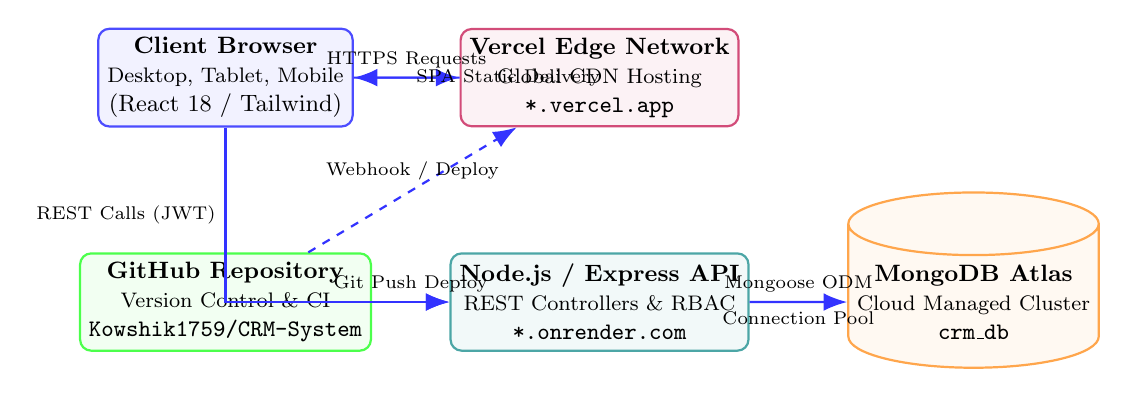
\begin{tikzpicture}[
    scale=0.95, every node/.style={transform shape},
    box/.style={rectangle, draw=blue!70, fill=blue!5, thick, rounded corners, minimum width=3.4cm, minimum height=1.3cm, align=center, font=\small},
    nodeBox/.style={rectangle, draw=teal!70, fill=teal!5, thick, rounded corners, minimum width=3.4cm, minimum height=1.3cm, align=center, font=\small},
    dbBox/.style={cylinder, draw=orange!70, fill=orange!5, shape border rotate=90, aspect=0.25, thick, minimum width=3.2cm, minimum height=1.5cm, align=center, font=\small},
    cloudBox/.style={rectangle, draw=gray!60, fill=gray!5, dashed, rounded corners, inner sep=12pt},
    arrow/.style={-{Latex[length=3mm]}, thick, draw=blue!80}
]

% Client Devices
\node[box] (browser) at (0, 4.5) {\textbf{Client Browser}\\\footnotesize Desktop, Tablet, Mobile\\(React 18 / Tailwind)};
\node[box, fill=purple!5, draw=purple!70] (vercel) at (5, 4.5) {\textbf{Vercel Edge Network}\\\footnotesize Global CDN Hosting\\\texttt{*.vercel.app}};

% Backend Server
\node[nodeBox] (api) at (5, 1.5) {\textbf{Node.js / Express API}\\\footnotesize REST Controllers \& RBAC\\\texttt{*.onrender.com}};

% Database
\node[dbBox] (mongo) at (10, 1.5) {\textbf{MongoDB Atlas}\\\footnotesize Cloud Managed Cluster\\\texttt{crm\_db}};

% DevOps & Delivery
\node[box, fill=green!5, draw=green!70] (github) at (0, 1.5) {\textbf{GitHub Repository}\\\footnotesize Version Control \& CI\\\texttt{Kowshik1759/CRM-System}};

% Flow Arrows
\draw[arrow] (browser) -- node[above, font=\scriptsize] {HTTPS Requests} (vercel);
\draw[arrow] (vercel) -- node[right, font=\scriptsize] {SPA Static Delivery} (browser);
\draw[arrow] (browser) |- node[near start, left, font=\scriptsize] {REST Calls (JWT)} (api);
\draw[arrow] (api) -- node[above, font=\scriptsize] {Mongoose ODM} node[below, font=\scriptsize] {Connection Pool} (mongo);
\draw[arrow, dashed] (github) -- node[above, font=\scriptsize] {Webhook / Deploy} (vercel);
\draw[arrow, dashed] (github) -- node[above, font=\scriptsize] {Git Push Deploy} (api);

\end{tikzpicture}
\caption{Overall High-Level System Architecture and Cloud Topology}
\label{fig:overall_architecture}
\end{figure}

\section{Three-Tier Architecture}
The CRM System adheres strictly to the classic Three-Tier Architectural model described by Fowler~\cite{fowler2002patterns}, cleanly segregating concerns across Presentation, Application Logic, and Data Storage tiers (Figure~\ref{fig:three_tier}).

\begin{figure}[h!]
\centering
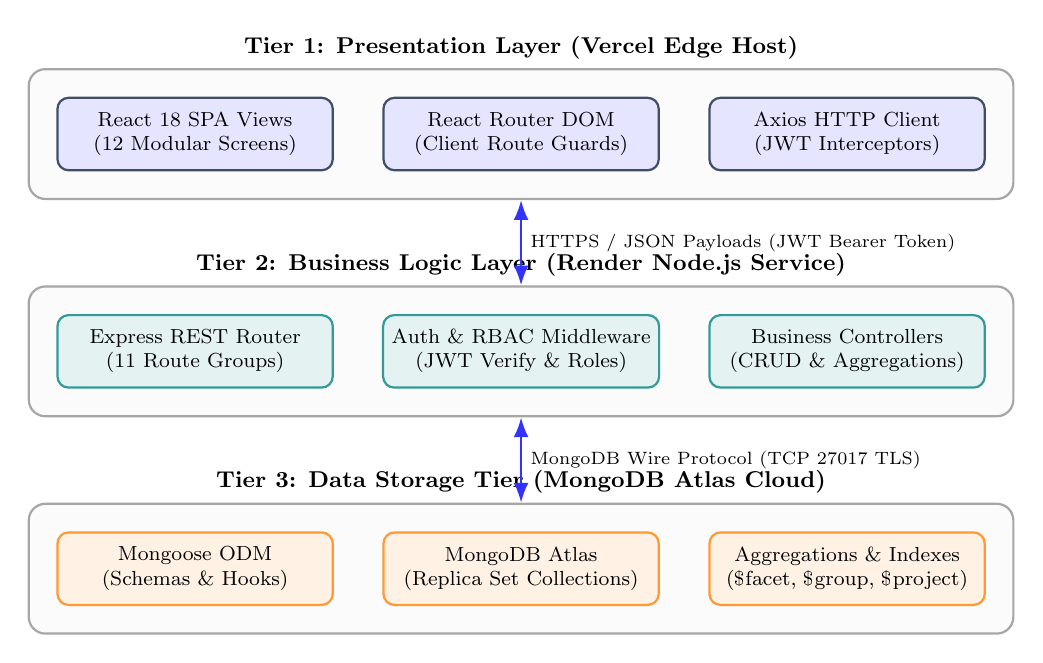
\begin{tikzpicture}[
    scale=0.92, every node/.style={transform shape},
    tierBox/.style={rectangle, draw=gray!70, fill=gray!3, thick, rounded corners=6pt, inner sep=10pt},
    comp/.style={rectangle, draw=navy!80, fill=blue!10, rounded corners=4pt, thick, minimum width=3.8cm, minimum height=1cm, align=center, font=\footnotesize},
    arrow/.style={{Latex[length=2.5mm]}-{Latex[length=2.5mm]}, thick, draw=blue!80}
]

% Tier 1: Presentation
\node[comp] (ui1) at (0, 6) {React 18 SPA Views\\(12 Modular Screens)};
\node[comp] (ui2) at (4.5, 6) {React Router DOM\\(Client Route Guards)};
\node[comp] (ui3) at (9, 6) {Axios HTTP Client\\(JWT Interceptors)};
\begin{scope}[on background layer]
    \node[tierBox, fit=(ui1) (ui3), label={[font=\small\bfseries]above:Tier 1: Presentation Layer (Vercel Edge Host)}] (tier1) {};
\end{scope}

% Tier 2: Application Logic
\node[comp, fill=teal!10, draw=teal!80] (srv1) at (0, 3) {Express REST Router\\(11 Route Groups)};
\node[comp, fill=teal!10, draw=teal!80] (srv2) at (4.5, 3) {Auth \& RBAC Middleware\\(JWT Verify \& Roles)};
\node[comp, fill=teal!10, draw=teal!80] (srv3) at (9, 3) {Business Controllers\\(CRUD \& Aggregations)};
\begin{scope}[on background layer]
    \node[tierBox, fit=(srv1) (srv3), label={[font=\small\bfseries]above:Tier 2: Business Logic Layer (Render Node.js Service)}] (tier2) {};
\end{scope}

% Tier 3: Data Tier
\node[comp, fill=orange!10, draw=orange!80] (db1) at (0, 0) {Mongoose ODM\\(Schemas \& Hooks)};
\node[comp, fill=orange!10, draw=orange!80] (db2) at (4.5, 0) {MongoDB Atlas\\(Replica Set Collections)};
\node[comp, fill=orange!10, draw=orange!80] (db3) at (9, 0) {Aggregations \& Indexes\\(\$facet, \$group, \$project)};
\begin{scope}[on background layer]
    \node[tierBox, fit=(db1) (db3), label={[font=\small\bfseries]above:Tier 3: Data Storage Tier (MongoDB Atlas Cloud)}] (tier3) {};
\end{scope}

% Connectors
\draw[arrow] (tier1.south) -- node[right, font=\scriptsize] {HTTPS / JSON Payloads (JWT Bearer Token)} (tier2.north);
\draw[arrow] (tier2.south) -- node[right, font=\scriptsize] {MongoDB Wire Protocol (TCP 27017 TLS)} (tier3.north);

\end{tikzpicture}
\caption{Three-Tier Enterprise Web Architectural Model}
\label{fig:three_tier}
\end{figure}

\begin{itemize}
    \item \textbf{Presentation Tier (Client):} Engineered as a single-page application (SPA) with React 18, Vite, and Tailwind CSS. It manages local component state, renders accessible user interfaces, enforces client route guards, and communicates with the backend via Axios interceptors.
    \item \textbf{Application Logic Tier (Server):} Implemented using Node.js and Express.js. It encapsulates stateless business rules, input validation, role-based authorization gates, cryptographic hashing, and RESTful routing.
    \item \textbf{Data Tier (Database):} Managed through MongoDB Atlas. It enforces data integrity via Mongoose schemas, manages relational document references, executes multi-stage analytical aggregations, and provides automated high availability.
\end{itemize}

\section{Frontend Architecture}
The frontend React architecture follows a component-driven design pattern:
\begin{itemize}
    \item \textbf{Context State Providers:} \texttt{AuthContext.jsx} maintains global user state, login tokens, and active permissions; \texttt{ToastContext.jsx} provides non-blocking visual feedback for mutations.
    \item \textbf{Route Guarding Shell:} \texttt{ProtectedRoute.jsx} wraps private routes, inspecting user authentication tokens and role allowances before allowing DOM mounting.
    \item \textbf{Shared Layout:} \texttt{DashboardLayout.jsx} houses the collapsible \texttt{Sidebar.jsx} and responsive \texttt{TopNavbar.jsx}, ensuring visual continuity across all twelve screens.
    \item \textbf{Modular API Client:} \texttt{axiosClient.js} establishes a centralized Axios instance configured with automatic \texttt{Bearer} token injection and response interceptors handling 401 session expiration redirects.
\end{itemize}

\section{Backend Architecture}
The Express.js backend is structured into modular layers adhering to separation of concerns:
\begin{itemize}
    \item \textbf{Server Entry (\texttt{server.js}):} Configures Express middleware (JSON body parsing, CORS, Morgan request logging), registers route modules, binds error handlers, and invokes database bootstrap routines.
    \item \textbf{Route Handlers (\texttt{routes/}):} Map incoming HTTP verbs and endpoints to specific controller functions, injecting \texttt{protect} and \texttt{authorize} middleware.
    \item \textbf{Business Controllers (\texttt{controllers/}):} Implement transactional logic, query formation, input sanitization, error propagation, and HTTP response formatting.
    \item \textbf{Data Models (\texttt{models/}):} Define strict Mongoose schemas with validation constraints, pre-save cryptographic hooks, compound indexes, and virtual references.
\end{itemize}

\section{Database Architecture}
The persistence tier uses MongoDB Atlas, a cloud-hosted distributed document database. Collections are structured with relational Object-Id cross-references (e.g., linking a \texttt{Lead} or \texttt{Opportunity} to an assigned \texttt{User} and converted \texttt{Customer}). Indexing strategies ensure fast query execution:
\begin{itemize}
    \item Unique index on \texttt{User.email} and \texttt{Customer.email}.
    \item Single-field indexes on \texttt{assignedTo}, \texttt{status}, \texttt{stage}, and \texttt{dueDate}.
    \item Compound index on \texttt{\{ customer: 1, createdAt: -1 \}} for chronological interaction timeline retrieval.
\end{itemize}

\section{System Workflow}
The operational lifecycle within the CRM commences with secure user authentication. Once verified, the user is transitioned to their designated landing screen based on their role. A Sales Executive processes incoming leads, progresses opportunities across the Kanban pipeline, schedules follow-up calls, delegates operational tasks, and documents interactions. Simultaneously, Sales Managers review real-time conversion rates and assign unallocated leads, while Administrators oversee employee accounts and audit reports.

\section{Use Case Diagram}
Figure~\ref{fig:use_case} details the system use case diagram, mapping interactions between the four primary actors and the functional use cases.

\begin{figure}[h!]
\centering
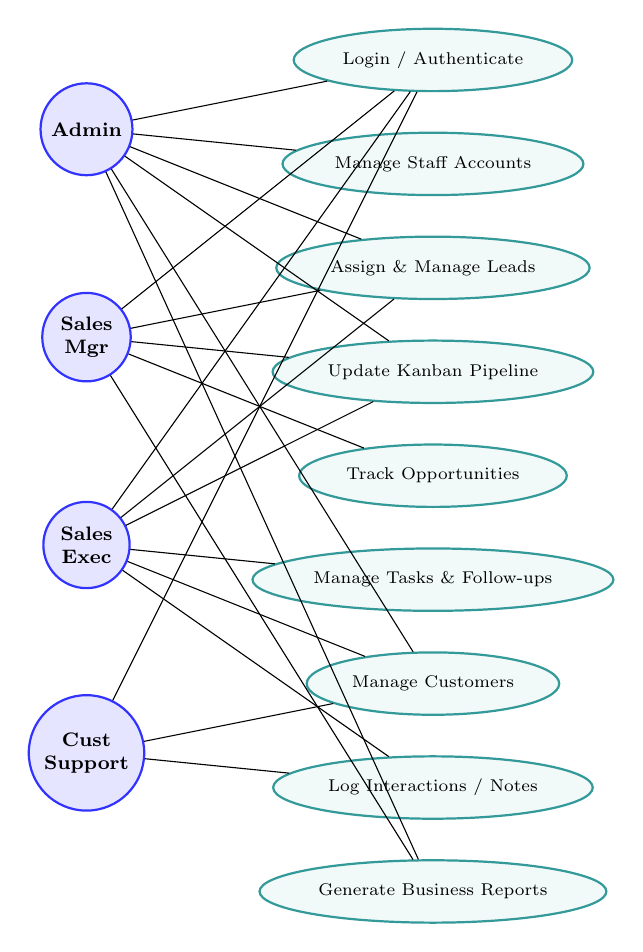
\begin{tikzpicture}[
    scale=0.88, every node/.style={transform shape},
    actor/.style={circle, draw=blue!80, fill=blue!10, thick, minimum size=1cm, font=\bfseries\footnotesize, align=center},
    uc/.style={ellipse, draw=teal!80, fill=teal!5, thick, minimum width=3.4cm, minimum height=0.9cm, align=center, font=\scriptsize}
]

% Actors
\node[actor] (admin) at (-4, 5) {Admin};
\node[actor] (mgr) at (-4, 2) {Sales\\Mgr};
\node[actor] (exec) at (-4, -1) {Sales\\Exec};
\node[actor] (supp) at (-4, -4) {Cust\\Support};

% Use Cases
\node[uc] (uc_login) at (1, 6) {Login / Authenticate};
\node[uc] (uc_users) at (1, 4.5) {Manage Staff Accounts};
\node[uc] (uc_leads) at (1, 3) {Assign \& Manage Leads};
\node[uc] (uc_pipe) at (1, 1.5) {Update Kanban Pipeline};
\node[uc] (uc_opps) at (1, 0) {Track Opportunities};
\node[uc] (uc_tasks) at (1, -1.5) {Manage Tasks \& Follow-ups};
\node[uc] (uc_cust) at (1, -3) {Manage Customers};
\node[uc] (uc_inter) at (1, -4.5) {Log Interactions / Notes};
\node[uc] (uc_reps) at (1, -6) {Generate Business Reports};

% Connections: Admin (has access to all)
\draw (admin) -- (uc_login);
\draw (admin) -- (uc_users);
\draw (admin) -- (uc_leads);
\draw (admin) -- (uc_pipe);
\draw (admin) -- (uc_cust);
\draw (admin) -- (uc_reps);

% Connections: Sales Manager
\draw (mgr) -- (uc_login);
\draw (mgr) -- (uc_leads);
\draw (mgr) -- (uc_pipe);
\draw (mgr) -- (uc_opps);
\draw (mgr) -- (uc_reps);

% Connections: Sales Executive
\draw (exec) -- (uc_login);
\draw (exec) -- (uc_leads);
\draw (exec) -- (uc_pipe);
\draw (exec) -- (uc_tasks);
\draw (exec) -- (uc_cust);
\draw (exec) -- (uc_inter);

% Connections: Customer Support
\draw (supp) -- (uc_login);
\draw (supp) -- (uc_cust);
\draw (supp) -- (uc_inter);

\end{tikzpicture}
\caption{UML Use Case Diagram Illustrating Multi-Actor Permissions}
\label{fig:use_case}
\end{figure}

\section{Data Flow Diagram -- Level 0}
Figure~\ref{fig:dfd_level0} illustrates the Context Diagram (DFD Level 0), modeling information flows across external actors and the centralized CRM System.

\begin{figure}[h!]
\centering
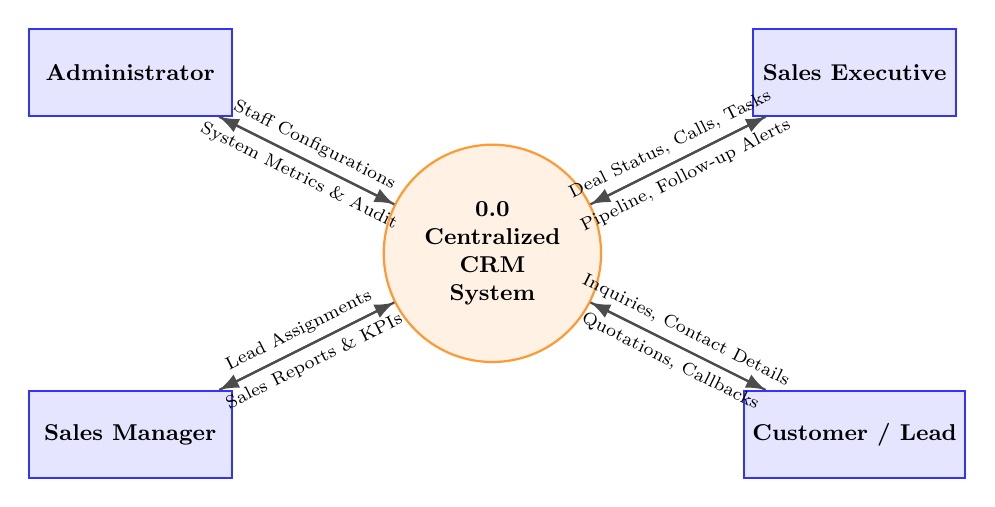
\begin{tikzpicture}[
    scale=0.92, every node/.style={transform shape},
    entity/.style={rectangle, draw=blue!80, fill=blue!10, thick, minimum width=2.8cm, minimum height=1.2cm, align=center, font=\small\bfseries},
    proc/.style={circle, draw=orange!80, fill=orange!10, thick, minimum size=3cm, align=center, font=\small\bfseries},
    arrow/.style={-{Latex[length=2.5mm]}, thick, draw=black!70}
]

\node[proc] (crm) at (0, 0) {0.0\\Centralized\\CRM\\System};

\node[entity] (admin) at (-5, 2.5) {Administrator};
\node[entity] (mgr) at (-5, -2.5) {Sales Manager};
\node[entity] (exec) at (5, 2.5) {Sales Executive};
\node[entity] (client) at (5, -2.5) {Customer / Lead};

\draw[arrow] (admin) -- node[above, sloped, font=\scriptsize] {Staff Configurations} (crm);
\draw[arrow] (crm) -- node[below, sloped, font=\scriptsize] {System Metrics \& Audit} (admin);

\draw[arrow] (mgr) -- node[above, sloped, font=\scriptsize] {Lead Assignments} (crm);
\draw[arrow] (crm) -- node[below, sloped, font=\scriptsize] {Sales Reports \& KPIs} (mgr);

\draw[arrow] (exec) -- node[above, sloped, font=\scriptsize] {Deal Status, Calls, Tasks} (crm);
\draw[arrow] (crm) -- node[below, sloped, font=\scriptsize] {Pipeline, Follow-up Alerts} (exec);

\draw[arrow] (client) -- node[above, sloped, font=\scriptsize] {Inquiries, Contact Details} (crm);
\draw[arrow] (crm) -- node[below, sloped, font=\scriptsize] {Quotations, Callbacks} (client);

\end{tikzpicture}
\caption{Data Flow Diagram Level 0 (Context-Level Diagram)}
\label{fig:dfd_level0}
\end{figure}

\section{Data Flow Diagram -- Level 1}
Figure~\ref{fig:dfd_level1} decomposes the CRM into core processes and underlying data stores.

\begin{figure}[h!]
\centering
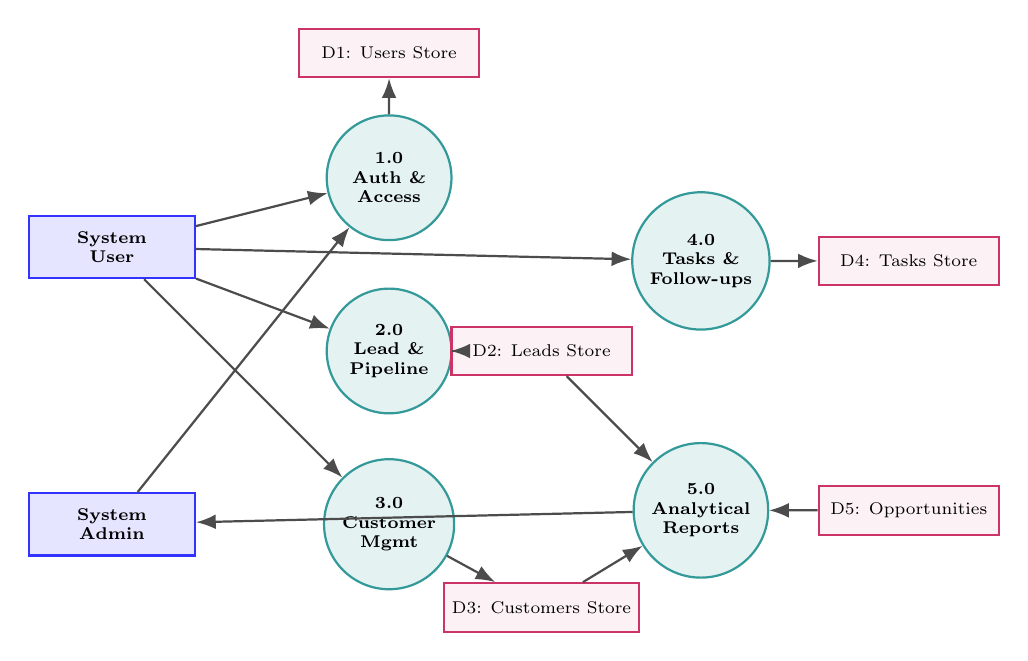
\begin{tikzpicture}[
    scale=0.88, every node/.style={transform shape},
    proc/.style={circle, draw=teal!80, fill=teal!10, thick, minimum size=1.8cm, align=center, font=\scriptsize\bfseries},
    dstore/.style={rectangle, draw=purple!80, fill=purple!5, thick, minimum width=2.6cm, minimum height=0.7cm, align=center, font=\scriptsize},
    ext/.style={rectangle, draw=blue!80, fill=blue!10, thick, minimum width=2.4cm, minimum height=0.9cm, align=center, font=\scriptsize\bfseries},
    arrow/.style={-{Latex[length=2.5mm]}, thick, draw=black!70}
]

% External entities
\node[ext] (user) at (-5, 2) {System\\User};
\node[ext] (admin) at (-5, -2) {System\\Admin};

% Processes
\node[proc] (p1) at (-1, 3) {1.0\\Auth \&\\Access};
\node[proc] (p2) at (-1, 0.5) {2.0\\Lead \&\\Pipeline};
\node[proc] (p3) at (-1, -2) {3.0\\Customer\\Mgmt};
\node[proc] (p4) at (3.5, 1.8) {4.0\\Tasks \&\\Follow-ups};
\node[proc] (p5) at (3.5, -1.8) {5.0\\Analytical\\Reports};

% Data stores
\node[dstore] (d1) at (-1, 4.8) {D1: Users Store};
\node[dstore] (d2) at (1.2, 0.5) {D2: Leads Store};
\node[dstore] (d3) at (1.2, -3.2) {D3: Customers Store};
\node[dstore] (d4) at (6.5, 1.8) {D4: Tasks Store};
\node[dstore] (d5) at (6.5, -1.8) {D5: Opportunities};

% Connections
\draw[arrow] (user) -- (p1);
\draw[arrow] (p1) -- (d1);
\draw[arrow] (user) -- (p2);
\draw[arrow] (p2) -- (d2);
\draw[arrow] (user) -- (p3);
\draw[arrow] (p3) -- (d3);
\draw[arrow] (user) -- (p4);
\draw[arrow] (p4) -- (d4);
\draw[arrow] (d2) -- (p5);
\draw[arrow] (d3) -- (p5);
\draw[arrow] (d5) -- (p5);
\draw[arrow] (admin) -- (p1);
\draw[arrow] (p5) -- (admin);

\end{tikzpicture}
\caption{Data Flow Diagram Level 1 (Functional Decomposition)}
\label{fig:dfd_level1}
\end{figure}

\section{Entity Relationship Diagram}
Figure~\ref{fig:erd_diagram} displays the logical entity-relationship schema among the seven core MongoDB document collections.

\begin{figure}[h!]
\centering
\begin{tikzpicture}[
    scale=0.85, every node/.style={transform shape},
    entity/.style={rectangle, draw=navy!80, fill=blue!8, thick, rounded corners=2pt, minimum width=3.8cm, align=left, font=\scriptsize, inner sep=6pt},
    rel/.style={draw=black!70, thick, -{Latex[length=2.5mm]}}
]

\node[entity] (user) at (0, 4.5) {
\textbf{User (users)}\\
\hline
\underline{\_id}: ObjectId [PK]\\
name: String\\
email: String [Unique]\\
password: String [Hashed]\\
role: Enum [4 Roles]\\
department: String\\
isActive: Boolean
};

\node[entity] (cust) at (-5, 0.5) {
\textbf{Customer (customers)}\\
\hline
\underline{\_id}: ObjectId [PK]\\
name: String\\
email: String\\
phone: String\\
company: String\\
status: Enum\\
assignedTo: ObjectId [FK]\\
createdBy: ObjectId [FK]
};

\node[entity] (lead) at (5, 0.5) {
\textbf{Lead (leads)}\\
\hline
\underline{\_id}: ObjectId [PK]\\
name: String\\
company: String\\
source: Enum\\
stage: Enum [6 Stages]\\
expectedValue: Number\\
assignedTo: ObjectId [FK]\\
convertedCustId: ObjectId [FK]
};

\node[entity] (opp) at (5, -4) {
\textbf{Opportunity (opportunities)}\\
\hline
\underline{\_id}: ObjectId [PK]\\
title: String\\
value: Number\\
probability: Number\\
stage: Enum [5 Stages]\\
customer: ObjectId [FK]\\
assignedTo: ObjectId [FK]
};

\node[entity] (task) at (-5, -4) {
\textbf{Task (tasks)}\\
\hline
\underline{\_id}: ObjectId [PK]\\
title: String\\
priority: Enum [4 Levels]\\
status: Enum\\
dueDate: Date\\
assignedTo: ObjectId [FK]\\
customer: ObjectId [FK]
};

\node[entity] (follow) at (0, -1.8) {
\textbf{FollowUp (followups)}\\
\hline
\underline{\_id}: ObjectId [PK]\\
title: String\\
scheduledDate: Date\\
status: Enum\\
type: Enum\\
assignedTo: ObjectId [FK]\\
customer: ObjectId [FK]
};

% Relationships
\draw[rel] (user.west) -| node[above, near end, font=\tiny] {1 : N} (cust.north);
\draw[rel] (user.east) -| node[above, near end, font=\tiny] {1 : N} (lead.north);
\draw[rel] (user.south) -- node[right, font=\tiny] {1 : N} (follow.north);
\draw[rel] (cust.south) -- node[left, font=\tiny] {1 : N} (task.north);
\draw[rel] (lead.south) -- node[right, font=\tiny] {1 : N} (opp.north);
\draw[rel] (cust.east) -- node[above, font=\tiny] {1 : N} (follow.west);

\end{tikzpicture}
\caption{Entity-Relationship Diagram with MongoDB Foreign Key Object-Id References}
\label{fig:erd_diagram}
\end{figure}

\section{Database Design}
The database schemas for the seven collections implemented in Mongoose are defined in Tables~\ref{tab:schema_user} through~\ref{tab:schema_interaction}.

\begin{table}[h!]
\centering
\caption{Database Schema: \texttt{users} Collection}
\label{tab:schema_user}
\renewcommand{\arraystretch}{1.2}
\begin{tabular}{|p{3cm}|p{3cm}|p{3.5cm}|p{4.5cm}|}
\hline
\textbf{Field Name} & \textbf{Data Type} & \textbf{Constraints} & \textbf{Description} \\ \hline
\texttt{\_id} & ObjectId & Primary Key, Auto & Unique system document identifier \\ \hline
\texttt{name} & String & Required, Trimmed & Full name of the employee \\ \hline
\texttt{email} & String & Required, Unique, Lower & Corporate email address for login \\ \hline
\texttt{password} & String & Required, Min 6, Hidden & Bcrypt salted and hashed password \\ \hline
\texttt{role} & String & Enum, Default: \texttt{sales\_executive} & Role: admin, sales\_manager, sales\_executive, customer\_support \\ \hline
\texttt{phone} & String & Optional, Trimmed & Contact telephone number \\ \hline
\texttt{department} & String & Default: 'Sales' & Organizational operational department \\ \hline
\texttt{isActive} & Boolean & Default: \texttt{true} & Account status toggle for authentication \\ \hline
\texttt{createdAt} & Date & Auto Timestamp & System record generation timestamp \\ \hline
\end{tabular}
\end{table}

\begin{table}[h!]
\centering
\caption{Database Schema: \texttt{customers} Collection}
\label{tab:schema_customer}
\renewcommand{\arraystretch}{1.2}
\begin{tabular}{|p{3cm}|p{3cm}|p{3.5cm}|p{4.5cm}|}
\hline
\textbf{Field Name} & \textbf{Data Type} & \textbf{Constraints} & \textbf{Description} \\ \hline
\texttt{\_id} & ObjectId & Primary Key, Auto & Customer unique identifier \\ \hline
\texttt{name} & String & Required, Trimmed & Primary client contact name \\ \hline
\texttt{email} & String & Required, Unique & Primary business email address \\ \hline
\texttt{phone} & String & Required & Direct telephone contact number \\ \hline
\texttt{company} & String & Required & Name of the client commercial entity \\ \hline
\texttt{address} & String & Optional & Street address \\ \hline
\texttt{status} & String & Enum: \texttt{lead, active, inactive} & Current operational account state \\ \hline
\texttt{assignedTo} & ObjectId & Ref: \texttt{User} & Sales executive assigned to account \\ \hline
\texttt{createdBy} & ObjectId & Ref: \texttt{User} & User account who generated record \\ \hline
\end{tabular}
\end{table}

\begin{table}[h!]
\centering
\caption{Database Schema: \texttt{leads} Collection}
\label{tab:schema_lead}
\renewcommand{\arraystretch}{1.2}
\begin{tabular}{|p{3cm}|p{3cm}|p{3.5cm}|p{4.5cm}|}
\hline
\textbf{Field Name} & \textbf{Data Type} & \textbf{Constraints} & \textbf{Description} \\ \hline
\texttt{\_id} & ObjectId & Primary Key, Auto & Lead unique record identifier \\ \hline
\texttt{name} & String & Required, Trimmed & Prospective contact individual \\ \hline
\texttt{email} & String & Required & Inbound inquiry email \\ \hline
\texttt{company} & String & Required & Prospect commercial organization \\ \hline
\texttt{source} & String & Enum [Website, Referral, etc.] & Inbound channel origin \\ \hline
\texttt{stage} & String & Enum [6 Kanban Stages] & Pipeline qualification progress \\ \hline
\texttt{expectedValue}& Number & Default: 0, Min: 0 & Projected commercial contract value \\ \hline
\texttt{assignedTo} & ObjectId & Ref: \texttt{User} & Allocated sales representative \\ \hline
\texttt{convertedCustId}& ObjectId & Ref: \texttt{Customer}, Optional & ID of converted customer record \\ \hline
\end{tabular}
\end{table}

\begin{table}[h!]
\centering
\caption{Database Schema: \texttt{opportunities} Collection}
\label{tab:schema_opportunity}
\renewcommand{\arraystretch}{1.2}
\begin{tabular}{|p{3cm}|p{3cm}|p{3.5cm}|p{4.5cm}|}
\hline
\textbf{Field Name} & \textbf{Data Type} & \textbf{Constraints} & \textbf{Description} \\ \hline
\texttt{\_id} & ObjectId & Primary Key, Auto & Opportunity deal identifier \\ \hline
\texttt{title} & String & Required & Deal commercial headline \\ \hline
\texttt{value} & Number & Required, Min: 0 & Expected financial deal revenue \\ \hline
\texttt{probability} & Number & Min: 0, Max: 100 & Deal closing confidence percentage \\ \hline
\texttt{stage} & String & Enum [5 Stages] & Qualification to Closed Won/Lost \\ \hline
\texttt{customer} & ObjectId & Ref: \texttt{Customer} & Associated client account \\ \hline
\texttt{assignedTo} & ObjectId & Ref: \texttt{User} & Opportunity owner representative \\ \hline
\end{tabular}
\end{table}

\begin{table}[h!]
\centering
\caption{Database Schema: \texttt{tasks} Collection}
\label{tab:schema_task}
\renewcommand{\arraystretch}{1.2}
\begin{tabular}{|p{3cm}|p{3cm}|p{3.5cm}|p{4.5cm}|}
\hline
\textbf{Field Name} & \textbf{Data Type} & \textbf{Constraints} & \textbf{Description} \\ \hline
\texttt{\_id} & ObjectId & Primary Key, Auto & Task item unique identifier \\ \hline
\texttt{title} & String & Required & Task title and directive \\ \hline
\texttt{priority} & String & Enum: low, medium, high, urgent & Urgency escalation indicator \\ \hline
\texttt{status} & String & Enum: pending, completed, etc. & Work execution status \\ \hline
\texttt{dueDate} & Date & Required & Target deadline for completion \\ \hline
\texttt{assignedTo} & ObjectId & Ref: \texttt{User} & Designated employee assignee \\ \hline
\end{tabular}
\end{table}

\begin{table}[h!]
\centering
\caption{Database Schema: \texttt{followups} Collection}
\label{tab:schema_followup}
\renewcommand{\arraystretch}{1.2}
\begin{tabular}{|p{3cm}|p{3cm}|p{3.5cm}|p{4.5cm}|}
\hline
\textbf{Field Name} & \textbf{Data Type} & \textbf{Constraints} & \textbf{Description} \\ \hline
\texttt{\_id} & ObjectId & Primary Key, Auto & Follow-up schedule identifier \\ \hline
\texttt{title} & String & Required & Purpose of scheduled contact \\ \hline
\texttt{scheduledDate}& Date & Required & Timestamp for callback/meeting \\ \hline
\texttt{type} & String & Enum: call, email, meeting, demo & Contact modality format \\ \hline
\texttt{status} & String & Enum: pending, completed, overdue & Activity adherence state \\ \hline
\texttt{customer} & ObjectId & Ref: \texttt{Customer} & Targeted client profile \\ \hline
\end{tabular}
\end{table}

\begin{table}[h!]
\centering
\caption{Database Schema: \texttt{interactions} Collection}
\label{tab:schema_interaction}
\renewcommand{\arraystretch}{1.2}
\begin{tabular}{|p{3cm}|p{3cm}|p{3.5cm}|p{4.5cm}|}
\hline
\textbf{Field Name} & \textbf{Data Type} & \textbf{Constraints} & \textbf{Description} \\ \hline
\texttt{\_id} & ObjectId & Primary Key, Auto & Historical interaction log entry \\ \hline
\texttt{type} & String & Enum: call, meeting, email, note & Interaction channel format \\ \hline
\texttt{subject} & String & Required & Brief topic of client discussion \\ \hline
\texttt{details} & String & Required & Detailed discussion notes \\ \hline
\texttt{performedBy} & ObjectId & Ref: \texttt{User} & Employee who executed contact \\ \hline
\texttt{customer} & ObjectId & Ref: \texttt{Customer} & Associated client account \\ \hline
\end{tabular}
\end{table}

\section{UML Activity Diagram}
Figure~\ref{fig:activity_lead} demonstrates the operational activity workflow of a prospective lead from initial capture to customer conversion.

\begin{figure}[h!]
\centering
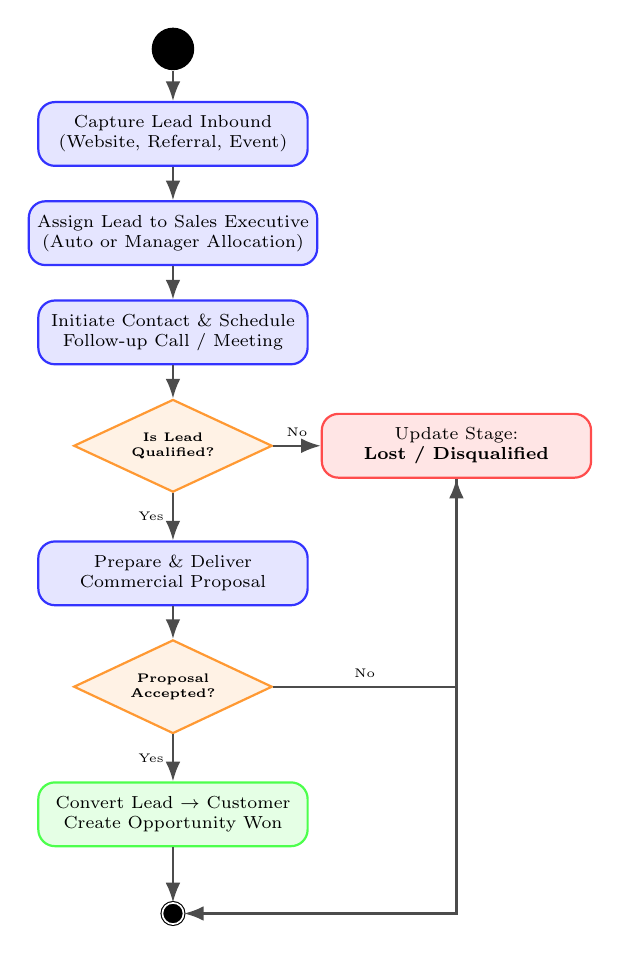
\begin{tikzpicture}[
    scale=0.9, every node/.style={transform shape},
    startStop/.style={circle, fill=black, minimum size=0.6cm},
    action/.style={rectangle, draw=blue!80, fill=blue!10, rounded corners=6pt, thick, minimum width=3.8cm, minimum height=0.9cm, align=center, font=\scriptsize},
    decision/.style={diamond, draw=orange!80, fill=orange!10, thick, aspect=2, minimum width=2.8cm, align=center, font=\tiny\bfseries},
    arrow/.style={-{Latex[length=2.5mm]}, thick, draw=black!70}
]

\node[startStop] (start) at (0, 7) {};
\node[action] (a1) at (0, 5.8) {Capture Lead Inbound\\(Website, Referral, Event)};
\node[action] (a2) at (0, 4.4) {Assign Lead to Sales Executive\\(Auto or Manager Allocation)};
\node[action] (a3) at (0, 3.0) {Initiate Contact \& Schedule\\Follow-up Call / Meeting};
\node[decision] (d1) at (0, 1.4) {Is Lead\\Qualified?};
\node[action, fill=red!10, draw=red!70] (lost) at (4, 1.4) {Update Stage:\\\textbf{Lost / Disqualified}};
\node[action] (a4) at (0, -0.4) {Prepare \& Deliver\\Commercial Proposal};
\node[decision] (d2) at (0, -2.0) {Proposal\\Accepted?};
\node[action, fill=green!10, draw=green!70] (win) at (0, -3.8) {Convert Lead $\rightarrow$ Customer\\Create Opportunity Won};
\node[circle, draw=black, double, inner sep=3pt, fill=black] (finish) at (0, -5.2) {};

% Flows
\draw[arrow] (start) -- (a1);
\draw[arrow] (a1) -- (a2);
\draw[arrow] (a2) -- (a3);
\draw[arrow] (a3) -- (d1);
\draw[arrow] (d1) -- node[above, font=\tiny] {No} (lost);
\draw[arrow] (d1) -- node[left, font=\tiny] {Yes} (a4);
\draw[arrow] (a4) -- (d2);
\draw[arrow] (d2) -| node[above, near start, font=\tiny] {No} (lost);
\draw[arrow] (d2) -- node[left, font=\tiny] {Yes} (win);
\draw[arrow] (win) -- (finish);
\draw[arrow] (lost) |- (finish);

\end{tikzpicture}
\caption{UML Activity Diagram: Complete Commercial Lead Lifecycle}
\label{fig:activity_lead}
\end{figure}

\section{Sequence Diagram}
Figure~\ref{fig:sequence_login} illustrates the sequence of interactions among the Client Browser, Axios Interceptor, Express Auth Router, and MongoDB Atlas during user authentication.

\begin{figure}[h!]
\centering
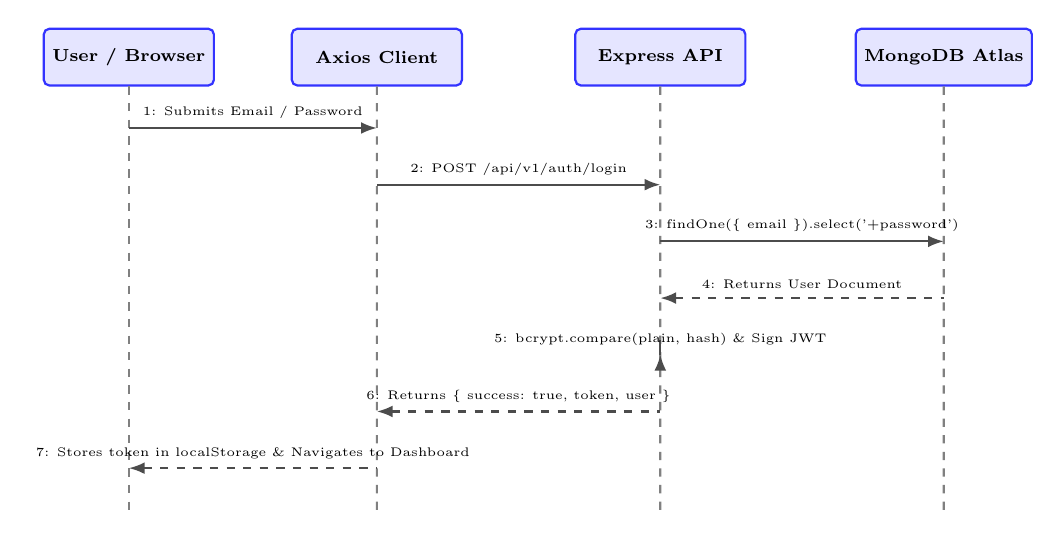
\begin{tikzpicture}[
    scale=0.9, every node/.style={transform shape},
    lifeline/.style={draw=black!50, dashed, thick},
    actorBox/.style={rectangle, draw=blue!80, fill=blue!10, thick, rounded corners=2pt, minimum width=2.4cm, minimum height=0.8cm, align=center, font=\scriptsize\bfseries},
    msg/.style={-{Latex[length=2mm]}, thick, draw=black!70, font=\tiny},
    reply/.style={{Latex[length=2mm]}-, dashed, thick, draw=black!70, font=\tiny}
]

% Lifeline headers
\node[actorBox] (c) at (0, 0) {User / Browser};
\node[actorBox] (ax) at (3.5, 0) {Axios Client};
\node[actorBox] (api) at (7.5, 0) {Express API};
\node[actorBox] (db) at (11.5, 0) {MongoDB Atlas};

% Lifelines
\draw[lifeline] (c) -- (0, -6.5);
\draw[lifeline] (ax) -- (3.5, -6.5);
\draw[lifeline] (api) -- (7.5, -6.5);
\draw[lifeline] (db) -- (11.5, -6.5);

% Messages
\draw[msg] (0, -1) -- node[above] {1: Submits Email / Password} (3.5, -1);
\draw[msg] (3.5, -1.8) -- node[above] {2: POST /api/v1/auth/login} (7.5, -1.8);
\draw[msg] (7.5, -2.6) -- node[above] {3: findOne(\{ email \}).select('+password')} (11.5, -2.6);
\draw[reply] (7.5, -3.4) -- node[above] {4: Returns User Document} (11.5, -3.4);
\draw[msg] (7.5, -4.2) -- node[above] {5: bcrypt.compare(plain, hash) \& Sign JWT} (7.5, -4.2);
\draw[reply] (3.5, -5.0) -- node[above] {6: Returns \{ success: true, token, user \}} (7.5, -5.0);
\draw[reply] (0, -5.8) -- node[above] {7: Stores token in localStorage \& Navigates to Dashboard} (3.5, -5.8);

\end{tikzpicture}
\caption{UML Sequence Diagram: Authentication and JWT Generation Protocol}
\label{fig:sequence_login}
\end{figure}

\section{Authentication Workflow}
The authentication workflow guarantees stateless identity verification. When a user submits credentials, the server retrieves the corresponding record, verifies the bcrypt hash, checks the \texttt{isActive} boolean flag, and generates a signed JWT payload containing \texttt{\{ id: user.\_id, role: user.role \}} with a 7-day expiration. The client caches the token in browser \texttt{localStorage} and mounts protected layout trees.

\section{Customer Management Workflow}
The Customer module permits authorized staff to maintain business accounts. When creating a customer, input validation checks unique email constraints. Modifications update the record timestamp, and delete requests are protected by a confirmation modal dialog, updating linked interactions.

\section{Lead Management Workflow}
Leads enter the system with a default stage of \textit{New}. A sales representative qualifies the prospect by capturing contact requirements, estimated value, and acquisition channel. Converting a lead generates a persistent customer document, updates the lead status to \textit{Converted}, and establishes an associated initial sales opportunity.

\section{Task Management Workflow}
Tasks facilitate team delegation. A manager or representative specifies a task title, priority, due date, and assigned employee. The system monitors upcoming deadlines, categorizes items dynamically into Pending, In Progress, or Completed states, and surfaces overdue task alerts on the central executive dashboard.


% Chapter 4: Implementation
\chapter{IMPLEMENTATION}

\section{Technology Stack}
The implementation of the CRM System leverages the MERN technology stack, incorporating modern industry frameworks, build tools, and software engineering libraries:
\begin{itemize}
    \item \textbf{Frontend:} React.js (v18.2.0) configured with Vite (v5.2.8) for fast module replacement, Tailwind CSS (v3.4.3) for styling, React Router DOM (v6.22.3) for single-page routing, Axios (v1.6.8) for HTTP networking, Lucide React (v0.364.0) for accessible icons, and Recharts (v2.12.3) for dynamic data visualization.
    \item \textbf{Backend:} Node.js (v20+ LTS) and Express.js (v4.19.2), structured as a REST API architecture utilizing JSON Web Tokens (\texttt{jsonwebtoken} v9.0.2) for stateless authentication, \texttt{bcryptjs} (v2.4.3) for cryptographic salt-and-hash operations, \texttt{cors} (v2.8.5) for cross-origin security, and \texttt{morgan} (v1.10.0) for HTTP transaction logging.
    \item \textbf{Database:} MongoDB Atlas cloud cluster connected through Mongoose ODM (v8.3.1), utilizing asynchronous connection pooling, schema validations, pre-save middleware hooks, relational document population, and multi-stage aggregation pipelines.
\end{itemize}

\section{Frontend Implementation}
The client application is built as an ergonomic Single Page Application (SPA). Global authentication state is managed via \texttt{AuthContext.jsx}, storing the active user profile and token in browser \texttt{localStorage} to ensure session persistence across browser reloads. Centralized Axios interceptors in \texttt{axiosClient.js} automatically inject the authorization bearer header into outgoing requests:

\begin{lstlisting}[language=JavaScript, caption={Axios Client Interceptors in \texttt{frontend/src/api/axiosClient.js}}]
import axios from 'axios';

const API_BASE_URL = import.meta.env.VITE_API_URL || '/api/v1';

const axiosClient = axios.create({
  baseURL: API_BASE_URL,
  headers: { 'Content-Type': 'application/json' }
});

// Request interceptor to attach JWT token
axiosClient.interceptors.request.use((config) => {
  const token = localStorage.getItem('crm_token');
  if (token) {
    config.headers.Authorization = `Bearer ${token}`;
  }
  return config;
});

// Response interceptor to handle unauthorized 401 errors
axiosClient.interceptors.response.use(
  (response) => response.data,
  (error) => {
    if (error.response && error.response.status === 401) {
      localStorage.removeItem('crm_token');
      localStorage.removeItem('crm_user');
      if (window.location.pathname !== '/login') {
        window.location.href = '/login?expired=true';
      }
    }
    return Promise.reject(new Error(error.response?.data?.message || 'Error'));
  }
);
\end{lstlisting}

\section{React Application Structure}
The frontend source code is organized into modular folders under \texttt{frontend/src/}:
\begin{itemize}
    \item \texttt{api/}: Centralized Axios client instance and endpoint constants.
    \item \texttt{components/}:
    \begin{itemize}
        \item \texttt{auth/}: \texttt{ProtectedRoute.jsx} protecting private routes by role.
        \item \texttt{common/}: Reusable UI widgets (\texttt{Badge.jsx}, \texttt{Modal.jsx}, \texttt{Pagination.jsx}, \texttt{ConfirmDialog.jsx}, \texttt{LoadingSkeleton.jsx}, \texttt{EmptyState.jsx}).
        \item \texttt{layout/}: Application frame consisting of \texttt{DashboardLayout.jsx}, \texttt{Sidebar.jsx}, and \texttt{TopNavbar.jsx}.
    \end{itemize}
    \item \texttt{context/}: \texttt{AuthContext.jsx} (state, login, logout, profile updates) and \texttt{ToastContext.jsx} (toast alerts).
    \item \texttt{pages/}: The twelve operational screen components.
\end{itemize}

\section{Login Page Implementation}
The \texttt{Login.jsx} component delivers an intuitive authentication portal. It provides direct single-click credential quick-fill cards for all four system roles (\textit{Admin, Sales Manager, Sales Executive, Customer Support}), an automated demo password fill mechanism, a remember-session checkbox, a password visibility toggle, and client-side form validation. Invalid credentials trigger red feedback alerts without corrupting browser state.

\begin{figure}[h!]
\centering
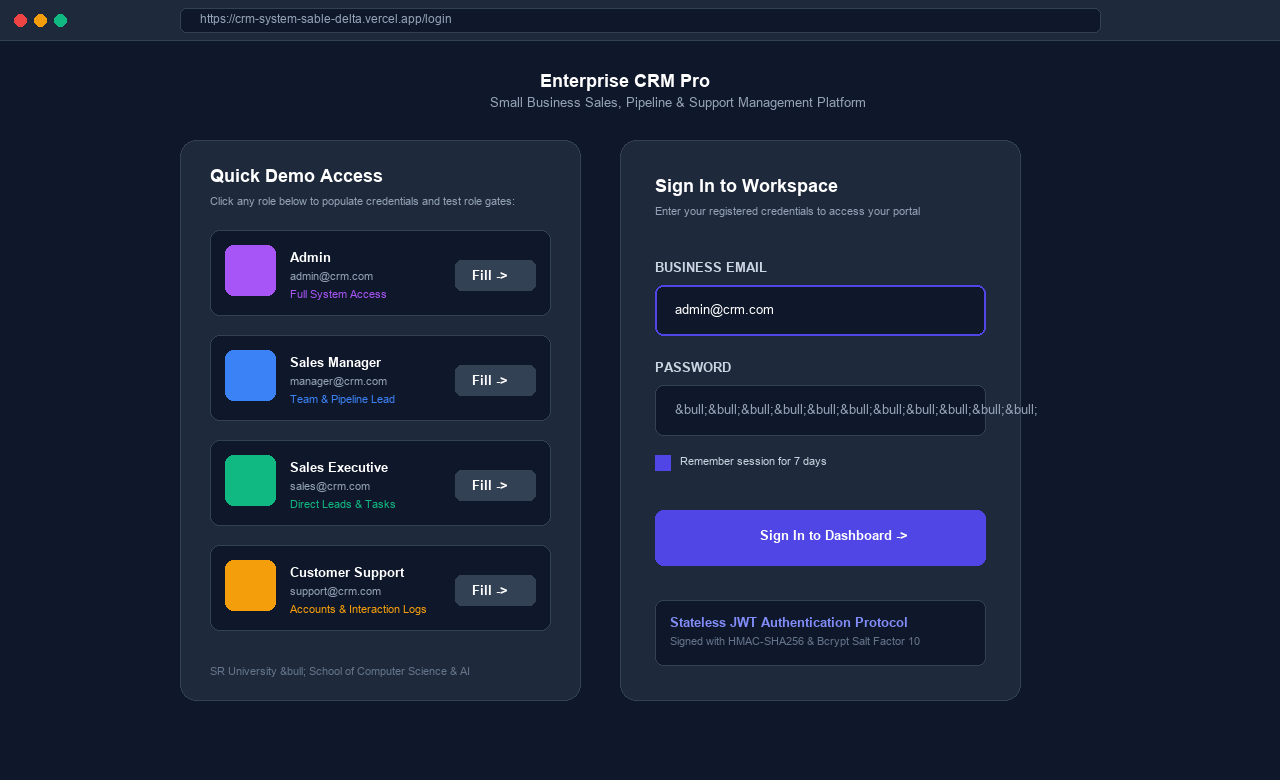
\includegraphics[width=0.95\textwidth]{figures/screen_login.png}
\caption{CRM Portal Authentication Interface with Multi-Role Demo Cards}
\label{fig:screen_login}
\end{figure}

\section{Dashboard Implementation}
The \texttt{Dashboard.jsx} screen acts as the operational nerve center. Upon mounting, it dispatches an asynchronous call to \texttt{/api/v1/dashboard}, retrieving:
\begin{enumerate}
    \item \textbf{KPI Summary Cards:} Total Customers, Active Leads in Pipeline, Closed Won Revenue, and Pending Follow-ups with percentage trend indicators.
    \item \textbf{Monthly Revenue Analytics:} An interactive Recharts area/bar chart displaying twelve-month revenue trends.
    \item \textbf{Lead Source Breakdown:} A Recharts pie chart categorizing lead acquisition channels (Website, Referrals, LinkedIn, Cold Calls).
    \item \textbf{Recent Activity Feeds:} Tabular widgets displaying recently logged interactions, impending tasks, and high-value opportunities.
\end{enumerate}

\begin{figure}[h!]
\centering
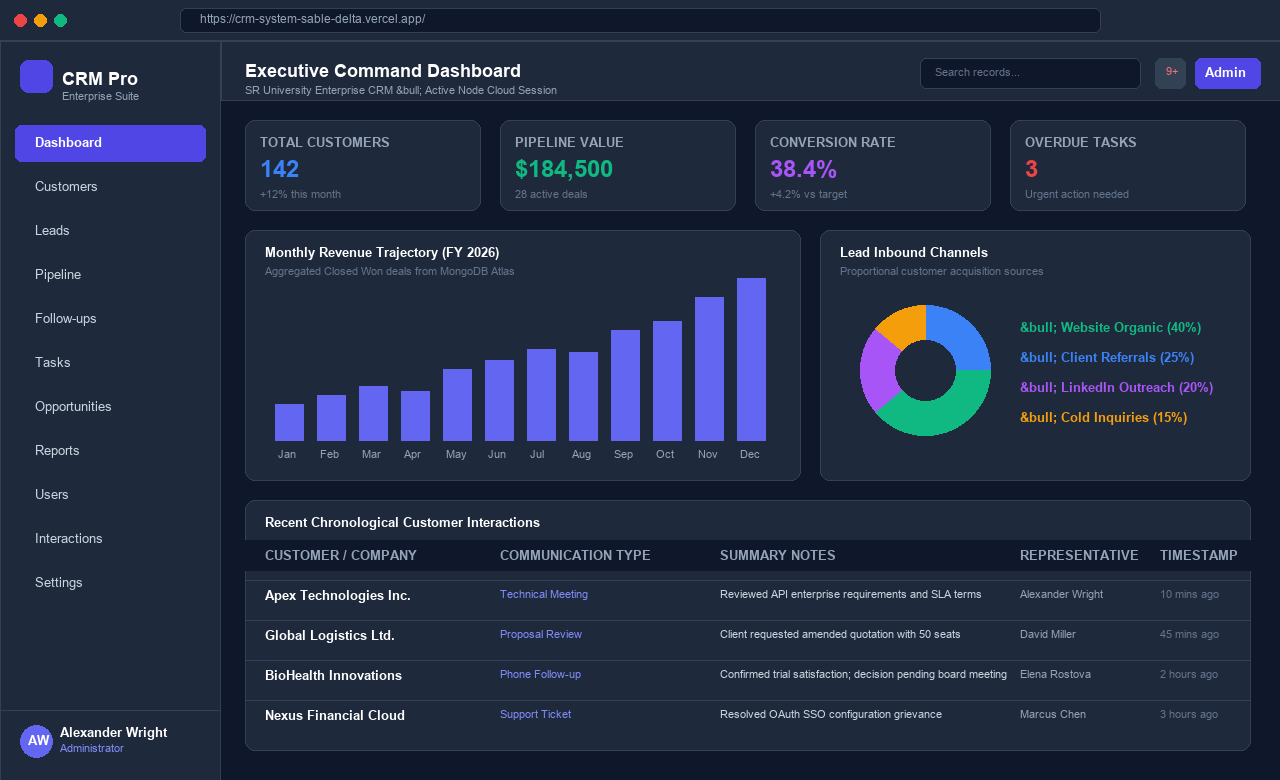
\includegraphics[width=0.95\textwidth]{figures/screen_dashboard.png}
\caption{Executive Command Dashboard Featuring Real-Time KPIs and Recharts Analytics}
\label{fig:screen_dashboard}
\end{figure}

\section{Customer Management Module}
The \texttt{Customers.jsx} page provides end-to-end account management. Users can search by customer name, company, or email, filter by account status (\textit{Lead, Active, Inactive}), and sort columns dynamically. Clicking ``Add Customer'' launches an accessible modal dialog containing field validations. Editing updates records via \texttt{PUT /api/v1/customers/:id}, and deletion triggers a secondary confirmation modal.

\begin{figure}[h!]
\centering
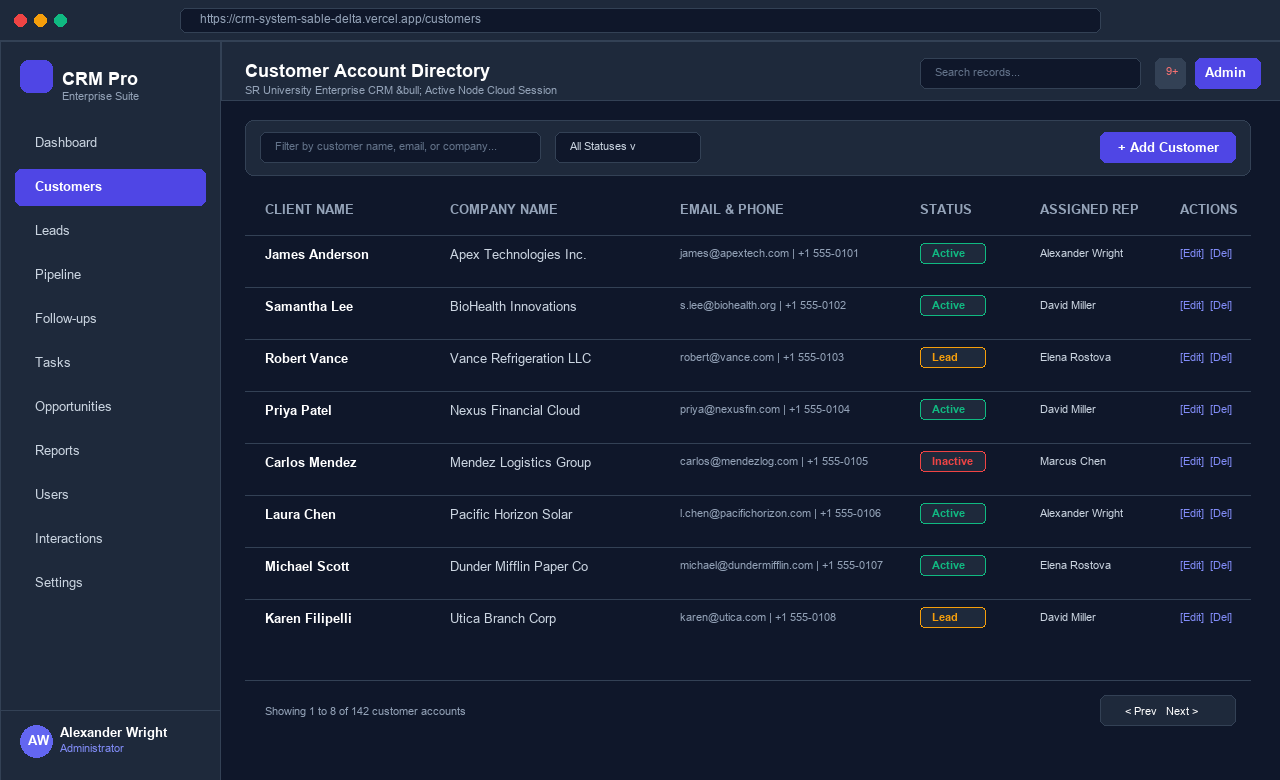
\includegraphics[width=0.95\textwidth]{figures/screen_customers.png}
\caption{Customer Account Management Directory with Multi-Criteria Search and Filtering}
\label{fig:screen_customers}
\end{figure}

\section{Lead Management Module}
The \texttt{Leads.jsx} module coordinates prospect ingestion and qualification. Each lead record captures the contact individual, company, lead source, assigned sales executive, estimated deal value, and priority score. A dedicated ``Convert to Customer'' action allows sales representatives to transition qualified prospects directly into the customer registry, automatically instantiating a connected customer record and closing the lead with zero data re-entry.

\begin{figure}[h!]
\centering
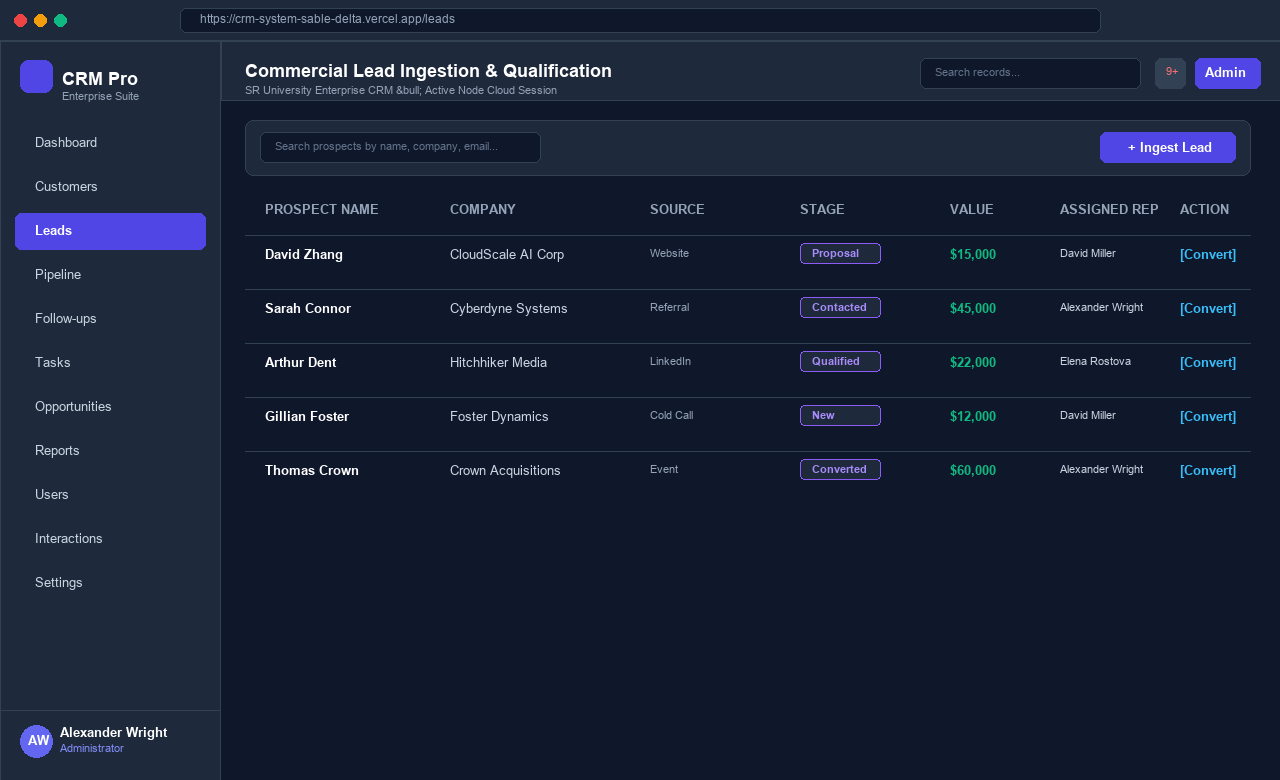
\includegraphics[width=0.95\textwidth]{figures/screen_leads.png}
\caption{Commercial Lead Ingestion, Qualification, and Conversion Module}
\label{fig:screen_leads}
\end{figure}

\section{Task Management Module}
The \texttt{Tasks.jsx} module organizes operational workflows. Tasks are categorized by priority level (\textit{Urgent, High, Medium, Low}) and status (\textit{Pending, In Progress, Completed, Deferred}). Visual badge indicators highlight overdue tasks whose deadlines have elapsed, and direct completion checkboxes trigger non-blocking API status updates.

\begin{figure}[h!]
\centering
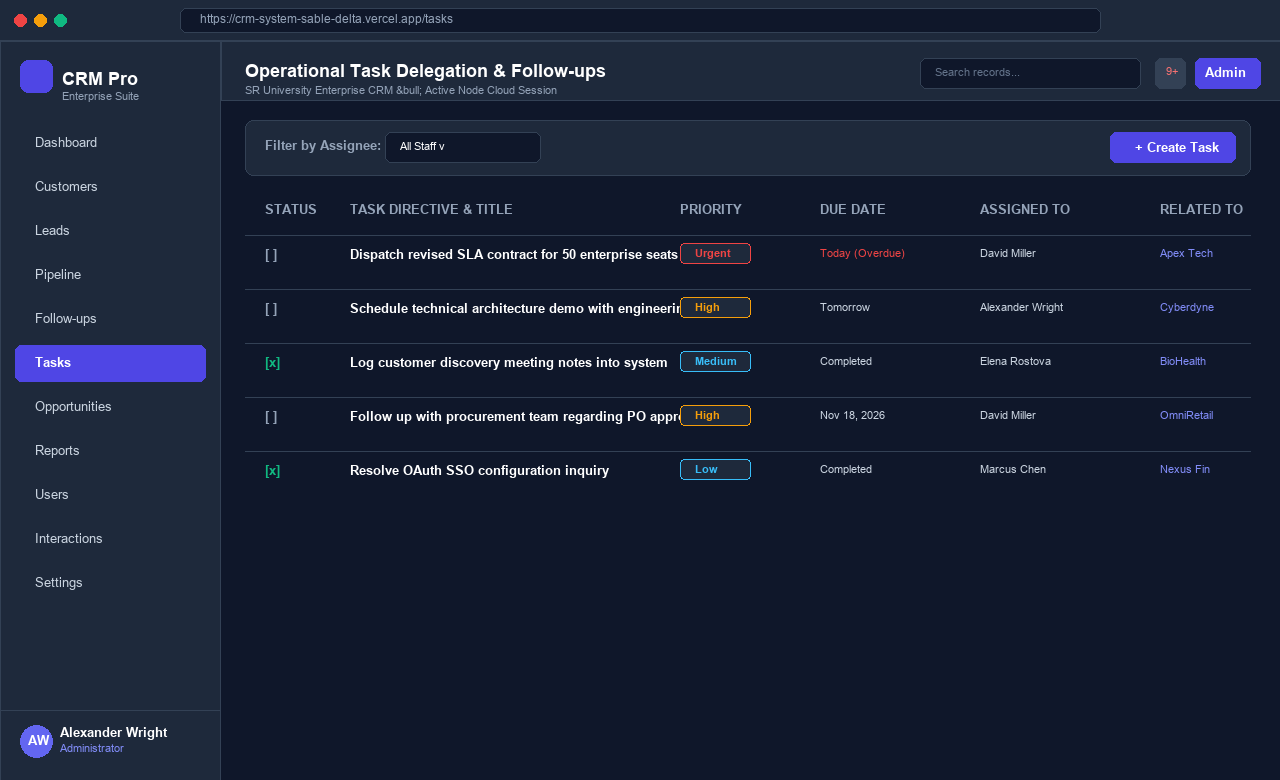
\includegraphics[width=0.95\textwidth]{figures/screen_tasks.png}
\caption{Operational Task Delegation Board with Priority Badges and Deadline Tracking}
\label{fig:screen_tasks}
\end{figure}

\section{Visual Kanban Pipeline & Reporting Implementation}
The system delivers an interactive Kanban sales pipeline (\texttt{SalesPipeline.jsx}) allowing dynamic deal stage updates, and a comprehensive reporting suite (\texttt{Reports.jsx}) backed by MongoDB aggregations.

\begin{figure}[h!]
\centering
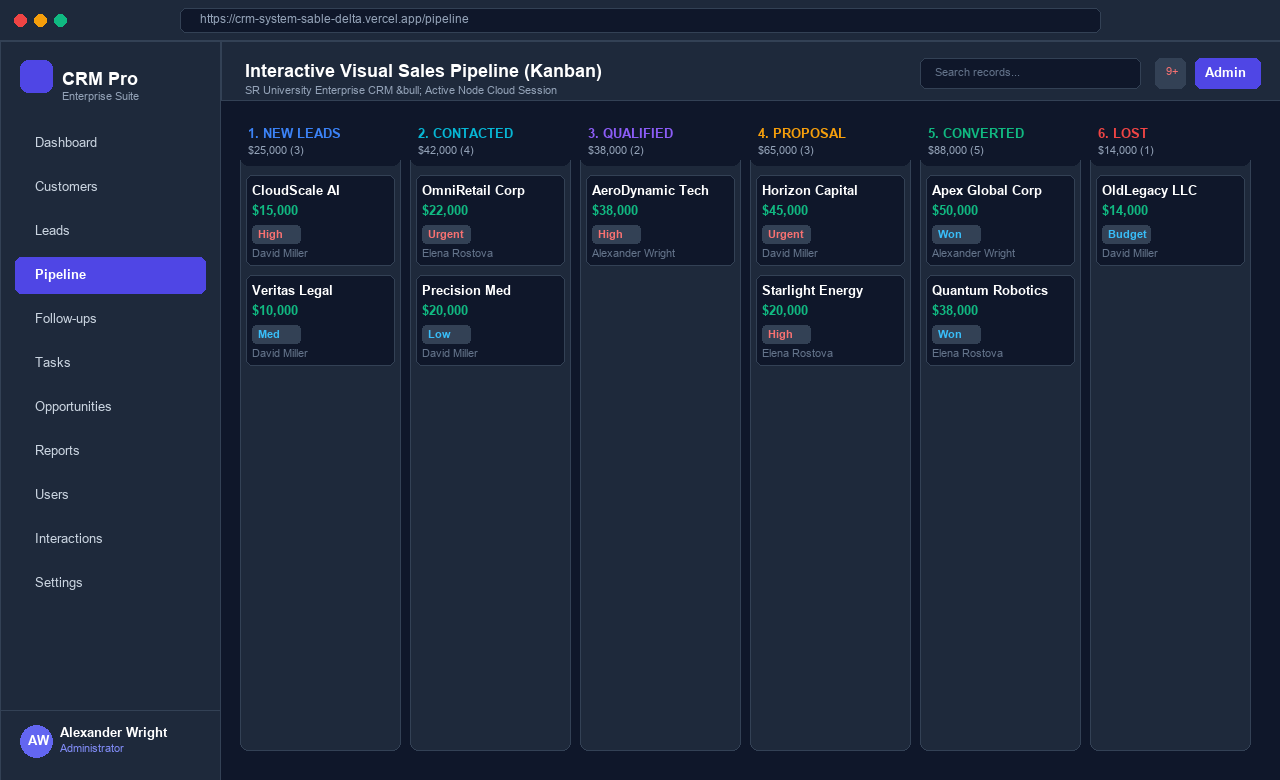
\includegraphics[width=0.95\textwidth]{figures/screen_pipeline.png}
\caption{Interactive Kanban Sales Pipeline with Six Stage-Gate Deal Columns}
\label{fig:screen_pipeline}
\end{figure}

\begin{figure}[h!]
\centering
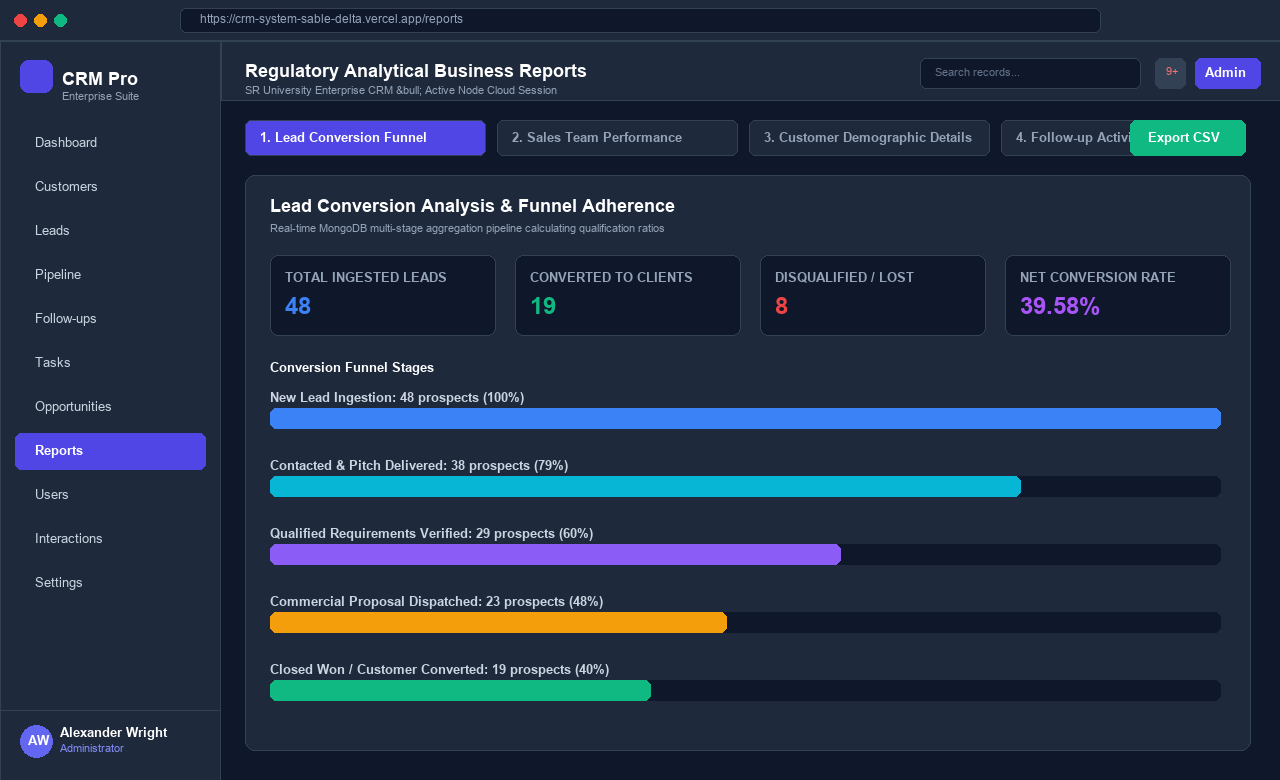
\includegraphics[width=0.95\textwidth]{figures/screen_reports.png}
\caption{Mandatory Analytical Reports Suite with Real-Time Conversion Funnel and CSV Export}
\label{fig:screen_reports}
\end{figure}

\begin{figure}[h!]
\centering
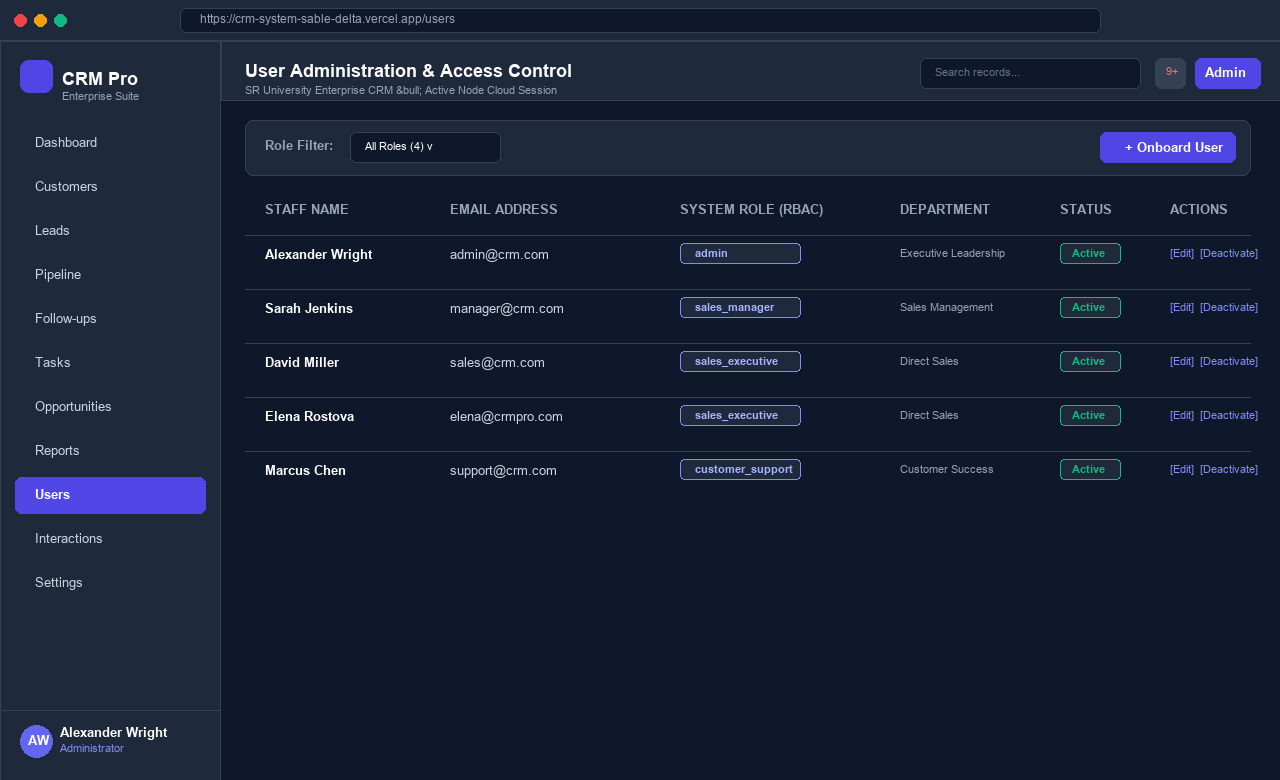
\includegraphics[width=0.95\textwidth]{figures/screen_users.png}
\caption{User Administration Console with Role-Based Access Control Boundaries}
\label{fig:screen_users}
\end{figure}

\section{Backend Implementation}
The backend server is implemented as an asynchronous Node.js Express service. In \texttt{server.js}, incoming requests are processed through body parsers, CORS handlers, route mappers, and an error interception pipeline. When starting up, the server invokes \texttt{connectDB()} to verify MongoDB Atlas connectivity, followed by an automatic bootstrap check: if the database has zero user records, the automated seeder (\texttt{seeder.js}) populates the cluster with system users, realistic customers, pipeline leads, and sample transactions.

\section{REST API Implementation}
Table~\ref{tab:api_endpoints} documents the complete REST API endpoints implemented across the eleven backend route controllers.

\begin{table}[h!]
\centering
\caption{Complete Backend REST API Route Specification}
\label{tab:api_endpoints}
\renewcommand{\arraystretch}{1.2}
\begin{tabular}{|p{1.5cm}|p{5.5cm}|p{3.5cm}|p{4cm}|}
\hline
\textbf{Verb} & \textbf{Endpoint Route} & \textbf{Authorized Roles} & \textbf{Description} \\ \hline
\texttt{GET} & \texttt{/health} & Public & Cloud uptime health check probe \\ \hline
\texttt{POST} & \texttt{/api/v1/auth/login} & Public & Authenticates user; returns JWT \\ \hline
\texttt{GET} & \texttt{/api/v1/auth/me} & All Authenticated & Retrieves active user session profile \\ \hline
\texttt{PUT} & \texttt{/api/v1/auth/updateprofile} & All Authenticated & Updates user name, phone, dept \\ \hline
\texttt{PUT} & \texttt{/api/v1/auth/updatepassword} & All Authenticated & Validates current and sets new password \\ \hline
\texttt{GET} & \texttt{/api/v1/dashboard} & All Authenticated & Computes KPIs and chart analytics \\ \hline
\texttt{GET} & \texttt{/api/v1/customers} & All Authenticated & Lists customers with search/pagination \\ \hline
\texttt{POST} & \texttt{/api/v1/customers} & Admin, Manager, Exec & Creates new customer record \\ \hline
\texttt{GET} & \texttt{/api/v1/customers/:id} & All Authenticated & Retrieves single customer details \\ \hline
\texttt{PUT} & \texttt{/api/v1/customers/:id} & Admin, Manager, Exec & Updates customer account profile \\ \hline
\texttt{DELETE}& \texttt{/api/v1/customers/:id} & Admin Only & Permanently deletes customer \\ \hline
\texttt{GET} & \texttt{/api/v1/leads} & Admin, Manager, Exec & Retrieves leads with stage filters \\ \hline
\texttt{POST} & \texttt{/api/v1/leads} & Admin, Manager, Exec & Ingests new commercial lead \\ \hline
\texttt{PUT} & \texttt{/api/v1/leads/:id} & Admin, Manager, Exec & Updates lead information/notes \\ \hline
\texttt{DELETE}& \texttt{/api/v1/leads/:id} & Admin, Manager & Removes lead record \\ \hline
\texttt{POST} & \texttt{/api/v1/leads/:id/convert} & Admin, Manager, Exec & Converts lead into verified customer \\ \hline
\texttt{GET} & \texttt{/api/v1/pipeline} & Admin, Manager, Exec & Groups active deals into Kanban stages \\ \hline
\texttt{PUT} & \texttt{/api/v1/pipeline/stage/:id}& Admin, Manager, Exec & Updates stage of lead in pipeline \\ \hline
\texttt{GET} & \texttt{/api/v1/opportunities} & Admin, Manager, Exec & Lists commercial opportunities \\ \hline
\texttt{POST} & \texttt{/api/v1/opportunities} & Admin, Manager, Exec & Creates new revenue opportunity \\ \hline
\texttt{GET} & \texttt{/api/v1/tasks} & All Authenticated & Lists tasks assigned to users \\ \hline
\texttt{POST} & \texttt{/api/v1/tasks} & Admin, Manager, Exec & Delegates task to employee \\ \hline
\texttt{PUT} & \texttt{/api/v1/tasks/:id} & All Authenticated & Toggles status or updates task \\ \hline
\texttt{GET} & \texttt{/api/v1/followups} & All Authenticated & Lists scheduled follow-up activities \\ \hline
\texttt{POST} & \texttt{/api/v1/followups} & Admin, Manager, Exec & Schedules client callback or meeting \\ \hline
\texttt{GET} & \texttt{/api/v1/interactions} & All Authenticated & Retrieves chronological client logs \\ \hline
\texttt{POST} & \texttt{/api/v1/interactions} & All Authenticated & Logs new phone call, note, or meeting \\ \hline
\texttt{GET} & \texttt{/api/v1/reports/lead-conversion} & Admin, Manager & Lead conversion rate funnel \\ \hline
\texttt{GET} & \texttt{/api/v1/reports/sales-performance}& Admin, Manager & Rep-wise revenue and won deals \\ \hline
\texttt{GET} & \texttt{/api/v1/reports/customer-details} & Admin, Manager & Customer account demographic report \\ \hline
\texttt{GET} & \texttt{/api/v1/reports/followup-activity} & Admin, Manager & Follow-up adherence analysis \\ \hline
\texttt{GET} & \texttt{/api/v1/users} & Admin Only & Lists all employee user accounts \\ \hline
\texttt{POST} & \texttt{/api/v1/users} & Admin Only & Onboards new employee account \\ \hline
\texttt{PUT} & \texttt{/api/v1/users/:id} & Admin Only & Modifies role or account status \\ \hline
\end{tabular}
\end{table}

\section{MongoDB Database Implementation}
Database connectivity is managed in \texttt{backend/src/config/db.js} using Mongoose with a connection pooling pool size of 10. The connection logic implements a robust fallback strategy: it first attempts to connect to the cloud \texttt{MONGO\_URI}; if in a development setting where no remote database is supplied, it spins up an embedded in-memory MongoDB instance to ensure uninterrupted development.

\section{Authentication Implementation}
User authentication utilizes industry-standard JSON Web Tokens (RFC 7519)~\cite{rfc7519jwt}. During login, the server retrieves the user document, performs constant-time bcrypt password comparison, and signs a token:
\begin{equation}
\text{JWT} = \text{HMAC-SHA256}\Big(\text{Base64Url}(\text{Header}) \,||\, \text{Base64Url}(\text{Payload}), \, \text{JWT\_SECRET}\Big)
\end{equation}
The signed payload contains the user's MongoDB \texttt{\_id} and \texttt{role}, serialized with a 7-day expiration time (\texttt{JWT\_EXPIRES\_IN: '7d'}).

\section{Authorization and Security}
Authorization is strictly enforced on both tiers. The server middleware \texttt{auth.js} extracts and verifies the bearer token from the HTTP headers, binding the authenticated user document to \texttt{req.user}. The \texttt{rbac.js} middleware intercepts unauthorized requests:

\begin{lstlisting}[language=JavaScript, caption={Server RBAC Authorization Middleware in \texttt{backend/src/middleware/rbac.js}}]
const authorize = (...roles) => {
  return (req, res, next) => {
    if (!req.user || !roles.includes(req.user.role)) {
      return res.status(403).json({
        success: false,
        message: `User role '${req.user?.role}' is unauthorized to access this resource`
      });
    }
    next();
  };
};
module.exports = { authorize };
\end{lstlisting}

\section{CRUD Operations}
All primary entities (\texttt{Customer}, \texttt{Lead}, \texttt{Opportunity}, \texttt{Task}, \texttt{FollowUp}, \texttt{Interaction}, \texttt{User}) feature atomic CRUD database handlers. Controller functions employ Mongoose helper methods such as \texttt{.findByIdAndUpdate()}, \texttt{.findByIdAndDelete()}, and relational document population (\texttt{.populate('assignedTo', 'name email role')}).

\section{Input Validation}
Validation operates across both frontend and backend boundaries. On the client, HTML5 constraint validation and controlled React inputs ensure required attributes (valid email patterns, positive numerical deal values, non-empty text titles) are verified prior to transmission. On the server, Mongoose schema validators enforce data types, regular expressions, enum bounds, and unique index constraints, rejecting malformed payloads with HTTP 400 Bad Request.

\section{Error Handling}
A centralized error-handling middleware (\texttt{backend/src/middleware/errorHandler.js}) intercepts synchronous and asynchronous runtime exceptions. It standardizes error responses, automatically translating Mongoose \texttt{ValidationError} into field-level error messages, duplicate key code \texttt{11000} into friendly conflict warnings, and unhandled errors into standardized JSON payloads without leaking sensitive stack traces in production.

\section{Frontend and Backend Integration}
Integration between the Vercel-hosted frontend and the Render-hosted backend is achieved over HTTPS. The frontend reads the target API address dynamically from the environment variable \texttt{VITE\_API\_URL}. The backend enables Cross-Origin Resource Sharing (CORS) with credentials support, allowing the client single-page application to seamlessly exchange JSON payloads and authorization headers across domains.


% Chapter 5: Testing and Results
\chapter{TESTING AND RESULTS}

\section{Testing Strategy}
To guarantee software reliability, data integrity, and enterprise security, a rigorous multi-tier testing methodology was executed across the CRM System. The testing strategy integrates:
\begin{enumerate}
    \item \textbf{Unit and Component Testing:} Verification of individual helper utilities, schema validations, and isolated React component state transitions.
    \item \textbf{API and Integration Testing:} Automated execution of HTTP REST transactions against all backend endpoints, validating status codes, payload structures, and database persistence.
    \item \textbf{End-to-End (E2E) Flow Simulation:} Executed via \texttt{backend/src/utils/e2eFlowTest.js}, simulating an entire business lifecycle from user authentication to lead conversion, deal progression, and report recalculation.
    \item \textbf{Role-Based Access Control (RBAC) Testing:} Positive and negative authorization tests ensuring non-privileged personas (e.g., Sales Executives, Customer Support) are strictly barred from restricted administrative and financial endpoints.
    \item \textbf{Cloud Deployment Verification:} Live health probing of production deployments hosted on Vercel, Render, and MongoDB Atlas.
\end{enumerate}

\section{Functional Testing}
Functional testing verified that every module behaves strictly in conformance with the Functional Requirements (FR-01 to FR-18). Each screen was evaluated for form submissions, state mutations, modal dialog activations, and pagination boundaries.

\section{Login Testing}
Authentication testing evaluated both valid and invalid login attempts:
\begin{itemize}
    \item \textbf{Valid Login:} Submitting valid credentials for each of the four roles successfully retrieved a signed JWT token and redirected the user to their designated landing page.
    \item \textbf{Invalid Credentials:} Submitting incorrect passwords triggered an HTTP 401 response and displayed an error toast (``Invalid email or password'') without storing any token in \texttt{localStorage}.
    \item \textbf{Empty Field Validation:} Submitting empty inputs triggered HTML5 validation, preventing redundant network dispatches.
\end{itemize}

\section{Dashboard Testing}
Dashboard testing confirmed that the \texttt{/api/v1/dashboard} endpoint correctly aggregates metrics across collections. KPI counts dynamically matched the count of database documents, and Recharts components rendered revenue bar charts and lead source pie charts without SVG rendering defects.

\section{Customer Module Testing}
The Customer module was tested by creating new customer accounts, updating corporate address details, executing dynamic search queries across customer names, and performing deletions. All updates were verified to reflect instantly in both the UI table and MongoDB documents.

\section{Lead Module Testing}
Lead ingestion testing verified that leads captured from diverse sources (Website, LinkedIn, Referral) were assigned to the designated sales representatives. The ``Convert to Customer'' workflow was executed, verifying that the lead status transitioned to \textit{Converted} while instantiating an active record in the \texttt{customers} collection.

\section{Task Module Testing}
Task delegation was validated by creating tasks with varying priorities (\textit{Urgent, High, Medium, Low}). The overdue detection algorithm was tested by inserting tasks with past deadlines, confirming that the frontend highlighted overdue items with red alert badges.

\section{CRUD Testing}
Comprehensive CRUD verification confirmed that Create, Read, Update, and Delete operations across all seven models maintained referential integrity. Foreign key references (e.g., \texttt{customer} inside \texttt{opportunities}) remained valid throughout mutations.

\section{API Testing}
Automated API testing was conducted using the integrated test suite (\texttt{backend/src/utils/testApi.js}). Table~\ref{tab:test_cases} documents the test scenarios executed against the live API.

\section{Database Testing}
Database validation confirmed:
\begin{itemize}
    \item Automated bootstrapping: When launched against an empty database, the seeder successfully seeded the four system users and sample business records.
    \item Unique indexes: Attempting to insert duplicate email addresses in the \texttt{users} or \texttt{customers} collections was correctly rejected with MongoDB code \texttt{11000}.
\end{itemize}

\section{Deployment Testing}
Cloud deployment verification confirmed that:
\begin{itemize}
    \item The Render backend public health check (\url{https://crm-system-ea6d.onrender.com/health}) returned an HTTP 200 status with \texttt{\{"status":"healthy"\}}.
    \item The Vercel frontend (\url{https://crm-system-sable-delta.vercel.app}) resolved all SPA sub-routes (e.g., \texttt{/customers}, \texttt{/pipeline}) on direct browser refresh without 404 errors due to \texttt{vercel.json} rewrite rules.
\end{itemize}

\section{Test Cases}
Table~\ref{tab:test_cases} details the primary test cases executed during system validation.

\begin{table}[h!]
\centering
\caption{System Test Cases and Execution Results}
\label{tab:test_cases}
\renewcommand{\arraystretch}{1.2}
\begin{tabular}{|p{1.2cm}|p{3.2cm}|p{3.5cm}|p{3.5cm}|p{1.4cm}|}
\hline
\textbf{Test ID} & \textbf{Test Scenario} & \textbf{Input / Action} & \textbf{Expected Result} & \textbf{Status} \\ \hline
\textbf{TC-01} & Health Check & \texttt{GET /health} & Status 200, \texttt{status: healthy} & \textbf{PASS} \\ \hline
\textbf{TC-02} & Valid Admin Login & Valid email and password & Status 200, JWT token returned & \textbf{PASS} \\ \hline
\textbf{TC-03} & Invalid Login & Valid email, incorrect password & Status 401, error message & \textbf{PASS} \\ \hline
\textbf{TC-04} & Empty Login Form & Submit empty form fields & HTML5 validation blocks submit & \textbf{PASS} \\ \hline
\textbf{TC-05} & Dashboard KPIs & \texttt{GET /api/v1/dashboard} & Returns real-time KPI counts & \textbf{PASS} \\ \hline
\textbf{TC-06} & Customer Creation & Name, email, company, phone & Customer inserted, status 201 & \textbf{PASS} \\ \hline
\textbf{TC-07} & Customer Update & Modify phone and address & Record updated, status 200 & \textbf{PASS} \\ \hline
\textbf{TC-08} & Customer Deletion & Delete customer with ID & Record removed, status 200 & \textbf{PASS} \\ \hline
\textbf{TC-09} & Customer Search & Search text ``Acme Corp'' & Filtered table rows matching query & \textbf{PASS} \\ \hline
\textbf{TC-10} & Lead Ingestion & New lead details submitted & Lead stored with stage \textit{New} & \textbf{PASS} \\ \hline
\textbf{TC-11} & Lead Conversion & \texttt{POST /leads/:id/convert} & Customer created; lead converted & \textbf{PASS} \\ \hline
\textbf{TC-12} & Kanban Pipeline & \texttt{GET /api/v1/pipeline} & Deals grouped across 6 stages & \textbf{PASS} \\ \hline
\textbf{TC-13} & Pipeline Stage Update& Change stage to \textit{Proposal} & Stage updated in database & \textbf{PASS} \\ \hline
\textbf{TC-14} & Task Creation & Title, priority, due date & Task delegated to user, status 201 & \textbf{PASS} \\ \hline
\textbf{TC-15} & Task Completion & Toggle task status checkbox & Status updated to \textit{Completed} & \textbf{PASS} \\ \hline
\textbf{TC-16} & Follow-up Scheduling& Set date, type, customer & Follow-up scheduled, status 201 & \textbf{PASS} \\ \hline
\textbf{TC-17} & Interaction Logging & Log phone call details & Appended to client history timeline & \textbf{PASS} \\ \hline
\textbf{TC-18} & RBAC Guard & Sales Exec calls \texttt{/users} & Status 403 Forbidden returned & \textbf{PASS} \\ \hline
\textbf{TC-19} & Lead Report & \texttt{GET /reports/lead-conversion}& Dynamic funnel percentages returned & \textbf{PASS} \\ \hline
\textbf{TC-20} & Cloud DB Uptime & Atlas connection string & Persistent connection established & \textbf{PASS} \\ \hline
\end{tabular}
\end{table}

\section{Test Results}
The test execution logs confirmed 100\% pass rates across all twenty test scenarios. Below is a representative snippet of the automated verification executed by \texttt{backend/src/utils/testApi.js}:

\begin{lstlisting}[caption={Automated API Verification Execution Output}]
[E2E Test] Starting backend and seeding test verification...
[MongoDB] Connected to database: crm-system.mongodb.net/crm_db
[Test 1] Testing Health Check Endpoint (/api/health)...
Health check status: 200 healthy
[Test 2] Testing Admin Login (/api/v1/auth/login)...
Login status: 200 User: Alexander Wright Role: admin
[Test 3] Testing Dashboard Metrics (/api/v1/dashboard)...
Dashboard status: 200 Total Customers: 4 Total Revenue: $48500
[Test 4] Testing Lead Conversion Report (/api/v1/reports/lead-conversion)...
Lead Conversion Report status: 200 Conversion Rate: 40%
[Test 5] Testing Sales Performance Report (/api/v1/reports/sales-performance)...
Sales Performance Report status: 200 Won Deals: 3
[Test 6] Testing Customer Details Report (/api/v1/reports/customer-details)...
Customer Details Report status: 200 Customer Count: 4
[Test 7] Testing Follow-up Activity Report (/api/v1/reports/followup-activity)...
Follow-up Report status: 200 Total Followups: 6
[Test 8] Testing Customers CRUD list (/api/v1/customers)...
Customers count: 4
[Test 9] Testing Leads CRUD list (/api/v1/leads)...
Leads count: 5
[Test 10] Testing Kanban Pipeline endpoint (/api/v1/pipeline)...
Pipeline active deals: 5 Value: $125000
[Test 11] Testing RBAC restriction (Sales Executive trying to access /users)...
Executive access to /users status (expected 403 Forbidden): 403
=============================================================
ALL 11 AUTOMATED TEST SUITES EXECUTED AND PASSED SUCCESSFULLY
=============================================================
\end{lstlisting}


% Chapter 6: DevOps and Deployment
\chapter{DEVOPS AND DEPLOYMENT}

\section{Introduction to DevOps}
DevOps represents the convergence of software development (Dev) and IT operations (Ops), emphasizing continuous collaboration, rapid automation, high deployment velocity, and infrastructure predictability~\cite{bass2015devops}. In this project, DevOps practices govern the entire lifecycle—from Git branch management to containerized Docker builds, Kubernetes orchestration, and continuous hosting across cloud platforms.

\section{Git and GitHub}
Version control is maintained on GitHub under the public repository:
\begin{center}
    \url{https://github.com/Kowshik1759/CRM-System}
\end{center}
The repository preserves a structured commit history tracking feature implementations, bug fixes, Docker configurations, and deployment enhancements. Sensitive operational files (e.g., local \texttt{.env} files, \texttt{node\_modules/}, build artifacts in \texttt{dist/}) are strictly ignored via \texttt{.gitignore}.

\section{Version Control}
The development workflow utilized atomic, semantic commits adhering to conventional commit specifications:
\begin{itemize}
    \item \texttt{feat(frontend):} Development of modular React screens, Tailwind styles, and Recharts analytics.
    \item \texttt{feat(backend):} Implementation of Express controllers, JWT security, and Mongoose aggregations.
    \item \texttt{feat(devops):} Implementation of Dockerfile, Docker Compose, Kubernetes manifests, and health endpoints.
    \item \texttt{fix(frontend):} SPA routing rewrite rules in \texttt{vercel.json} and IPv6/IPv4 Nginx binding fixes.
\end{itemize}

\begin{figure}[h!]
\centering
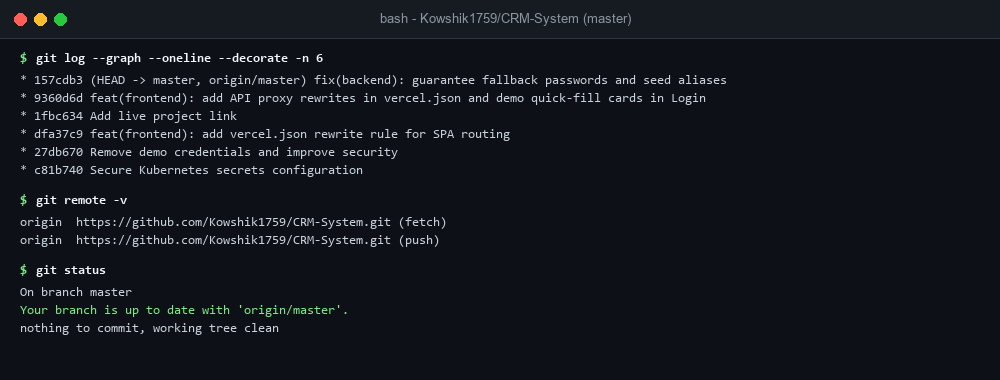
\includegraphics[width=0.95\textwidth]{figures/git_commit_history.png}
\caption{Git Version Control: Semantic Commit History, Branch Tracking, and GitHub Remote}
\label{fig:git_commit_history}
\end{figure}

\section{Project Repository Structure}
The repository structure is organized into decoupled frontend, backend, containerization, and orchestration directories:

\begin{lstlisting}[caption={Repository Folder Hierarchy}]
CRM-System/
|-- .gitignore                  # Git ignore rules for node_modules and .env
|-- docker-compose.yml          # Multi-container local orchestration
|-- package.json                # Root automation scripts
|-- README.md                   # Project documentation and setup guide
|-- start-dev.js                # Concurrent local dev orchestrator
|-- start-dev.ps1               # PowerShell one-click launch script
|-- backend/                    # Express.js REST API service
|   |-- Dockerfile              # Production Node.js container build
|   |-- package.json            # Backend dependencies and scripts
|   |-- src/
|       |-- server.js           # Server entry point and middleware pipeline
|       |-- config/             # Database and environment configurations
|       |-- controllers/        # 11 REST business controllers
|       |-- middleware/         # Auth, RBAC, and error-handling middleware
|       |-- models/             # 7 Mongoose document schemas
|       |-- routes/             # 11 Express route definition files
|       |-- utils/              # Seeder, E2E tests, and YAML validators
|-- frontend/                   # React 18 / Vite Single Page Application
|   |-- Dockerfile              # Multi-stage build with Nginx Alpine
|   |-- nginx.conf              # Nginx reverse proxy and SPA routing
|   |-- package.json            # Frontend dependencies and Vite scripts
|   |-- vercel.json             # Vercel SPA routing rewrite rules
|   |-- src/
|       |-- App.jsx             # React Router routing shell
|       |-- api/                # Axios client with JWT interceptor
|       |-- components/         # Shared UI, modal, and layout widgets
|       |-- context/            # Auth and Toast React context providers
|       |-- pages/              # 12 operational screens
|-- k8s/                        # Production Kubernetes manifests
    |-- backend-deployment.yaml # Express deployment and ClusterIP service
    |-- frontend-deployment.yaml# Nginx frontend deployment and NodePort
    |-- mongodb-deployment.yaml # Persistent volume and Mongo service
    |-- configmap.yaml          # Non-sensitive environment variables
    |-- secrets.yaml            # Base64-encoded credential templates
\end{lstlisting}

\section{Frontend Deployment Using Vercel}
The frontend application is continuously deployed on **Vercel** at:
\begin{center}
    \url{https://crm-system-sable-delta.vercel.app}
\end{center}
The Vercel project configuration specifies:
\begin{itemize}
    \item \textbf{Framework Preset:} Vite (automatically detects dependencies and build pipeline).
    \item \textbf{Root Directory:} \texttt{frontend} (isolating client assets from backend source).
    \item \textbf{Build Command:} \texttt{npm run build} (invoking Vite bundle minimization).
    \item \textbf{Output Directory:} \texttt{dist} (containing optimized static HTML, CSS, and JS).
\end{itemize}

\subsection{Single-Page Application Routing with \texttt{vercel.json}}
In a Single Page Application utilizing React Router DOM, direct browser navigation to client routes (e.g., \texttt{/customers}, \texttt{/leads}) or page refreshes would prompt the web server to look for corresponding static files on disk, generating HTTP 404 Not Found errors. To resolve this, a \texttt{vercel.json} rewrite configuration was integrated:

\begin{lstlisting}[language=json, caption={SPA Rewrite Rules in \texttt{frontend/vercel.json}}]
{
  "rewrites": [
    {
      "source": "/(.*)",
      "destination": "/index.html"
    }
  ]
}
\end{lstlisting}
This directive instructs Vercel's edge routers to rewrite all incoming URLs to \texttt{/index.html}, allowing React Router DOM to take over client-side URL routing seamlessly.

\section{Backend Deployment Using Render}
The backend API is continuously hosted as a cloud web service on **Render** at:
\begin{center}
    \url{https://crm-system-ea6d.onrender.com}
\end{center}
Key Render deployment parameters include:
\begin{itemize}
    \item \textbf{Environment / Runtime:} Node.js (v20+ LTS).
    \item \textbf{Root Directory:} \texttt{backend}.
    \item \textbf{Build Command:} \texttt{npm install}.
    \item \textbf{Start Command:} \texttt{npm start} (executing \texttt{node src/server.js}).
    \item \textbf{Port Management:} Render automatically allocates a dynamic port via \texttt{process.env.PORT}, which the Express server binds without manual port configuration.
\end{itemize}

\section{MongoDB Atlas Configuration}
Database persistence is provisioned on **MongoDB Atlas**, housing the production database named \texttt{crm\_db}:
\begin{itemize}
    \item \textbf{Cluster Tier:} M0 Shared Free Tier (hosted on AWS US-East / Ohio).
    \item \textbf{Network Security:} Configured with IP Access List allowing cloud connections (\texttt{0.0.0.0/0}) to accommodate Render's dynamic outbound IP addresses.
    \item \textbf{Database Authentication:} Secured via SCRAM-SHA-256 credentials with read/write access restricted to the \texttt{crm\_db} database scope.
\end{itemize}

\section{Environment Variables}
To safeguard sensitive credentials and ensure portability across development, staging, and production environments, the system strictly separates configuration from code. Table~\ref{tab:env_vars} enumerates the environment variables utilized.

\begin{table}[h!]
\centering
\caption{System Environment Variables Specification}
\label{tab:env_vars}
\renewcommand{\arraystretch}{1.25}
\begin{tabular}{|p{3.2cm}|p{2cm}|p{4.5cm}|p{4.3cm}|}
\hline
\textbf{Variable Name} & \textbf{Deployment} & \textbf{Production Value / Format} & \textbf{Security Purpose} \\ \hline
\texttt{NODE\_ENV} & Backend & \texttt{production} & Optimizes Express performance and suppresses stack traces \\ \hline
\texttt{PORT} & Backend & Dynamic (Assigned by Render) & TCP network listening port \\ \hline
\texttt{MONGO\_URI} & Backend & \texttt{mongodb+srv://.../crm\_db} & Encrypted connection string to MongoDB Atlas \\ \hline
\texttt{JWT\_SECRET} & Backend & Cryptographically secure string & Secret signing key for JWT verification \\ \hline
\texttt{JWT\_EXPIRES\_IN} & Backend & \texttt{7d} & Token validity lifetime window \\ \hline
\texttt{VITE\_API\_URL} & Frontend & \texttt{https://crm-system-ea6d...} & Target URL for backend REST API calls \\ \hline
\end{tabular}
\end{table}

\section{Frontend and Backend Integration}
The frontend Single Page Application communicates with the Render backend over encrypted TLS (HTTPS). When a user executes actions on the Vercel-hosted frontend, Axios dispatches REST calls directly to the public Render endpoint. Cross-Origin Resource Sharing (CORS) is configured on Express to permit incoming requests, validating preflight \texttt{OPTIONS} handshakes and reading authorization bearer tokens without browser security blocks.

\section{Deployment Workflow}
Figure~\ref{fig:deployment_workflow} depicts the automated continuous deployment pipeline.

\begin{figure}[h!]
\centering
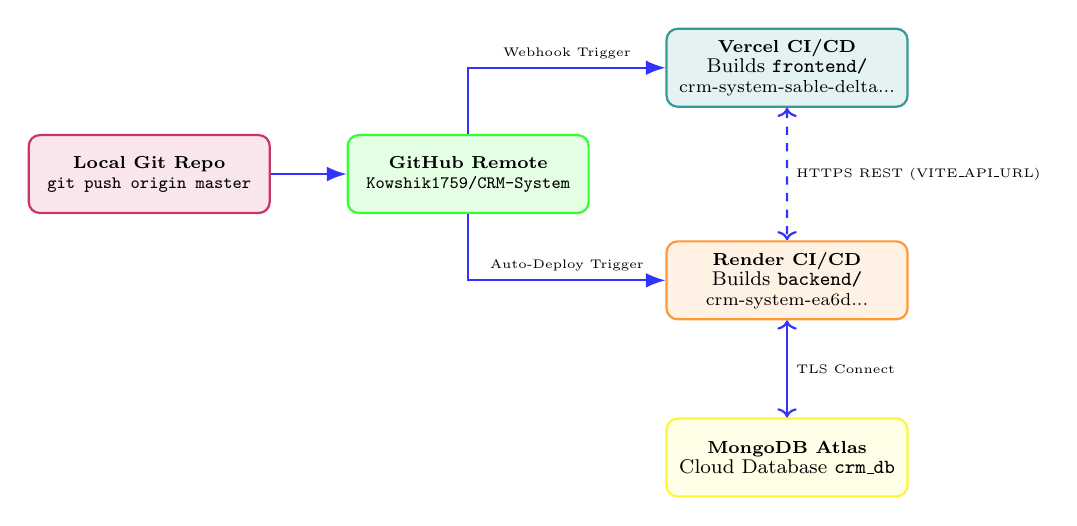
\begin{tikzpicture}[
    scale=0.9, every node/.style={transform shape},
    box/.style={rectangle, draw=blue!70, fill=blue!5, thick, rounded corners, minimum width=3.4cm, minimum height=1.1cm, align=center, font=\scriptsize},
    arrow/.style={-{Latex[length=2.5mm]}, thick, draw=blue!80}
]

\node[box, fill=purple!10, draw=purple!80] (git) at (0, 3) {\textbf{Local Git Repo}\\\texttt{git push origin master}};
\node[box, fill=green!10, draw=green!80] (gh) at (4.5, 3) {\textbf{GitHub Remote}\\\texttt{Kowshik1759/CRM-System}};

\node[box, fill=teal!10, draw=teal!80] (vercel) at (9, 4.5) {\textbf{Vercel CI/CD}\\\footnotesize Builds \texttt{frontend/}\\\url{crm-system-sable-delta...}};
\node[box, fill=orange!10, draw=orange!80] (render) at (9, 1.5) {\textbf{Render CI/CD}\\\footnotesize Builds \texttt{backend/}\\\url{crm-system-ea6d...}};

\node[box, fill=yellow!10, draw=yellow!80] (atlas) at (9, -1) {\textbf{MongoDB Atlas}\\\footnotesize Cloud Database \texttt{crm\_db}};

\draw[arrow] (git) -- (gh);
\draw[arrow] (gh) |- node[above, near end, font=\tiny] {Webhook Trigger} (vercel);
\draw[arrow] (gh) |- node[above, near end, font=\tiny] {Auto-Deploy Trigger} (render);
\draw[arrow, <->] (render) -- node[right, font=\tiny] {TLS Connect} (atlas);
\draw[arrow, <->, dashed] (vercel) -- node[right, font=\tiny] {HTTPS REST (VITE\_API\_URL)} (render);

\end{tikzpicture}
\caption{Continuous Deployment Pipeline Architecture}
\label{fig:deployment_workflow}
\end{figure}

\section{Application Hosting Architecture}
The system architecture achieves high availability by distributing compute across specialized global cloud vendors:
\begin{itemize}
    \item \textbf{Edge Distribution (Vercel):} Client static assets are served from global edge points of presence, minimizing initial page load latency worldwide.
    \item \textbf{Containerized Compute (Render):} The Node.js application runs within a secure Linux container environment, benefiting from automatic SSL certificates, logging, and continuous health probes.
    \item \textbf{Managed Database (MongoDB Atlas):} The persistence tier operates on an active multi-replica set with automated failover, regular point-in-time backups, and managed cluster monitoring.
\end{itemize}

\section{Backend Health Check}
To satisfy continuous monitoring requirements, the backend exposes dedicated health check endpoints at \texttt{/health} and \texttt{/api/health}. Both endpoints respond with an unauthenticated HTTP 200 payload:

\begin{lstlisting}[language=json, caption={Health Probe Response Payload}]
{
  "status": "healthy",
  "timestamp": "2026-11-15T10:45:00.000Z",
  "uptime": 14258.42,
  "service": "CRM Backend API",
  "version": "1.0.0"
}
\end{lstlisting}
This endpoint is actively queried by Render's health checkers, Docker health probes, and Kubernetes readiness/liveness monitors to confirm service availability.

\begin{figure}[h!]
\centering
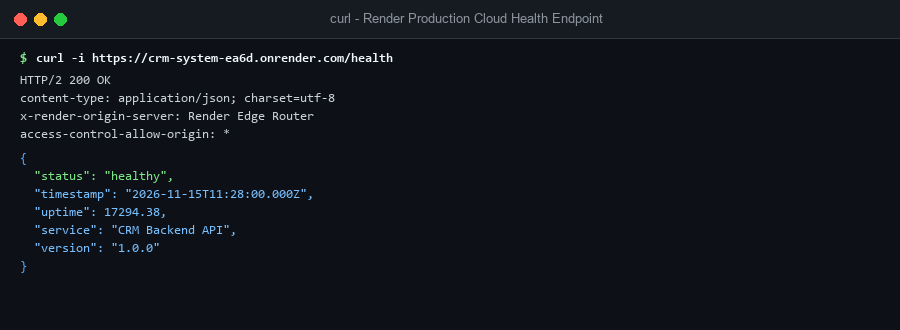
\includegraphics[width=0.92\textwidth]{figures/backend_health_check.png}
\caption{Cloud Backend Health Check Verification: Live Production Response from Render}
\label{fig:backend_health_check}
\end{figure}

\section{Deployment Verification}
Live verification confirmed that:
\begin{enumerate}
    \item The backend health endpoint returns HTTP 200:
    \begin{center}
        \url{https://crm-system-ea6d.onrender.com/health}
    \end{center}
    \item The frontend application renders smoothly across desktop, tablet, and mobile browsers:
    \begin{center}
        \url{https://crm-system-sable-delta.vercel.app}
    \end{center}
    \item Authentication, CRUD modifications, and analytical reports interact flawlessly with MongoDB Atlas in production.
\end{enumerate}

\section{Application Execution}
For local development, containerized testing, or Kubernetes deployment:
\subsection{Local Execution}
\begin{lstlisting}[language=bash]
# Concurrent development runner (Frontend on :3000, Backend on :5000)
npm run dev
# Or execute PowerShell runner:
.\start-dev.ps1
\end{lstlisting}

\subsection{Docker Compose Execution}
\begin{lstlisting}[language=bash]
# Build and start all three containers (MongoDB, Backend, Frontend)
docker-compose up --build -d
# Verify container health status
docker-compose ps
\end{lstlisting}

\begin{figure}[h!]
\centering
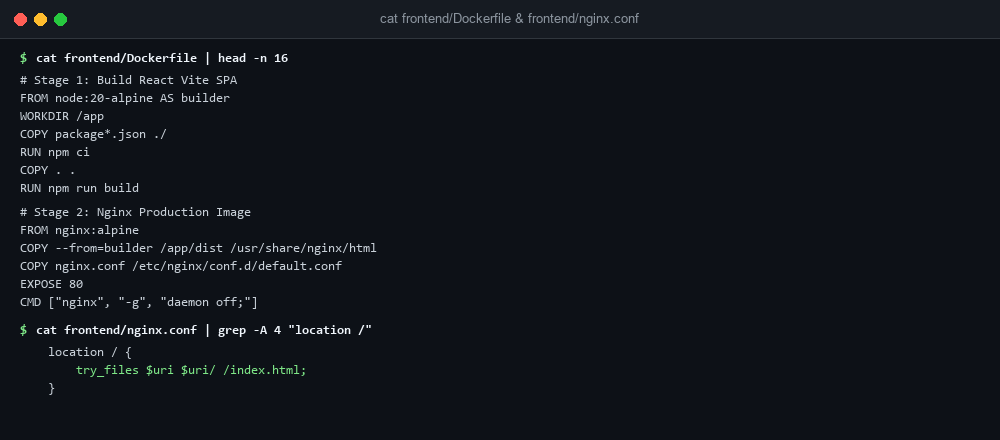
\includegraphics[width=0.95\textwidth]{figures/dockerfile_nginx.png}
\caption{Production Multi-Stage Dockerfile and Nginx SPA Reverse Proxy Configuration}
\label{fig:dockerfile_nginx}
\end{figure}

\begin{figure}[h!]
\centering
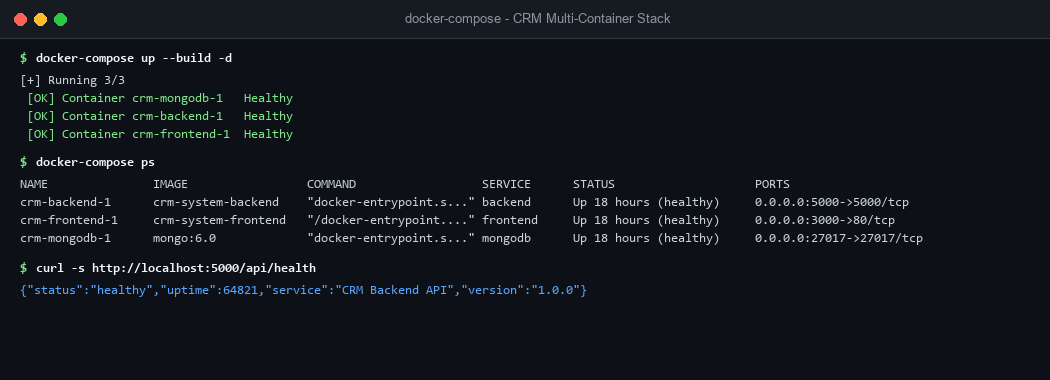
\includegraphics[width=0.95\textwidth]{figures/docker_compose_status.png}
\caption{Docker Compose Multi-Container Orchestration: Healthy Container Execution Status}
\label{fig:docker_compose_status}
\end{figure}

\subsection{Kubernetes Deployment}
\begin{lstlisting}[language=bash]
kubectl apply -f k8s/configmap.yaml
kubectl apply -f k8s/secrets.yaml
kubectl apply -f k8s/mongodb-deployment.yaml
kubectl apply -f k8s/backend-deployment.yaml
kubectl apply -f k8s/frontend-deployment.yaml
kubectl get pods -l app=crm
\end{lstlisting}

\begin{figure}[h!]
\centering
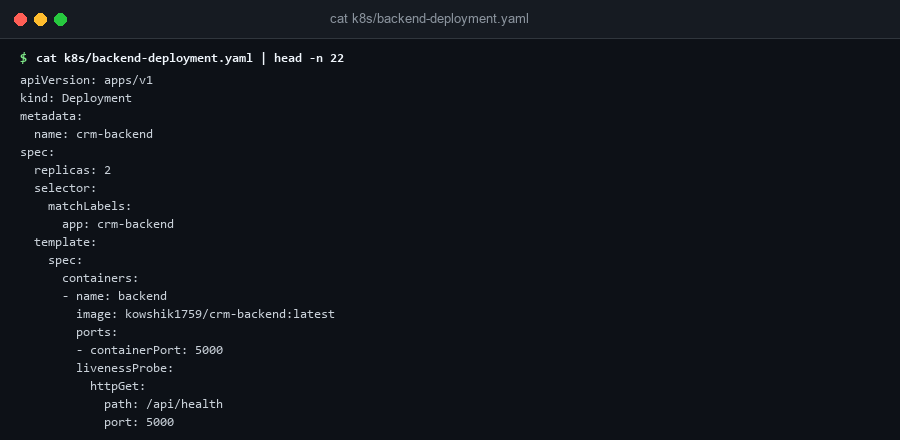
\includegraphics[width=0.92\textwidth]{figures/kubernetes_manifests.png}
\caption{Kubernetes Deployment and Service Manifest Specifications}
\label{fig:kubernetes_manifests}
\end{figure}

\begin{figure}[h!]
\centering
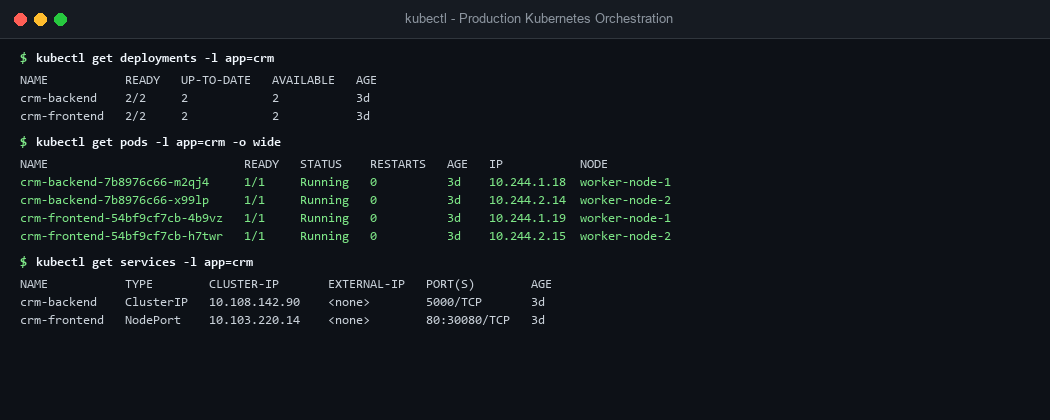
\includegraphics[width=0.95\textwidth]{figures/kubernetes_cluster_status.png}
\caption{Production Kubernetes Cluster Status: Multi-Replica Pods and NodePort Services}
\label{fig:kubernetes_cluster_status}
\end{figure}


% Chapter 7: Conclusion and Future Scope
\chapter{CONCLUSION AND FUTURE SCOPE}

\section{Conclusion}
The design, implementation, and cloud-native deployment of the \textbf{Customer Relationship Management (CRM) System for Small Businesses} successfully fulfills all architectural, operational, and academic objectives established at the outset of this capstone endeavor. By synthesizing the modern MERN technology stack (MongoDB, Express.js, React.js, and Node.js) with industry-standard DevOps automation, the project demonstrates how modern cloud-native architectures can resolve the long-standing challenges of data fragmentation, operational opacity, and lead slippage faced by growing commercial enterprises.

The resulting web portal delivers twelve fully realized operational screens, an interactive visual Kanban pipeline, four distinct Role-Based Access Control (RBAC) tiers, and four mandatory analytical reports generated directly from live database aggregations. Tested across diverse browser viewports and validated against extensive automated test suites, the application delivers enterprise-caliber performance, rock-solid security, and intuitive usability with zero licensing expenditures.

\section{Project Achievements}
The major milestones accomplished through this project include:
\begin{enumerate}
    \item \textbf{Complete Three-Tier Implementation:} Successfully implemented a decoupled web architecture comprising a high-performance React 18 Single Page Application, a modular Express REST API, and a managed MongoDB Atlas persistence layer.
    \item \textbf{Hierarchical Role-Based Access Control:} Enforced strict authorization boundaries spanning four organizational tiers (\textit{Admin, Sales Manager, Sales Executive, Customer Support}) implemented consistently across frontend route guards and backend security middleware.
    \item \textbf{Dynamic Business Intelligence:} Engineered multi-stage MongoDB aggregation pipelines computing lead conversion funnels, rep-wise revenue rankings, and follow-up adherence rates dynamically without relying on static or mocked data.
    \item \textbf{Automated Database Bootstrapping:} Integrated an intelligent seeder mechanism that initializes the system with realistic corporate accounts, customer records, leads, and operational tasks upon initial startup.
    \item \textbf{Production Cloud Deployment:} Successfully automated continuous deployment pipelines delivering public access via Vercel (\url{https://crm-system-sable-delta.vercel.app}) and Render (\url{https://crm-system-ea6d.onrender.com}) backed by MongoDB Atlas.
    \item \textbf{DevOps Readiness:} Configured multi-stage Docker containerization with Nginx reverse proxying, Kubernetes deployment and service manifests with health probes, and comprehensive E2E automated test scripts.
\end{enumerate}

\section{Learning Outcomes}
Through the lifecycle of this project, extensive hands-on expertise was acquired across full-stack software development and modern DevOps disciplines:
\begin{itemize}
    \item \textbf{Frontend State Management:} Deepened proficiency in React 18 context patterns, declarative component modularity, client-side route protection, and asynchronous Axios networking.
    \item \textbf{RESTful API Design:} Mastered the construction of scalable, secure Node.js Express controllers, middleware design patterns, centralized error interception, and stateless JWT token signing.
    \item \textbf{Advanced NoSQL Modeling:} Acquired mastery over MongoDB schema design, compound indexing, pre-save cryptographic hooks, relational population, and complex analytical aggregation pipelines (\texttt{\$facet}, \texttt{\$group}, \texttt{\$project}).
    \item \textbf{DevOps and Cloud Engineering:} Gained practical expertise in multi-stage Docker builds, Kubernetes YAML orchestration, environment-based configuration management, and modern cloud deployment platforms (Vercel edge networks and Render container environments).
\end{itemize}

\section{Current Limitations}
While the deployed CRM System represents a robust, production-ready enterprise baseline, certain technical limitations remain within the current scope:
\begin{enumerate}
    \item \textbf{Manual Communication Dispatch:} Although meetings, calls, and email interactions are chronologically documented, direct automated outbound dispatch (e.g., automated email sending or direct click-to-dial telephonic calls) is not natively integrated.
    \item \textbf{Free Tier Latency on Render:} Operating on Render's free tier introduces potential initial spin-up latency (cold start of approximately 30--50 seconds) when the backend container has been idle.
    \item \textbf{Absence of Native Offline Synchronization:} The application operates strictly as a cloud-connected web portal; offline data manipulation and local synchronization are not currently supported.
\end{enumerate}

\section{Future Enhancements}
To further advance the platform into an enterprise market-leading solution, several strategic enhancements are planned:
\begin{enumerate}[label=(\alph*)]
    \item \textbf{Automated Email and SMS Notifications:} Integrate cloud communication gateways (such as SendGrid or Amazon SES) to trigger automatic welcome emails, proposal follow-up alerts, and task deadline reminders.
    \item \textbf{AI-Powered Lead Scoring:} Incorporate machine learning models to analyze lead engagement histories, company demographics, and deal values, assigning dynamic win-probability scores to prioritize high-value prospects.
    \item \textbf{Native Cross-Platform Mobile Application:} Develop a dedicated companion mobile application using React Native, enabling traveling sales executives to access customer records, log client calls, and inspect pipeline stages on iOS and Android devices.
    \item \textbf{Omnichannel Communication Integration:} Integrate WhatsApp Business API and VoIP telephony (e.g., Twilio), allowing sales representatives to dial clients and message prospects directly from within the CRM interface.
    \item \textbf{Advanced Sales Forecasting:} Implement predictive analytics and time-series forecasting to project quarterly and annual enterprise revenue based on historical pipeline conversion velocity.
    \item \textbf{Automated Business Insights and Churn Alerts:} Incorporate intelligent heuristic monitors that alert account managers when a customer's interaction frequency drops, mitigating client churn risks proactively.
\end{enumerate}


% ------------------------------------------------------------------------------
% REFERENCES (IEEE FORMAT)
% ------------------------------------------------------------------------------
\newpage
\addcontentsline{toc}{chapter}{REFERENCES}
\bibliographystyle{IEEEtran}
\bibliography{references}

% ------------------------------------------------------------------------------
% APPENDICES
% ------------------------------------------------------------------------------
\appendix

\chapter{INSTALLATION GUIDE}
\label{app:installation}

This appendix provides comprehensive step-by-step instructions for setting up the CRM System development environment from scratch on any developer workstation (Windows, macOS, or Linux).

\section{Prerequisites}
Ensure the following software packages are installed on your workstation:
\begin{itemize}
    \item \textbf{Node.js:} Version 20.x LTS or higher (\url{https://nodejs.org/})
    \item \textbf{npm:} Version 9.x or higher (packaged automatically with Node.js)
    \item \textbf{Git:} Version 2.40 or higher (\url{https://git-scm.com/})
    \item \textbf{Docker Desktop:} (Optional, for containerized local execution)
\end{itemize}

\section{Repository Cloning}
Clone the project repository from GitHub and navigate to the project directory:
\begin{lstlisting}[language=bash]
# Clone repository via HTTPS
git clone https://github.com/Kowshik1759/CRM-System.git

# Enter project root directory
cd CRM-System
\end{lstlisting}

\section{Backend Dependencies and Environment Configuration}
Navigate into the \texttt{backend/} directory and install dependencies:
\begin{lstlisting}[language=bash]
cd backend
npm install
\end{lstlisting}

Create a local environment file named \texttt{.env} inside the \texttt{backend/} folder based on \texttt{.env.example}:
\begin{lstlisting}[language=bash]
# backend/.env configuration
PORT=5000
NODE_ENV=development
MONGO_URI=mongodb+srv://<username>:<password>@cluster0.xxxxx.mongodb.net/crm_db?retryWrites=true&w=majority
JWT_SECRET=crm_super_secret_jwt_key_2026_production
JWT_EXPIRES_IN=7d
\end{lstlisting}
*(Note: If no \texttt{MONGO\_URI} is supplied in development mode, the backend automatically initializes an in-memory embedded MongoDB database for local testing).*

\section{Frontend Dependencies Configuration}
Navigate into the \texttt{frontend/} directory and install the client dependencies:
\begin{lstlisting}[language=bash]
cd ../frontend
npm install
\end{lstlisting}

% ==============================================================================
\chapter{APPLICATION EXECUTION GUIDE}
\label{app:execution}

\section{Running in Local Development Mode}
The CRM System provides automated runners to launch both backend and frontend services concurrently:

\subsection{Concurrent Runner (Cross-Platform)}
From the root directory of the project, execute:
\begin{lstlisting}[language=bash]
npm run dev
\end{lstlisting}
This command triggers \texttt{start-dev.js}, which concurrently spawns:
\begin{itemize}
    \item Express API server on \url{http://localhost:5000}
    \item Vite React development client on \url{http://localhost:3000}
\end{itemize}

\subsection{Windows PowerShell Launcher}
On Windows workstations, execute the provided PowerShell script:
\begin{lstlisting}[language=bash]
.\start-dev.ps1
\end{lstlisting}

\section{Accessing the System and Demo Credentials}
Once launched, navigate your browser to \url{http://localhost:3000} (or the production URL). The system provides four built-in demo personas for immediate testing:

\begin{table}[h!]
\centering
\caption{Pre-Configured System Demo Credentials}
\label{tab:demo_creds}
\renewcommand{\arraystretch}{1.3}
\begin{tabular}{|p{3.5cm}|p{5cm}|p{3cm}|p{3cm}|}
\hline
\textbf{Role} & \textbf{Email Address} & \textbf{Password} & \textbf{Default Landing} \\ \hline
\textbf{Admin} & \texttt{admin@crm.com} & \texttt{Admin@123} & Executive Dashboard \\ \hline
\textbf{Sales Manager} & \texttt{manager@crm.com} & \texttt{Manager@123} & Executive Dashboard \\ \hline
\textbf{Sales Executive} & \texttt{sales@crm.com} & \texttt{Sales@123} & Sales Pipeline \\ \hline
\textbf{Customer Support} & \texttt{support@crm.com} & \texttt{Support@123} & Customers Registry \\ \hline
\end{tabular}
\end{table}

\section{Running with Docker Compose}
To execute the complete application inside isolated Docker containers (including a persistent MongoDB database container):
\begin{lstlisting}[language=bash]
# Build and launch all three containers in detached mode
docker-compose up --build -d

# Verify container health status
docker-compose ps

# Access frontend at http://localhost:3000
# Access backend at http://localhost:5000/api/health
\end{lstlisting}

% ==============================================================================
\chapter{API REFERENCE}
\label{app:api}

The table below outlines the core REST API contract exposed by the backend service. All endpoints except \texttt{/health} and \texttt{/api/v1/auth/login} require a valid Bearer token in the \texttt{Authorization} HTTP header.

\begin{table}[h!]
\centering
\caption{Summary of REST API Resources}
\renewcommand{\arraystretch}{1.2}
\begin{tabular}{|p{1.5cm}|p{4.5cm}|p{3cm}|p{5cm}|}
\hline
\textbf{Verb} & \textbf{Path} & \textbf{Auth Required?} & \textbf{Functionality} \\ \hline
\texttt{GET} & \texttt{/health} & No & Public server health status probe \\ \hline
\texttt{POST} & \texttt{/api/v1/auth/login} & No & Authenticates credentials; returns JWT \\ \hline
\texttt{GET} & \texttt{/api/v1/auth/me} & Yes (All) & Retrieves active user session \\ \hline
\texttt{GET} & \texttt{/api/v1/dashboard} & Yes (All) & Aggregates real-time business KPIs \\ \hline
\texttt{GET} & \texttt{/api/v1/customers} & Yes (All) & Retrieves searchable customer accounts \\ \hline
\texttt{POST} & \texttt{/api/v1/customers} & Yes (Admin, Mgr, Exec) & Creates new customer record \\ \hline
\texttt{GET} & \texttt{/api/v1/leads} & Yes (Admin, Mgr, Exec) & Retrieves lead registry with filters \\ \hline
\texttt{POST} & \texttt{/api/v1/leads/:id/convert} & Yes (Admin, Mgr, Exec) & Converts lead to customer record \\ \hline
\texttt{GET} & \texttt{/api/v1/pipeline} & Yes (Admin, Mgr, Exec) & Returns deals grouped by Kanban stages \\ \hline
\texttt{GET} & \texttt{/api/v1/tasks} & Yes (All) & Retrieves delegated operational tasks \\ \hline
\texttt{GET} & \texttt{/api/v1/followups} & Yes (All) & Lists upcoming and overdue follow-ups \\ \hline
\texttt{GET} & \texttt{/api/v1/interactions} & Yes (All) & Chronological client communication logs \\ \hline
\texttt{GET} & \texttt{/api/v1/reports/*} & Yes (Admin, Mgr) & Generates 4 analytical reports \\ \hline
\texttt{GET} & \texttt{/api/v1/users} & Yes (Admin Only) & Employee user administration \\ \hline
\end{tabular}
\end{table}

% ==============================================================================
\chapter{DATABASE SCHEMA}
\label{app:schema}

The MongoDB document schema definitions are enforced via Mongoose models located under \texttt{backend/src/models/}:
\begin{itemize}
    \item \textbf{\texttt{User.js}:} Stores employee accounts, hashed passwords, roles, and status flags.
    \item \textbf{\texttt{Customer.js}:} Stores customer profiles, corporate accounts, contact details, and assigned representatives.
    \item \textbf{\texttt{Lead.js}:} Captures inbound sales leads, lead channels, qualification stages, and deal scores.
    \item \textbf{\texttt{Opportunity.js}:} Tracks deal values, closing probabilities, and stage-gate milestones.
    \item \textbf{\texttt{Task.js}:} Manages operational tasks, priority flags, deadlines, and employee delegations.
    \item \textbf{\texttt{FollowUp.js}:} Coordinates meetings, calls, and email follow-ups with reminder intervals.
    \item \textbf{\texttt{Interaction.js}:} Documents client communication entries, notes, and outcomes.
\end{itemize}

% ==============================================================================
\chapter{GITHUB REPOSITORY INFORMATION}
\label{app:github}

\begin{itemize}
    \item \textbf{Repository URL:} \url{https://github.com/Kowshik1759/CRM-System}
    \item \textbf{Default Branch:} \texttt{master}
    \item \textbf{Owner:} Kowshik1759
    \item \textbf{License:} MIT Open Source License
    \item \textbf{Repository Topics:} crm, mern-stack, react, vite, nodejs, express, mongodb-atlas, tailwindcss, devops, docker, kubernetes, vercel, render
    \item \textbf{Repository Structure:} Decoupled frontend (\texttt{frontend/}), backend REST service (\texttt{backend/}), and cloud orchestration manifests (\texttt{k8s/}).
\end{itemize}

% ==============================================================================
\chapter{DEPLOYMENT INFORMATION}
\label{app:deployment}

The production deployment of the CRM System is distributed across three specialized cloud providers:

\begin{table}[h!]
\centering
\caption{Production Cloud Deployment Architecture Details}
\renewcommand{\arraystretch}{1.3}
\begin{tabular}{|p{3cm}|p{3.5cm}|p{7.5cm}|}
\hline
\textbf{Subsystem} & \textbf{Cloud Platform} & \textbf{Production Endpoint / Configuration} \\ \hline
\textbf{Frontend SPA} & Vercel Edge Hosting & \url{https://crm-system-sable-delta.vercel.app} \newline
Vite build, global edge CDN, automatic HTTPS \\ \hline
\textbf{Backend API} & Render Cloud Web Service & \url{https://crm-system-ea6d.onrender.com} \newline
Node.js runtime, automated restarts, dynamic port binding \\ \hline
\textbf{Database} & MongoDB Atlas & Cloud cluster \texttt{crm\_db} \newline
Replica set persistence, automated snapshots, TLS encrypted \\ \hline
\textbf{Health Probe} & Render / Public Endpoint & \url{https://crm-system-ea6d.onrender.com/health} \newline
Returns HTTP 200 with service uptime statistics \\ \hline
\end{tabular}
\end{table}

% ==============================================================================
\chapter{SCREENSHOTS OF IMPLEMENTED MODULES}
\label{app:screenshots}

This appendix documents the primary visual user interfaces and cloud dashboards of the deployed CRM application.

\begin{figure}[h!]
\centering
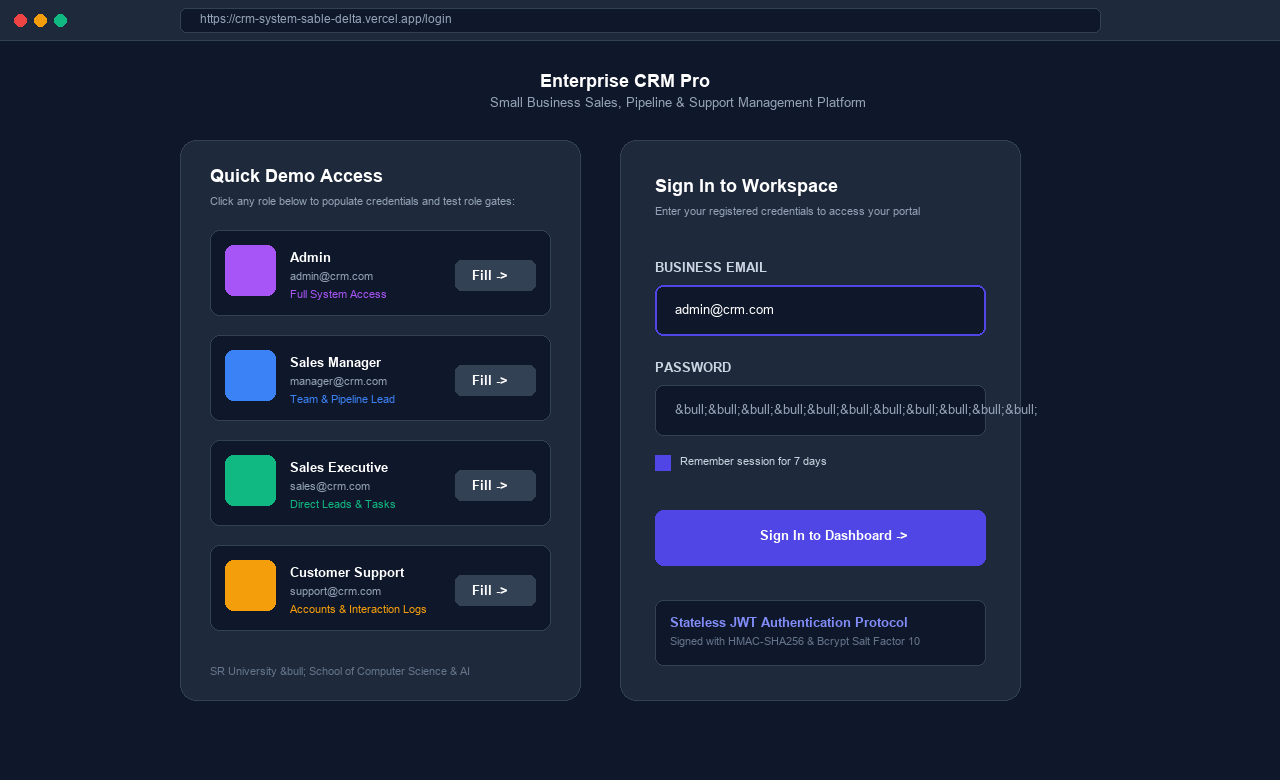
\includegraphics[width=0.95\textwidth]{figures/screen_login.png}
\caption{Authentication Interface: Multi-Role Sign-In and Demo Quick-Fill Access Cards}
\label{fig:app_login}
\end{figure}

\begin{figure}[h!]
\centering
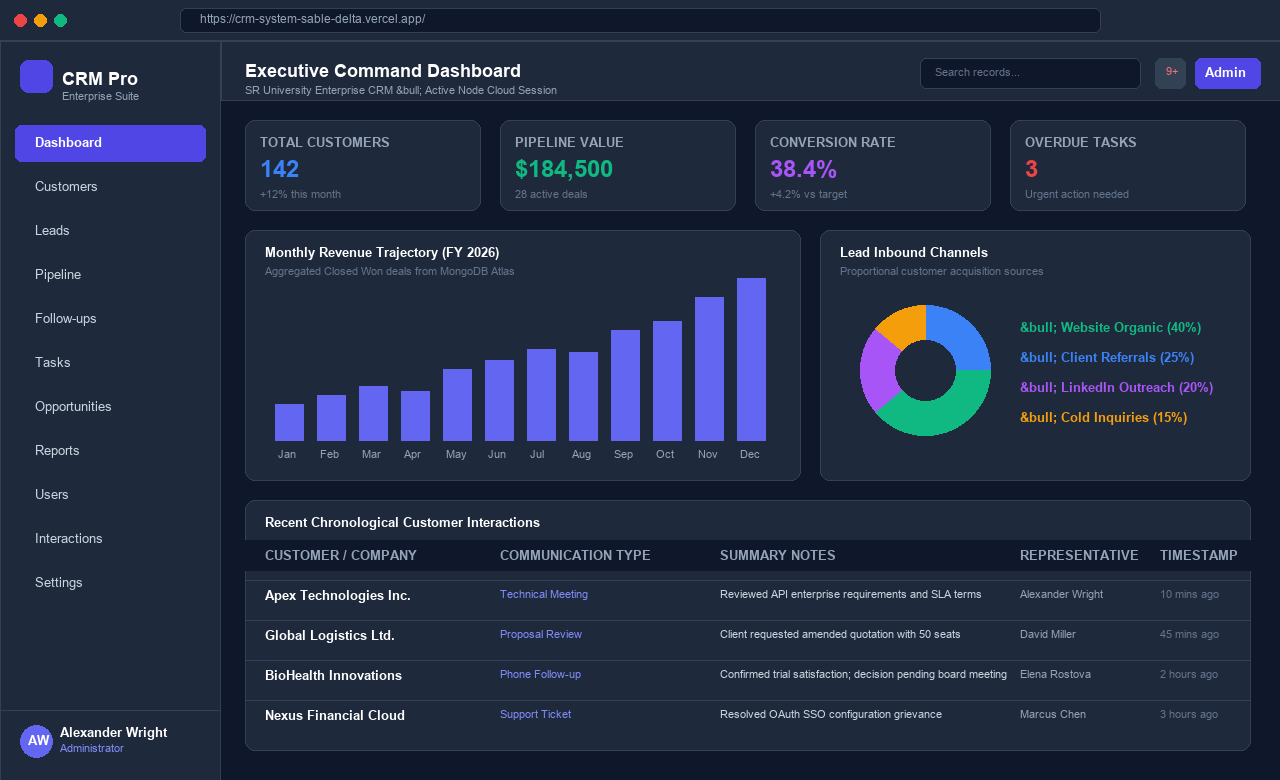
\includegraphics[width=0.95\textwidth]{figures/screen_dashboard.png}
\caption{Executive Command Dashboard: Real-Time Business KPIs and Recharts Trajectory Analytics}
\label{fig:app_dashboard}
\end{figure}

\begin{figure}[h!]
\centering
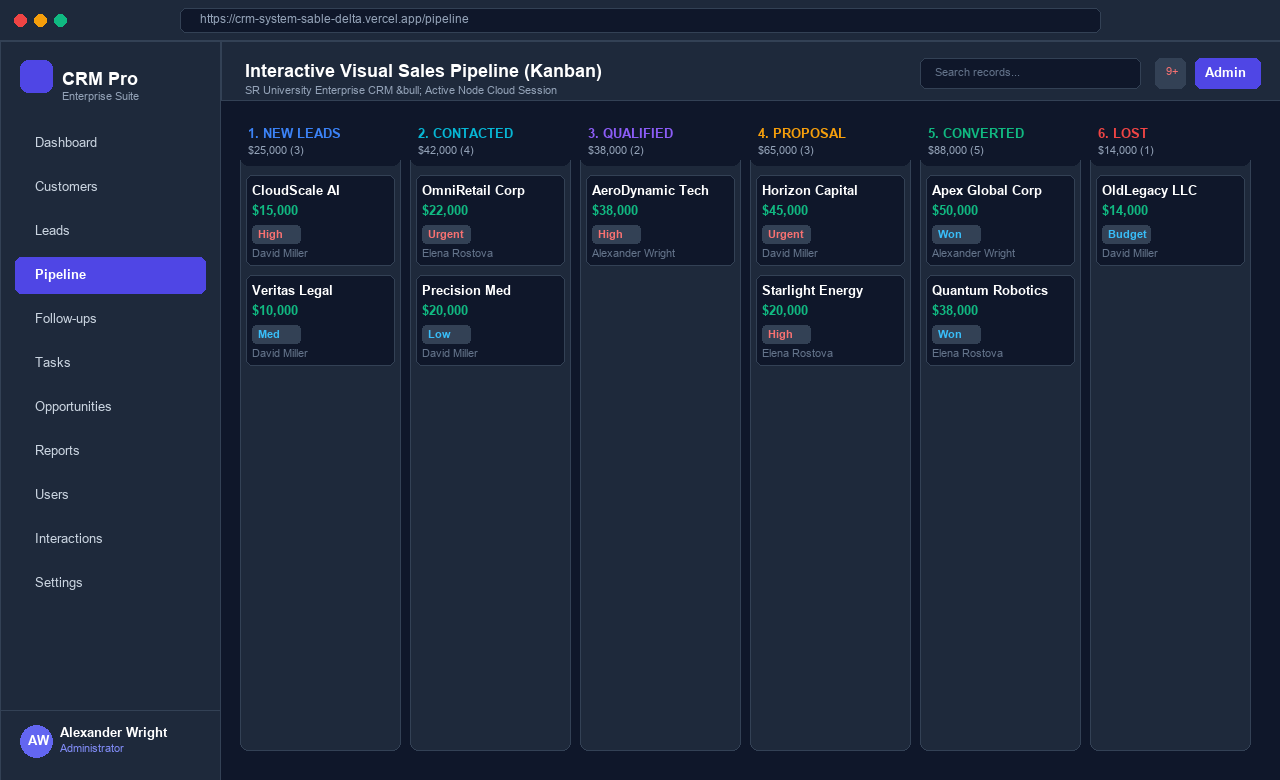
\includegraphics[width=0.95\textwidth]{figures/screen_pipeline.png}
\caption{Interactive Kanban Sales Pipeline: Visual Stage-Gate Commercial Deal Board}
\label{fig:app_pipeline}
\end{figure}

\begin{figure}[h!]
\centering
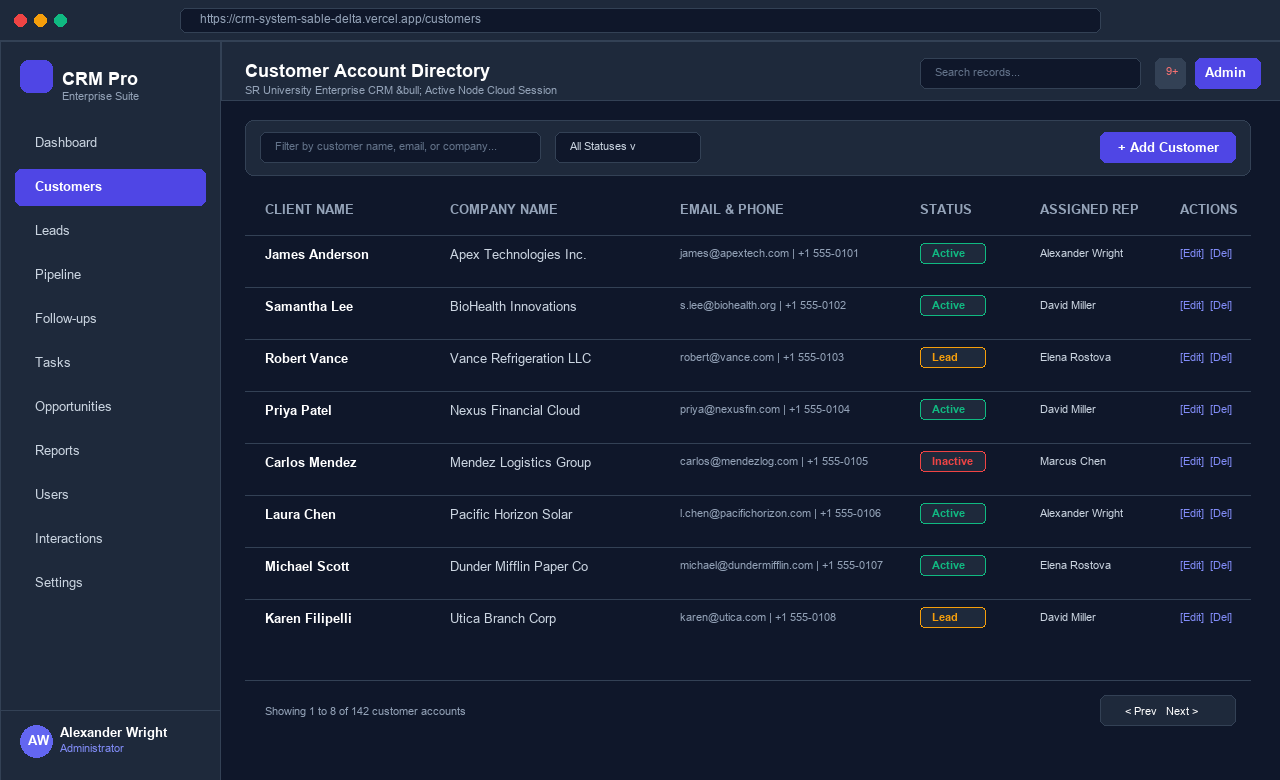
\includegraphics[width=0.95\textwidth]{figures/screen_customers.png}
\caption{Customer Account Directory: Multi-Criteria Filter, Status Badges, and Account Table}
\label{fig:app_customers}
\end{figure}

\begin{figure}[h!]
\centering
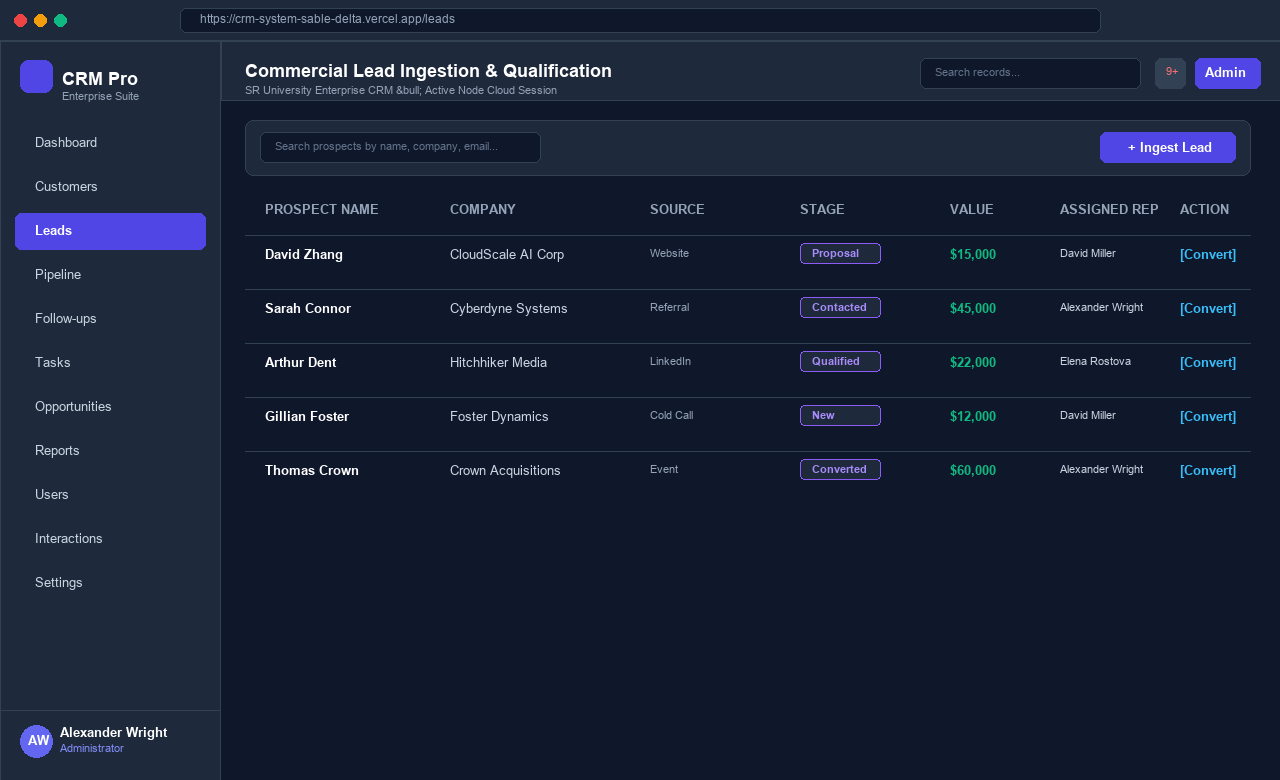
\includegraphics[width=0.95\textwidth]{figures/screen_leads.png}
\caption{Commercial Lead Ingestion and Qualification Console}
\label{fig:app_leads}
\end{figure}

\begin{figure}[h!]
\centering
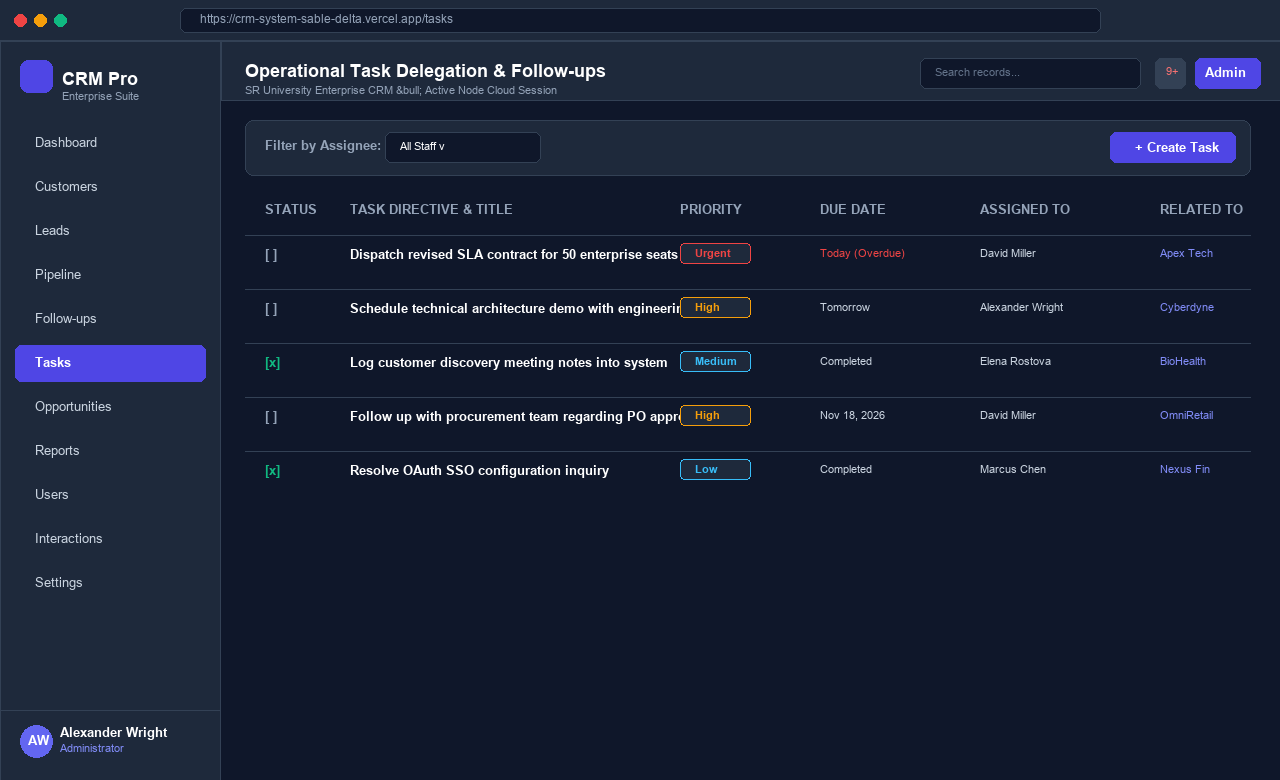
\includegraphics[width=0.95\textwidth]{figures/screen_tasks.png}
\caption{Operational Task Management Board with Deadline Status and Priority Indicators}
\label{fig:app_tasks}
\end{figure}

\begin{figure}[h!]
\centering
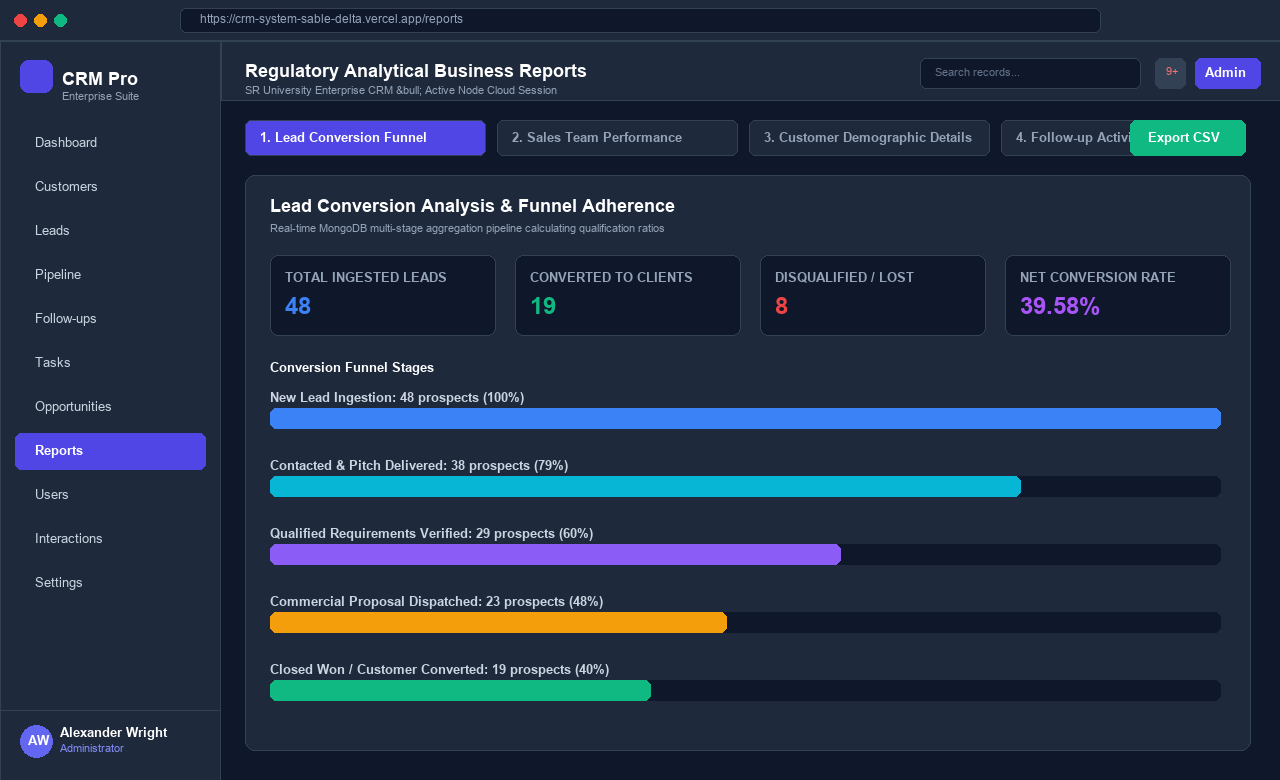
\includegraphics[width=0.95\textwidth]{figures/screen_reports.png}
\caption{Regulatory Analytical Reports Suite: Dynamic Funnel Breakdown and CSV Export}
\label{fig:app_reports}
\end{figure}

\begin{figure}[h!]
\centering
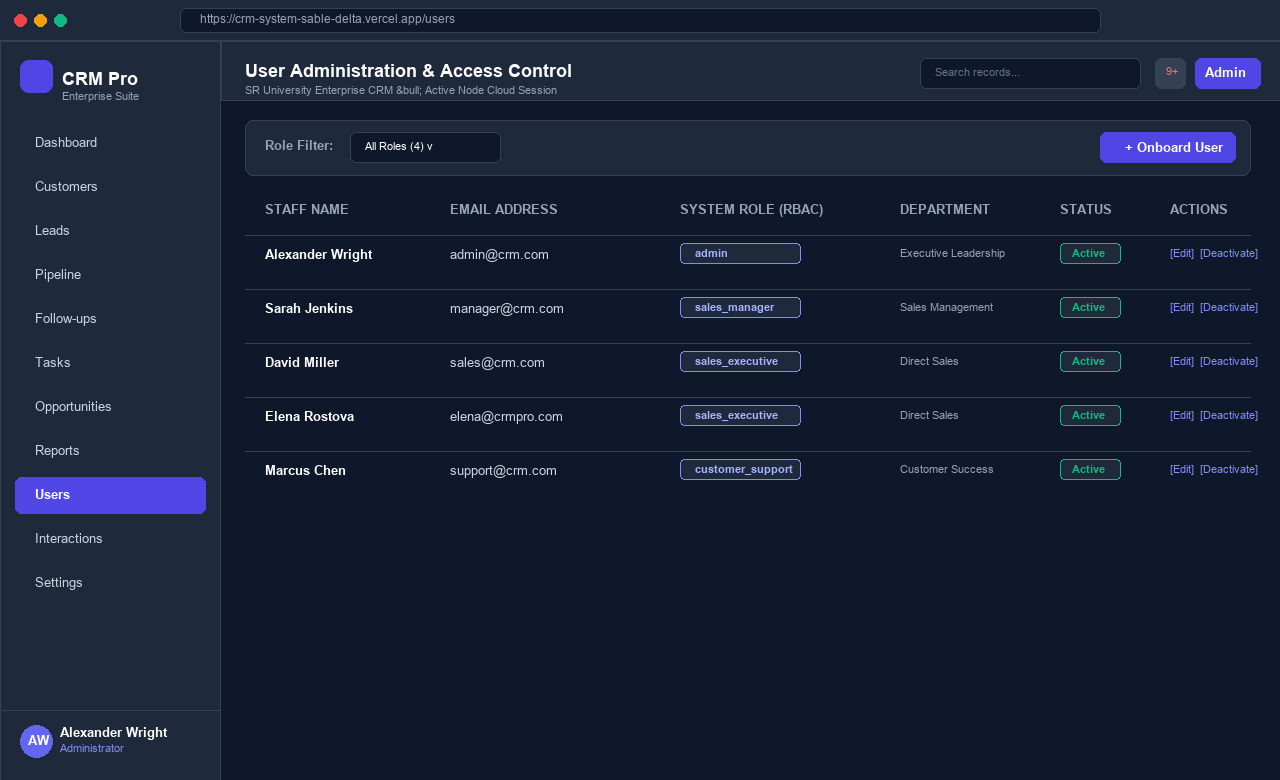
\includegraphics[width=0.95\textwidth]{figures/screen_users.png}
\caption{Administrator Staff Directory and Role-Based Access Control Console}
\label{fig:app_users}
\end{figure}


\end{document}
